\chapter{Scientific Dissemination}

During this thesis, I have produced~{\color[rgb]{0.9,0.2,0.16}\footnote{For an up-to-date list of my contributions, see my \emph{ResearchGate} profile: \href{https://www.researchgate.net/profile/Pamphile\_Roy}{https://www.researchgate.net/profile/Pamphile\_Roy}}}:

\begin{enumerate}
\item[\textbf{7}] accepted and published articles,
\item[\textbf{6}] communications in conferences,
\item[\textbf{3}] reviews in international journals.
\end{enumerate}

\addcontentsline{toc}{section}{Articles}
\nociteJbib*
\bibliographystyleJbib{unsrt}
\bibliographyJbib{my_biblio_article}

\addcontentsline{toc}{section}{Conferences}
\nociteCbib*
\bibliographystyleCbib{unsrt}
\bibliographyCbib{my_biblio_communication}

\addcontentsline{toc}{section}{Reviews}
\section*{Reviews}

I have been reviewing manuscripts in the following journals~{\color[rgb]{0.9,0.2,0.16}\footnote{Reviews have been verified on \emph{publons}: \href{https://publons.com/a/1567681}{publons.com/a/1567681}}}:

\begin{itemize}
\item Computational Geosciences,
\item Stochastic Environmental Research and Risk Assessment,
\item Computer Methods in Applied Mechanics and Engineering.
\end{itemize}

\chapter{Batman}

\section{Description}
Bayesian Analysis Tool for Modelling and uncertAinty quaNtification (batman) is an open source Python package dedicated to statistical analysis based on non-intrusive ensemble experiment.

\emph{batman} library provides a convenient, modular and efficient framework for design of experiments, surrogate model and uncertainty quantification. *batman* relies on open source python packages dedicated to statistics (*openTURNS* and *scikit-learn* [@openturns, @scikit-learn]). It also implements advanced methods for resampling, robust optimization and uncertainty visualization [@roy2017a].

*batman* handles the workflow for statistical analysis. It makes the most of HPC resources by managing asynchronous parallel tasks. The internal parallelism of each task does not conflict with *batman*'s parallel environment.

*batman* analysis is launched from a *command line interface* and a setting file. *batman* functionalities can also be accessed through an API.

*batman* is CECILL-B licensed; it is actively developed and maintained by researchers at CERFACS.

\section{Implementation}



\section{Dissemination}


\chapter{Constructing a Design of Experiments}\label{chap:doe}

This work proposes a new stochastic, iterative DoE ---\thinspace named KDOE\thinspace--- based on a modified Kernel Density Estimation (KDE). It is a two-step process: \emph{(i)} candidate samples are generated using MCMC based on KDE, and \emph{(ii)} one of them is selected based on some metric. The performance of the method is assessed by means of the $C^2$-discrepancy space-filling criterion. KDOE appears to be as performant as classical one-shot methods in low dimensions, while it presents increased performance for high-dimensional parameter spaces. This work proposes a new  methodology to stochastically sample the input parameter space iteratively allowing, at the same time, to take into account any constrains, such as non-rectangular DoE~\citep{Lekivetz2015}, sensitivity indices or even constrains on the quality on particular subprojections as in~\citep{Joseph2015}. It is a versatile method which offers an alternative to classical methods and, at the same time, is easy to implement and offers customization based on the objective of the DoE.

\section{Presentation of the method}\label{sec:method}

In its basis form, our adaptive sampling strategy consists in adding a point far from the existing points in the parameter space. The notion of distance corresponds to a measure of discrepancy. However, instead of considering the whole hypercube, the technique proposed only focuses on empty regions defined using an Exclusion Field (EF). This exclusion field describes the probability of selecting a new point depending on its position.

By means of utilizing EF, it becomes possible to generate new samples that are located preferentially in these empty regions. Then, out of the $n_{gen}$ generated samples from the EF, the one that leads to the best value of some criterion is selected. It is to be noted that there is no optimization process in the sense that it is just a selection process based on probable samples of the EF. The whole process ensures randomness in the generation of the parameter space. Its algorithm is shown in~\cref{alg:doe}. %Hereafter, this method is referred to as the KDOE method.

\Cref{sec:kde} introduces the EF, and \cref{sec:sample} describes the sampling procedure from the EF. Agorithm \ref{alg:doe} gives an overview of the method. In the following, it is referred to as the Kernel-DoE (KDOE) method. 

\begin{algorithm}
  \caption{Sampling Strategy: Kernel-DoE}
  \label{alg:doe}
  \begin{algorithmic}[1]
  \Require $\mathbf{X}^{N_s}_d$, $N_{max}$, $N_s$, $n_{gen}$
  \Comment{Start from a sample $\mathbf{X}^{N_s}_d$ composed of $N_s$ samples in dimension $d$}
  \While{$N_s < N_{max}$}
    \State $f \gets$ Construction of the Exclusions Field from $\mathbf{X}^{N_s}_d$
    \State $\mathbf{Y}^{n_{gen}}_d \gets$ pick $n_{gen}$ samples using Metropolis-Hasting MCMC
    \State $\mathbf{Y}^{j}_d \gets$ point in $N_{gen}$ which minimize the discrepancy
	\State $\mathbf{X}^{N_s + 1}_d \gets \left\{\mathbf{X}^{N_s}_d, \mathbf{Y}^{j}_d \right\}$
  \EndWhile
  \end{algorithmic}
\end{algorithm}




\subsection{Determination of the exclusion field}\label{sec:kde}

It is assumed that there are $N_s$ samples that have already been selected. The spatial probability density function used to draw a new sample is given by:
\begin{align}
f(\mathbf{x}) &= 1 - \sum_{i=1}^{N_{s}} K\left(\mathbf{x},\mathbf{x}^{(i)}\right) \, .
\end{align}
It is reminded that the $N_s$ samples that have already been chosen are noted $\mathbf{x}^{(i)}$, with $i$ between 1 and $N_s$. The dimension is noted $d$ and $K$ is a Gaussian kernel---expressed as in~\cref{eq:kde}.

The general idea is to reduce the probability of selecting a new point close to the samples already drawn. Hence a zone of exclusion is created around each of the already selected points, with a width parametrized by $h$. The parameter $h$ has been set to $h = \frac{\sigma}{N_s^{1/d}}$ with $\sigma=0.3$. This allows us to have a width of exclusion that decreases as the number of samples increases.

Moreover, the probability is set to 0 outside of the unit hypercube in order to prevent sampling outside of the region of interest. Note that this probability is not normalized. This is not a problem because the sampling procedure does not requires this property, as it will be shown in the next section.

The expression of the distance function $D$ is used to generate many different shapes. In our case, alignment of samples on each axis should be avoided as done with Latin Hypercube Sampling designs. This is achieved by using a Minkowski distance~\citep{Cha2007} for $D$:
\begin{align}
D\left(\mathbf{x},\mathbf{x}^{(i)}\right)=\left(\sum_{j=1}^d |x_{j}-x_{ij}|^p\right)^{1/p},
\end{align}
where $p$ is the order of the distance. Setting $p < 1$ leads to a \emph{star shape}, as shown in~\cref{fig:minkowsky} where one sample has already been selected. In the following, $p=0.5$ is used. In~\cref{fig:3d_kde}, three samples have already been selected. The star shape is present in all dimensions. Moreover, these shapes interact with each other as they cross as shown in \cref{fig:inter_kde}. In this case $\sigma=0.8$ to highlight this property.

\begin{figure}[!h]               
\centering
%\subfloat[Wrap-around discrepancy]{
%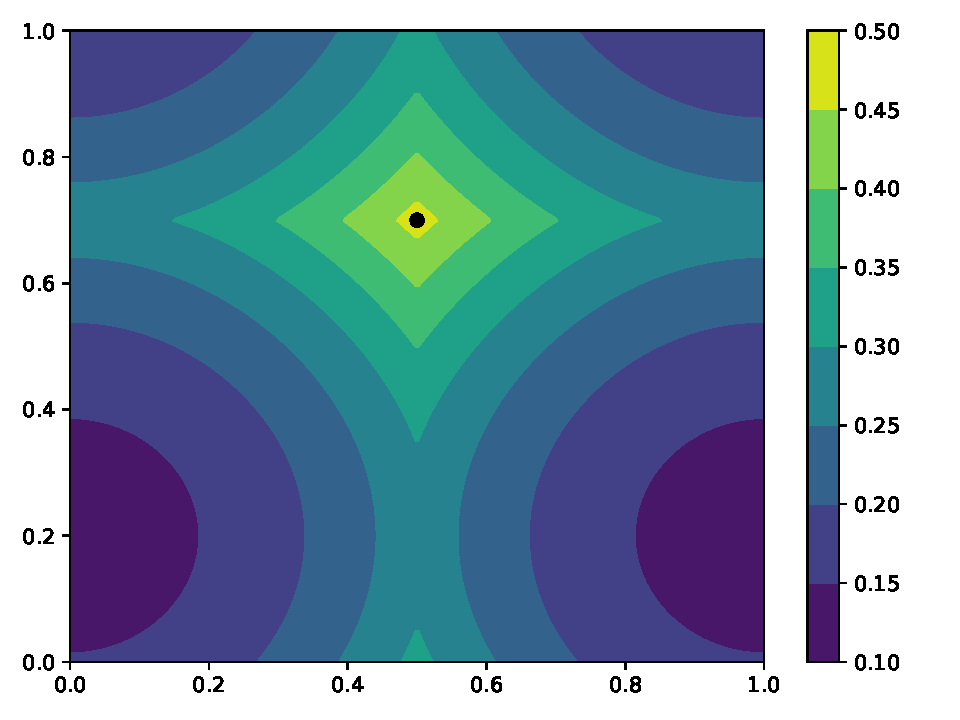
\includegraphics[width=0.49\linewidth,height=\textheight,keepaspectratio]{fig/contributions/doe/wrap_disc.pdf}}
%~
%\subfloat[Inverse Mindkowsky distance]{
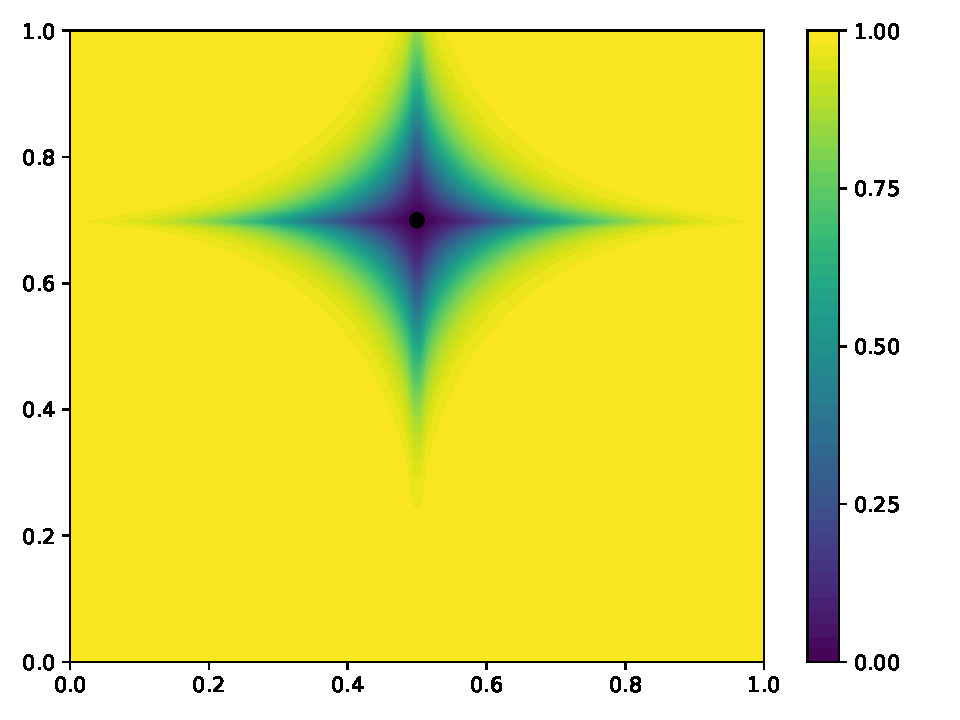
\includegraphics[width=0.8\linewidth,height=\textheight,keepaspectratio]{fig/contributions/doe/inv_minkowsky.pdf}
%}
\caption{Probability density in a 2-dimensional parameter space. \emph{Dot} represents the sample already drawn at (0.5, 0.7).}
 \label{fig:minkowsky}
\end{figure}

\begin{figure}[!h]
\centering
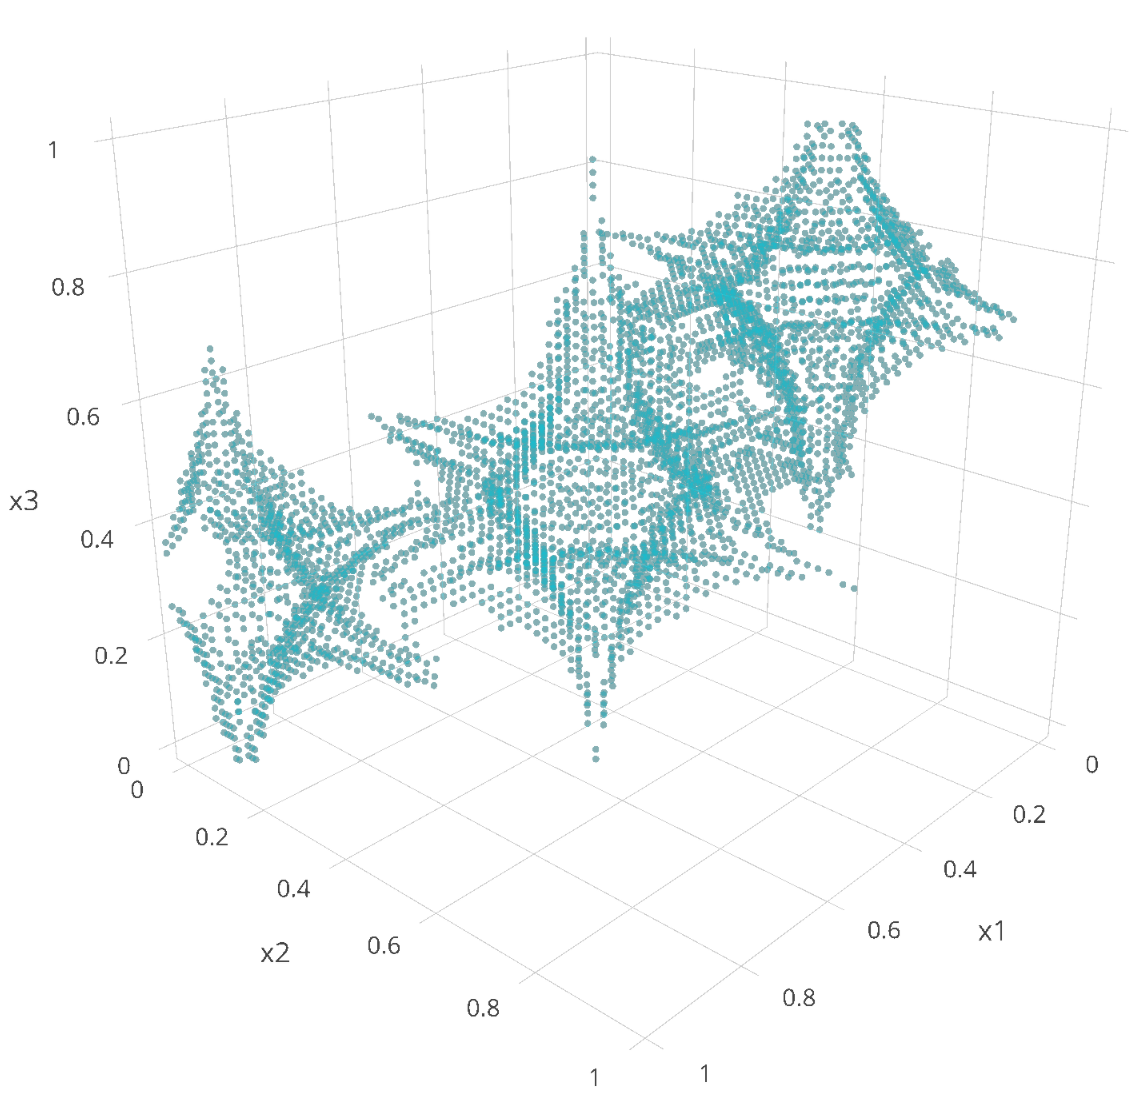
\includegraphics[width=0.8\linewidth,keepaspectratio]{fig/contributions/doe/3d_star.png}
\caption{Scatter plot representation of a 3-dimensional KDE with three points in the parameter space. Points represents an iso contour of probability.}
\label{fig:3d_kde}
\end{figure}

\cleardoublepage

\begin{figure}[!h]
\centering
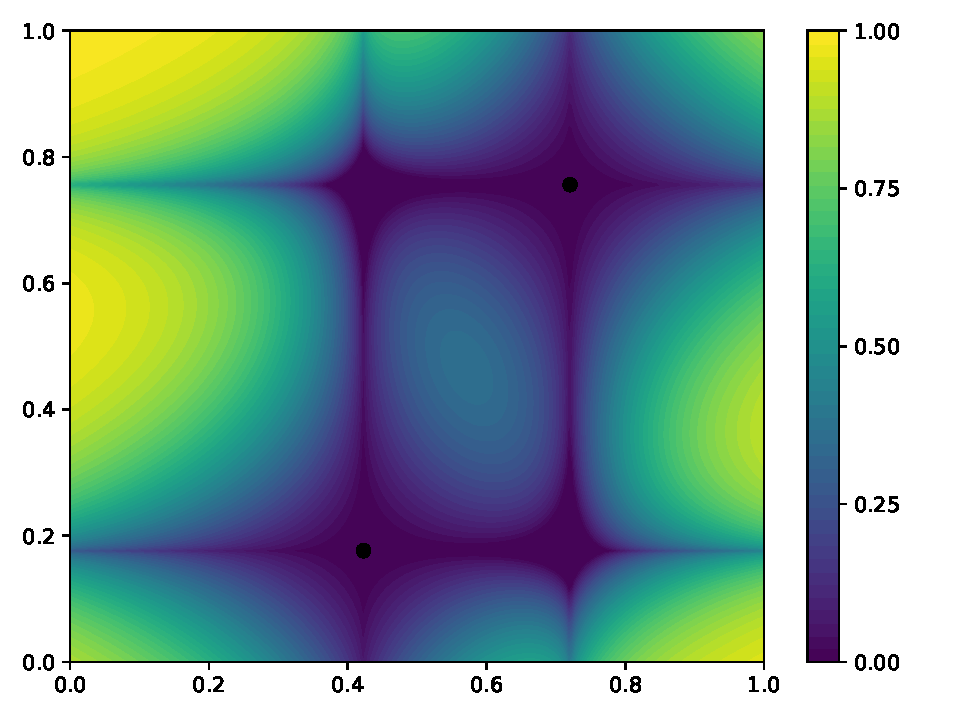
\includegraphics[width=0.8\linewidth,keepaspectratio]{fig/contributions/doe/kde_inter.pdf}
\caption{Interaction effects on the probability density in a 2-dimensional parameter space. \emph{Dots} represent 2 existing samples.}
\label{fig:inter_kde}
\end{figure}


\subsection{Sampling and selection procedures}\label{sec:sample}

%Using the modified version of the KDE, it is possible to generate samples following the posterior distribution.

The classical way to sample from a PDF is to use the inverse transform sampling method. However, finding the inverse cumulative distribution function of a complex PDF can be computationally intensive ---\thinspace the cost increases with dimensionality. The \emph{Metropolis-Hasting}~\citep{Hastings1979} algorithm was selected as an efficient way to sample from $f$. Contrary to methods such as HMC or NUTS~\citep{Hoffman2011}, it does not require the calculation of the gradient of the log-probability density function, which is a costly operation. This algorithm provides a random walk of the parameter space that converges toward the target PDF.

%Using an arbitrary distribution $g(\mathbf{x}|\mathbf{y})$, a new candidate $\mathbf{x}$ is evaluated based on the previous point $\mathbf{y}$. This property makes it a \emph{Markov Chain} as the current value is only conditioned by the previous one. The distribution $g$ is chosen as a Gaussian PDF so that samples close to the previous one are preferably sampled. This algorithm provides a random walk of the parameter space that converges toward the target PDF.


\Cref{fig:sample_kde} shows an example with two initial points already selected in the hypercube $[0, 1]^2$. Based on these two points (\emph{dots}), $f$ is build and new samples are drawn (\emph{squares}).

\begin{figure}[!h]
\centering
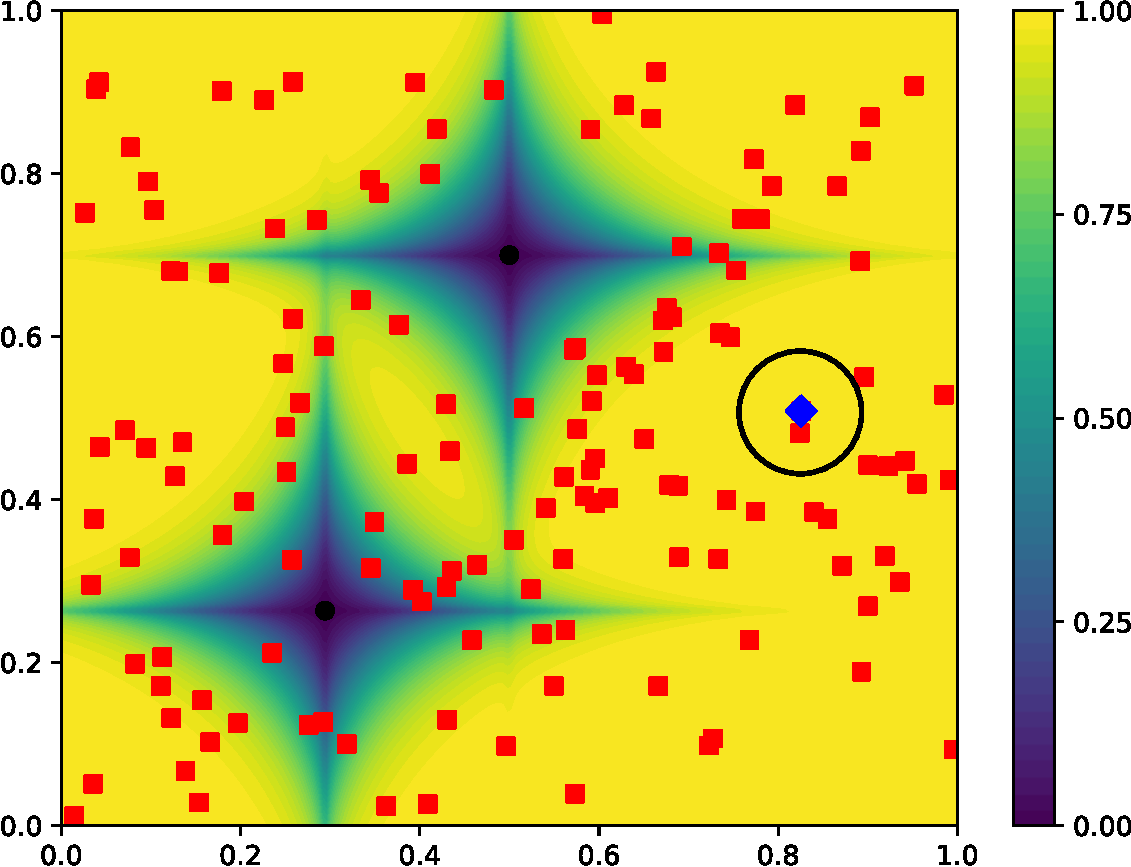
\includegraphics[width=0.7\linewidth,keepaspectratio]{fig/contributions/doe/sampling_KDE.pdf}
\caption{Probability density in a 2-dimensional parameter space. \emph{Dots} represent the samples already drawn, \emph{squares} are the result of the Metropolis-Hasting sampling and \emph{circled-diamond} is the sample selected based on the resulting centred discrepancy.}
\label{fig:sample_kde}
\end{figure}

The next step consists in choosing a new sample from these candidates. Any metric can be chosen here depending on the final objective. In the following, we focused on the uniformity of the DoE. Hence, the centred discrepancy $C^2$ is used~\citep{Fang2006}---see~\cref{eq:c2}. Since the lowest values of $C^2$-discrepancy result in more uniform samples, the sample minimizing it is chosen (\emph{circled-diamond}). Thus, this iterative procedure acts like and optimizer on the $C^2$-discrepancy where the candidates are not drawn totally randomly but with the knowledge of the current samples. \Cref{fig:star} shows an example with 10 points. The initial sample consisted of one point. The result is a low discrepancy sample constructed iteratively.

\begin{figure}[!h]
\centering
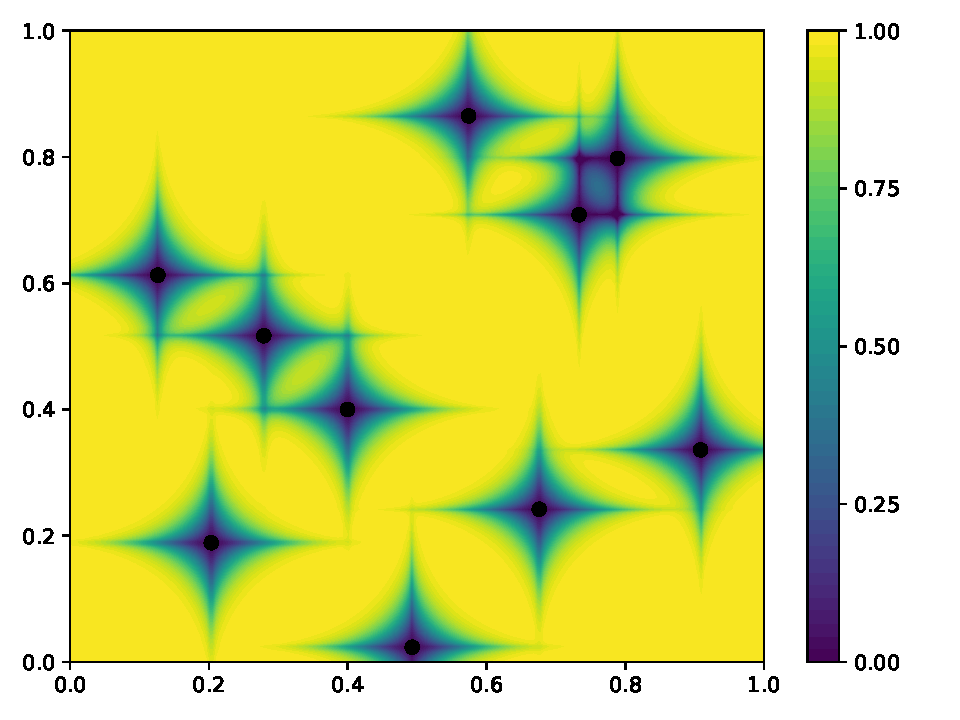
\includegraphics[width=0.9\linewidth,keepaspectratio]{fig/contributions/doe/10_star.pdf}
\caption{Probability density in a 2-dimensional parameter space. The 10 \emph{dots} represent the samples used to fit the KDE.}
\label{fig:star}
\end{figure}

The method is not deterministic which is useful if one wants to generate a new independent set of experiments. To compute sensitivity indices of \emph{Sobol'}, two independent samples are required~\citep{Saltelli2010}. As stated in~\citep{Saltelli2010}, quasi-random sequences such as \emph{Sobol'} are classically used but, as they are deterministic, it is not possible to generate an independent sample directly. One possibility is to get these two samples as one sample of shape $X_{2d}^{N_s}$. Splitting the matrix column wise-like ensures independence of the samples. However, as the dimensionality increases, the quality of the sequence deteriorates ($d > 10$). Hence, this technique is limited to a small number of dimensions. Our method does not share this limitation.

As stated, $n_{gen}$ candidate samples are generated through MCMC. \Cref{fig:conv-ngen} presents a convergence analysis of the quality of the final design $X_2^{40}$ depending on the size of the MCMC sample at each iteration. Confidence intervals are calculated using 100 realizations of the same parametrization. The discrepancy converges to its final value after $n_{gen}>100$. This allows to control the computational cost required to generate the DoE. Various configurations of $X_d^{N_s}$ have been tested and results are similar. In the following, $n_{gen}$ was fixed to 100.

\begin{figure}[!h]
\centering
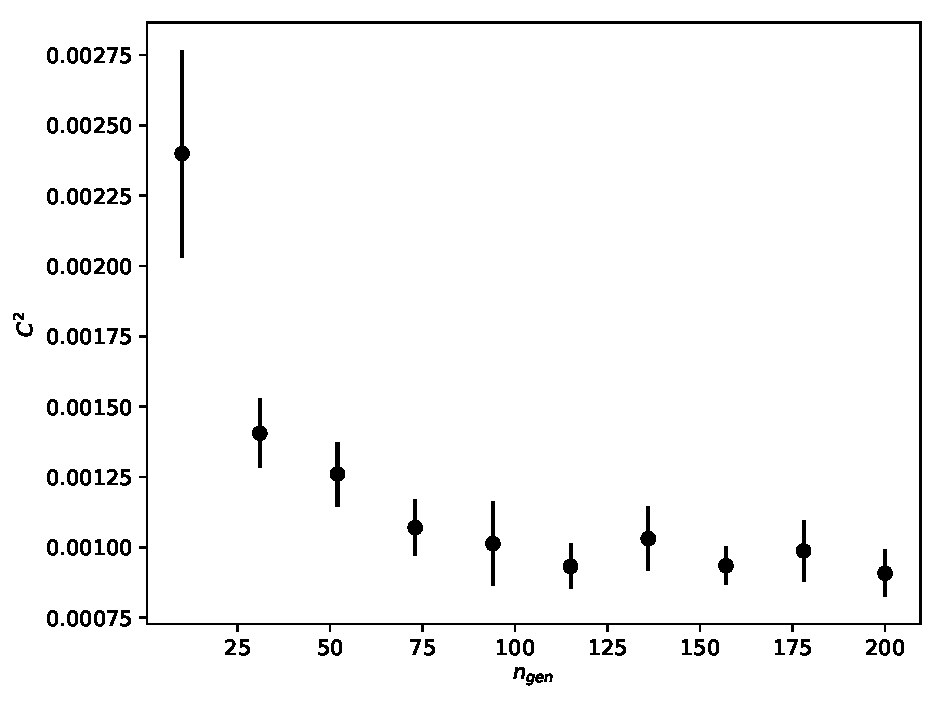
\includegraphics[width=0.9\linewidth,keepaspectratio]{fig/contributions/doe/conv_C2-Ngen-Kdoe2-40.pdf}
\caption{Convergence of the $C^2$-discrepancy function of $n_{gen}$ the size of sample using Metropolis-Hasting for $X_2^{40}$.}
\label{fig:conv-ngen}
\end{figure}


% TODO also good for multifidelity designs


% TODO property A, B with star. Do plot

%\newpage
\section{Results}\label{sec:results}

\subsection{Uniformity of the Design}
As stated previously, the uniformity of the DoE is paramount to ensure that the physics of interest are well captured. \Cref{fig:conv-dim-ns} presents a convergence study of the KDOE method versus \emph{Sobol'} sequences~\citep{Sobol1967}, classical LHS~\citep{Mckay1979}, and optimized LHS as proposed in~\citep{Baudin2015a}. Each point corresponds to a given sample size $N_s$ for a given number of dimensions $n_{dim}$. Due to the stochastic nature of the LHS algorithms and of the KDOE, confidence intervals are computed based on 100 realizations. To measure the improvement of a method with respect to one another, the $C^2$-discrepancy is used~\citep{Fang2006,Androulakis2016} and values are normalized by crude \emph{Monte Carlo} results. This transformation shows that a uniform improvement factor is obtained in comparison to MC. Looking for instance at $n_{dim} = 20$, LHS enables a 20\% improvement in terms of $C^2$-discrepancy over MC, \emph{Sobol'} sequence gives 30\% and both OLHS and KDOE roughly give 40\%.

Looking only at the contestants' methods, their hierarchy is quite stable. OLHS is the best method followed by \emph{Sobol'} sequence and finally LHS. For KDOE, it performs closely to \emph{Sobol'} sequence up to $n_{dim} \lesssim 20$. For $n_{dim} \gtrsim 20$, KDOE performs better than the other methods tested. Moving on to the standard deviation at $2\sigma$ ---\thinspace see~\cref{fig:conv-dim-ns_err}\thinspace---, the variation of the $C^2$-discrepancy is contained between LHS’s and OLHS’s.

\newpage
\begin{figure}[!h]               
\centering
\subfloat[]{
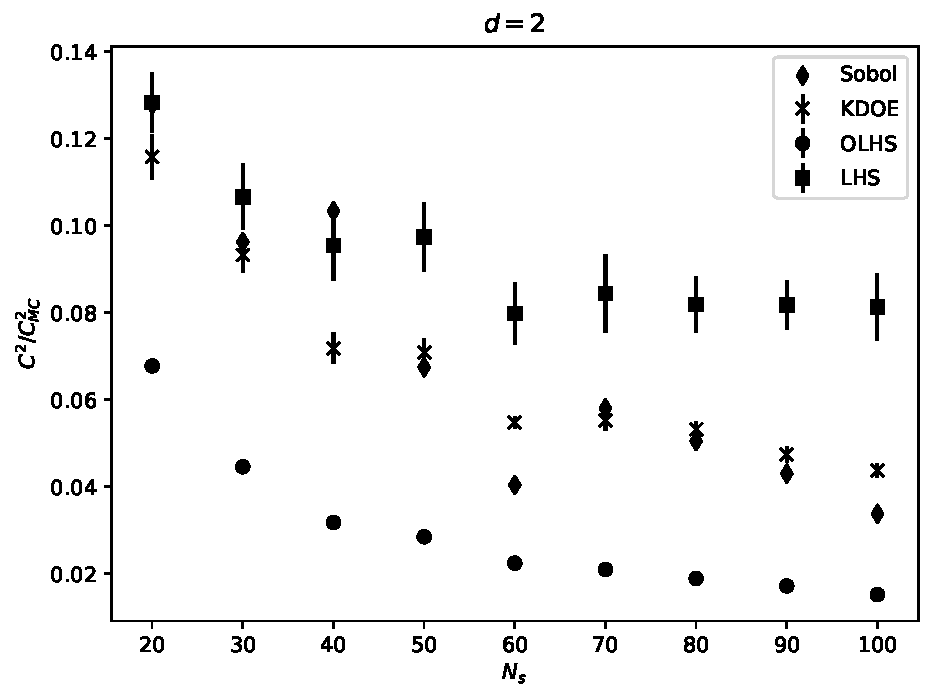
\includegraphics[width=0.48\linewidth,height=\textheight,keepaspectratio]{fig/contributions/doe/kde_2_C.pdf}}
 ~       
\subfloat[]{
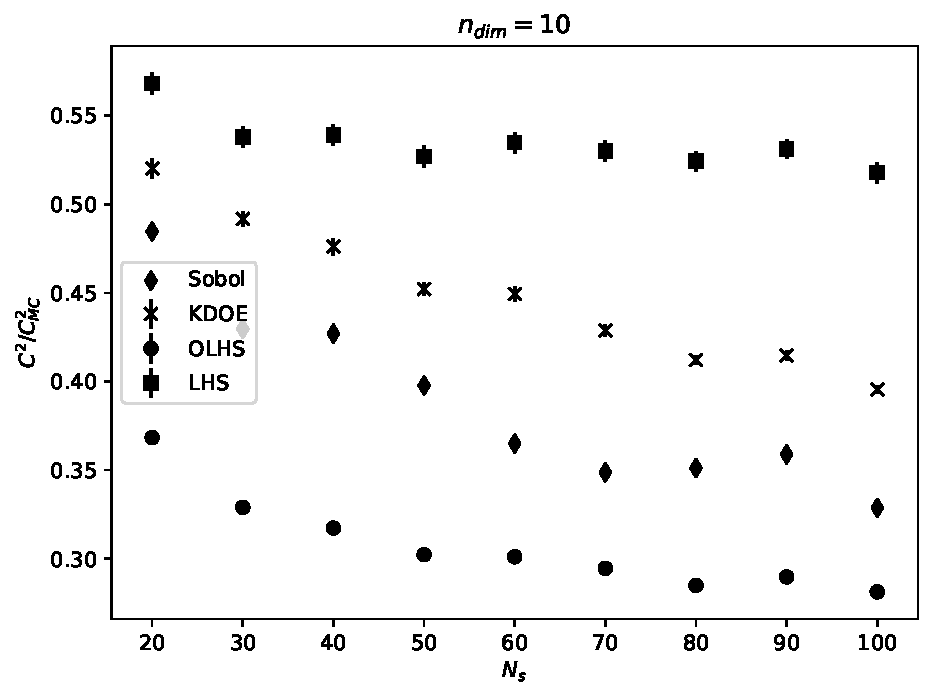
\includegraphics[width=0.48\linewidth,height=\textheight,keepaspectratio]{fig/contributions/doe/kde_10_C.pdf}}

\subfloat[]{
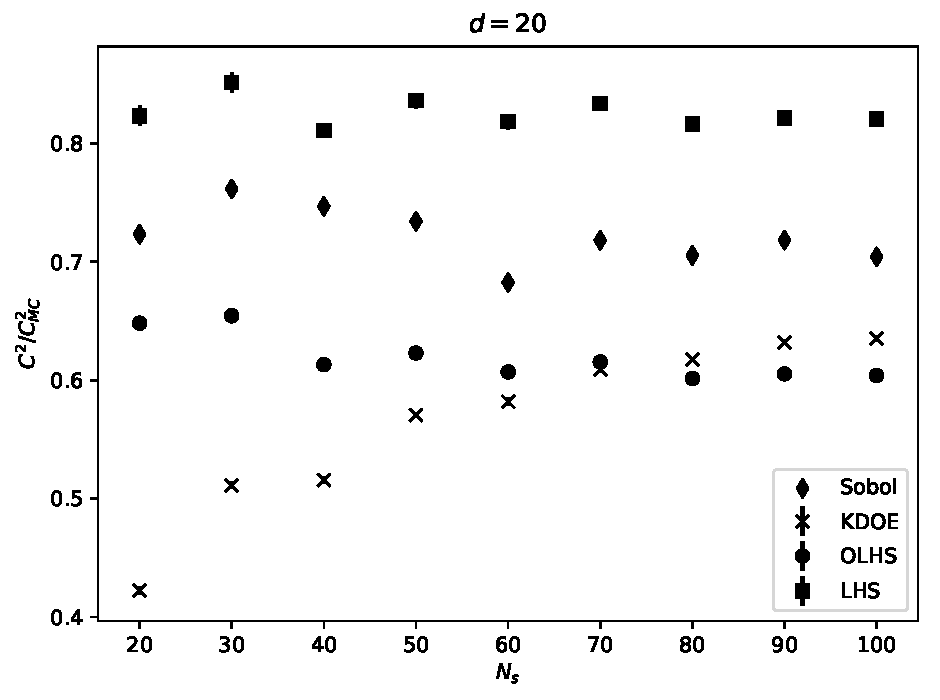
\includegraphics[width=0.48\linewidth,height=\textheight,keepaspectratio]{fig/contributions/doe/kde_20_C.pdf}}
 ~       
\subfloat[]{
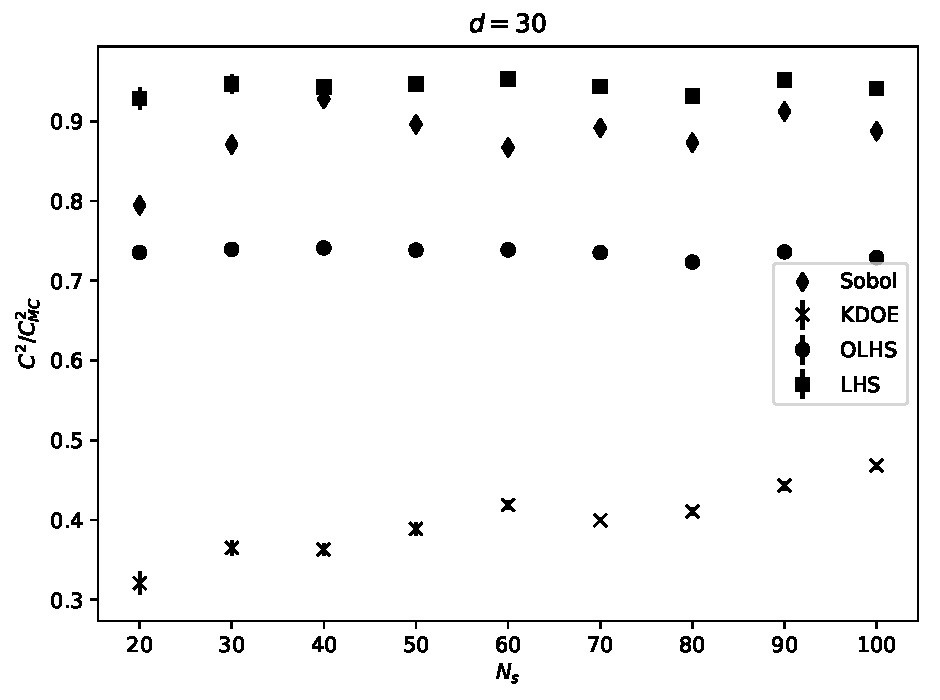
\includegraphics[width=0.48\linewidth,height=\textheight,keepaspectratio]{fig/contributions/doe/kde_30_C.pdf}}
\caption{Adimonsionalized $C^2$-discrepancy function of the number of dimensions $n_{dim}$ of the parameter space and of the size $N_s$ of the design for various DoE methods.}
\label{fig:conv-dim-ns}
\end{figure}
\begin{figure}[!h]               
\centering
\subfloat[]{
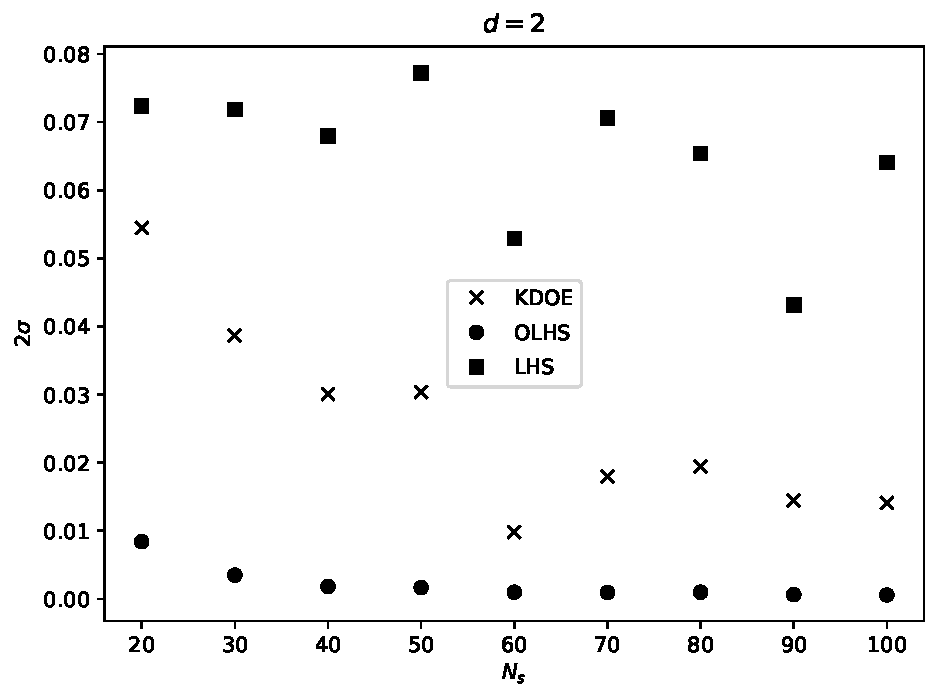
\includegraphics[width=0.48\linewidth,height=\textheight,keepaspectratio]{fig/contributions/doe/kde_err_2_C.pdf}}
 ~       
\subfloat[]{
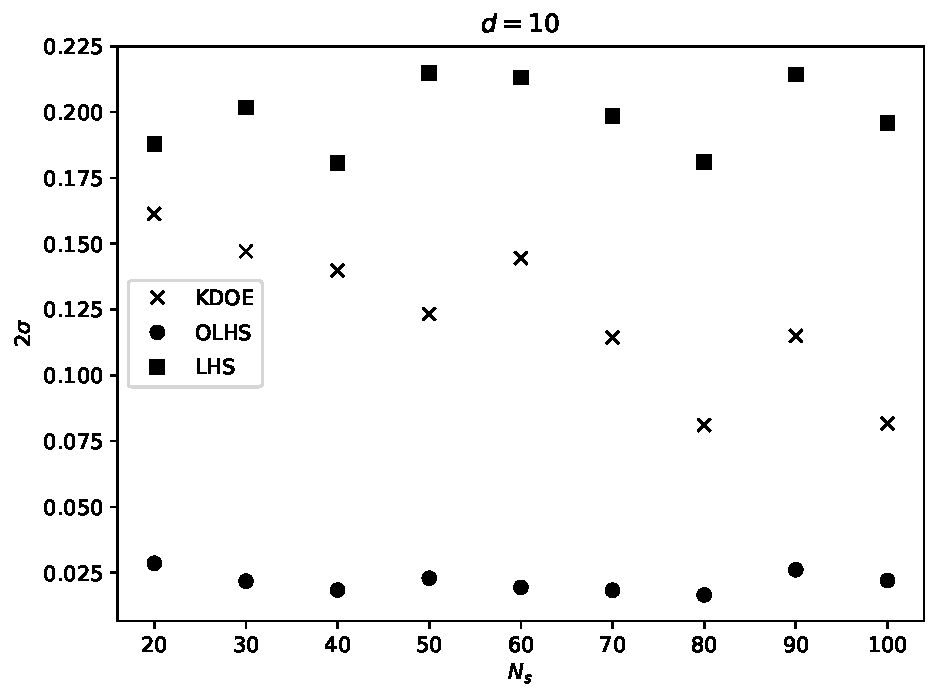
\includegraphics[width=0.48\linewidth,height=\textheight,keepaspectratio]{fig/contributions/doe/kde_err_10_C.pdf}}

\subfloat[]{
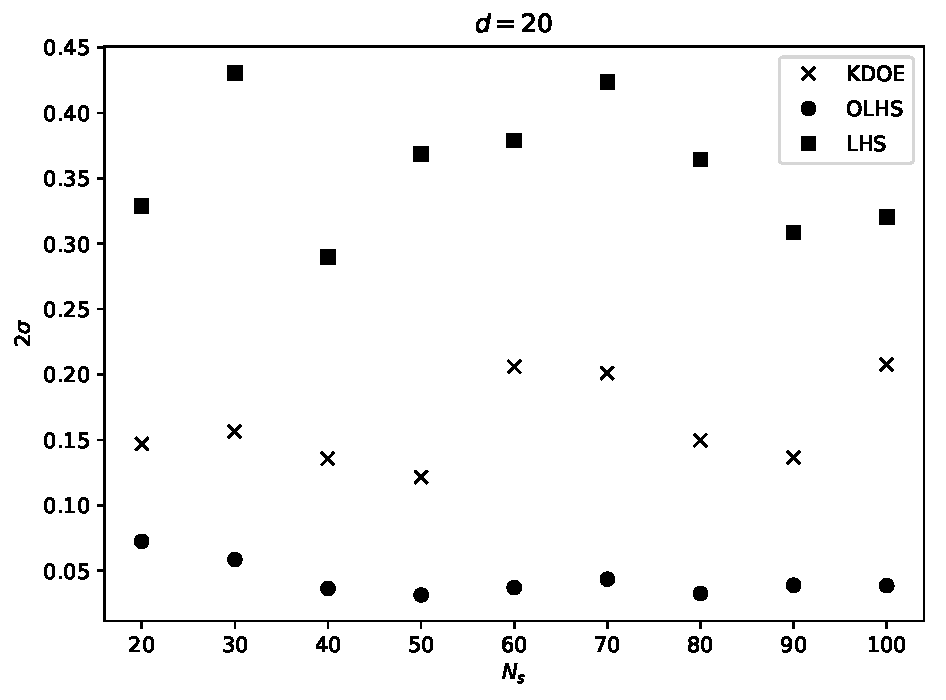
\includegraphics[width=0.48\linewidth,height=\textheight,keepaspectratio]{fig/contributions/doe/kde_err_20_C.pdf}}
 ~       
\subfloat[]{
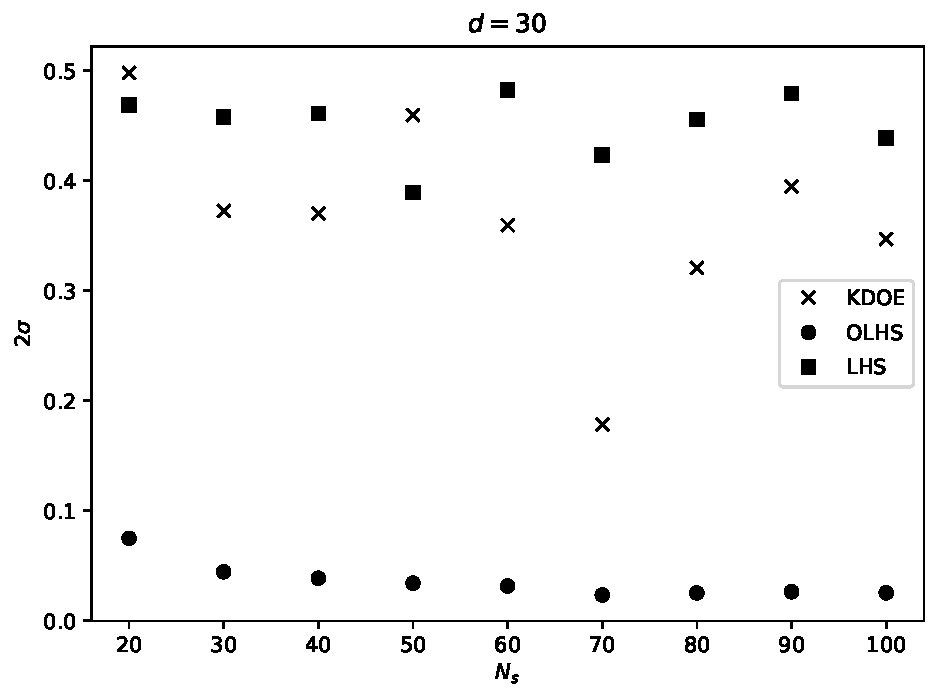
\includegraphics[width=0.48\linewidth,height=\textheight,keepaspectratio]{fig/contributions/doe/kde_err_30_C.pdf}}
\caption{Adimonsionalized $2\sigma$ deviation on the $C^2$-discrepancy function of the number of dimensions $n_{dim}$ of the parameter space and of the size $N_s$ of the design for various DoE methods.}
\label{fig:conv-dim-ns_err}
\end{figure}

\newpage


\Cref{fig:conv-dim-100} presents the convergence analysis of the $C^2$-discrepancy as function of the number of dimensions for $N_s = 100$. When the dimensionality increases, the gain with both LHS and \emph{Sobol'} sequences is close to zero. On the contrary, OLHS seems to stabilize around a 30\% improvement. Regarding KDOE, it performs equally with other methods up to $n_{dim} \lesssim 20$, while for $n_{dim} \gtrsim 20$ it becomes more performant. It can be seen that the method has yet to converge at $n_{dim} = 40$.

\begin{figure}[!h]
\centering
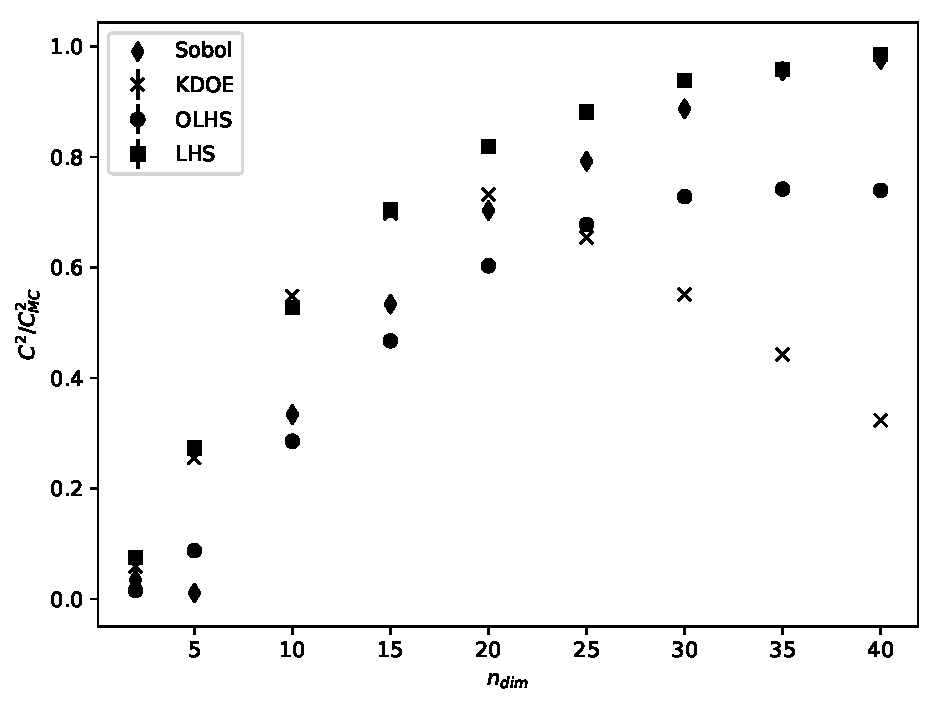
\includegraphics[width=0.9\linewidth,keepaspectratio]{fig/contributions/doe/kde_dim.pdf}
\caption{Adimonsionalized $C^2$ discrepancy function of the number of dimensions $n_{dim}$ of the parameter space with a design of size $N_s = 100$ for various DoE methods.}
\label{fig:conv-dim-100}
\end{figure}

In terms of $C^2$-discrepancy, KDOE appears to perform better with respect to crude \emph{Monte Carlo}, LHS, OLHS and \emph{Sobol'} sequence. \Cref{fig:comp-subspace} shows an example of a sample of size $N_s = 50$ in dimension $n_{dim}=30$. The subprojection $x_{20}/x_8$ is represented. \Cref{fig:comp-subspace}(d) depicts the principal challenge with classical \emph{Sobol'} sequences. In high dimensional parameter space, clear patterns may appear in some subprojections. This behaviour was not observed with KDOE. In this case, the result of the KDOE may not appear optimized for 2-dimensional subprojections. This is due to the fact that the objective is to optimize the total discrepancy of the parameter space.

%C^2\left(\mathbf{X}^{N_s}_{d}
\begin{figure}[!h]               
\centering
\subfloat[KDOE---$C^2=2.18$]{
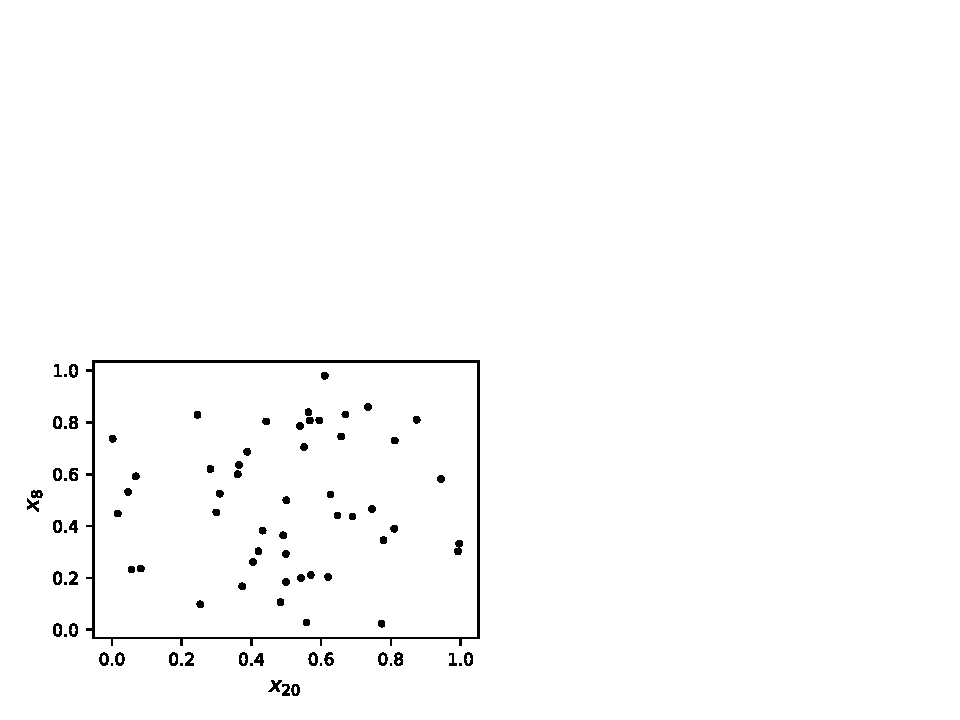
\includegraphics[width=0.47\linewidth,height=\textheight,keepaspectratio]{fig/contributions/doe/20_8_kde.pdf}}
 ~       
\subfloat[OLHS---$C^2=3.43$]{
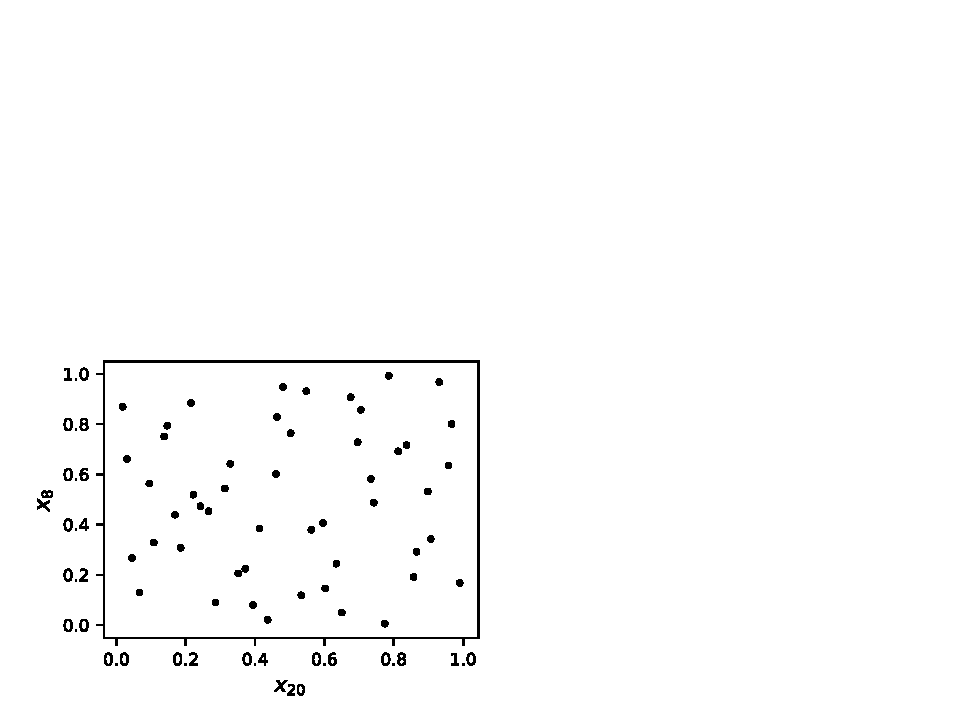
\includegraphics[width=0.47\linewidth,height=\textheight,keepaspectratio]{fig/contributions/doe/20_8_olhs.pdf}}

\subfloat[LHS---$C^2=3.81$]{
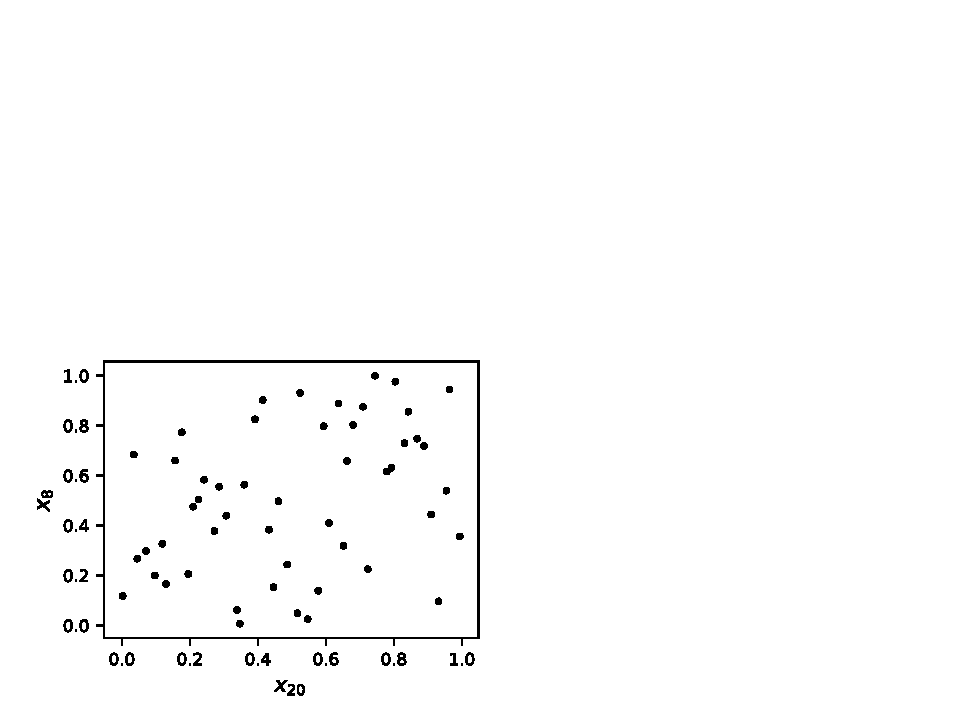
\includegraphics[width=0.47\linewidth,height=\textheight,keepaspectratio]{fig/contributions/doe/20_8_lhs.pdf}}
 ~       
\subfloat[Sobol'---$C^2=3.76$]{
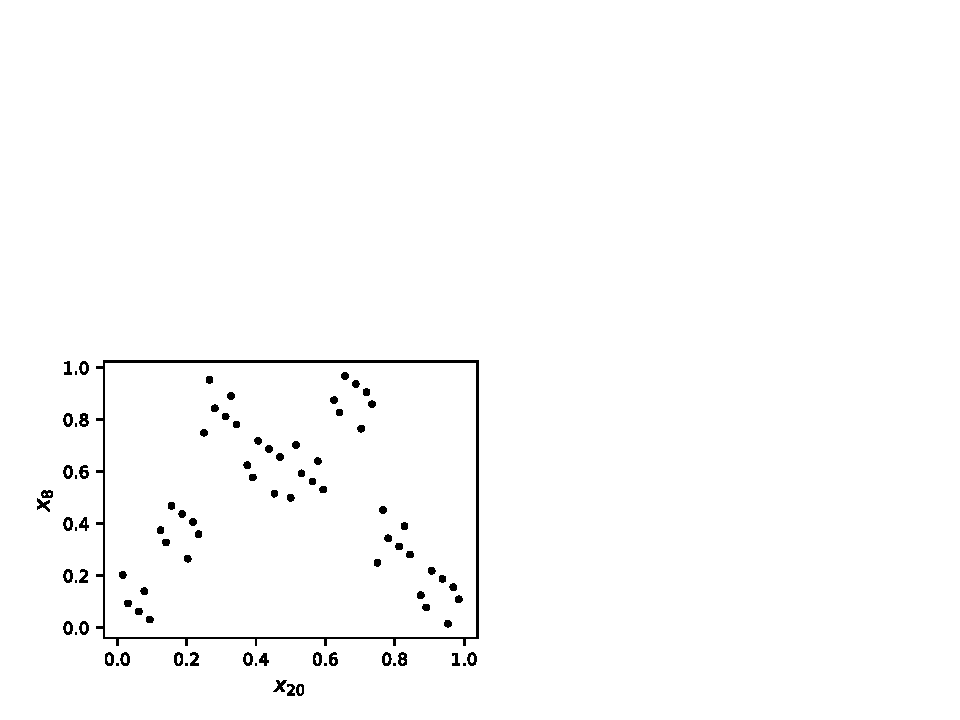
\includegraphics[width=0.47\linewidth,height=\textheight,keepaspectratio]{fig/contributions/doe/20_8_sobol.pdf}}
\caption{Example of a 2-dimensional subprojection of the sample of size $N_s=50$ in dimension $n_{dim}=30$.}
\label{fig:comp-subspace}
\end{figure}


\subsection{Integration Convergence}

Even if this method is not designed for integral evaluation, its performance is evaluated on small numbers of samples up to 512. The number of evaluations has been restricted as the purpose of the method is to generate a small design in high dimensions. Also, the use of an iterative method to generate such sample can be questioned due to the resulting computational cost. Moreover, although this method can be used to continue an existing design created using another technique, such possibility was not evaluated in the following. In~\citep{Kucherenko2015}, convergence plots are presented in order to assess the performance of \emph{Sobol'} sequence versus LHS and \emph{Monte-Carlo} sampling. The functions used are categorized into types A, B and C. These categories state how the variables are important with respect to the function output:
\begin{description}
\item[Type A:] Functions with a low number of important variables,
\item[Type B:] Functions with almost equally important variables but with low interactions with each other,
\item[Type C:] Functions with almost equally important variables and with high interactions with each other.
\end{description}
Type C functions represent the most challenging case. In this work, one function per group is considered as detailed in~\cref{tab:conv_int}. The theoretical integral for all these function in the unit hypercube is 1. Quality of the integration is computed using the Root Mean Square Error (RMSE) defined as
\begin{align}
\epsilon = \left( \frac{1}{K} \displaystyle \sum_{k=1}^{K} \left(I[f] - I_{N_s}^k [f]\right)^2 \right)^{1/2},
\end{align}
\noindent with $K=50$ the number of independent trials and the estimate integral defined as
\begin{align}
I_{N_s}^k [f] = \frac{1}{N_s} \sum_{i=1}^{N_s} f(\mathbf{X}^{i}_d),
\end{align}
\noindent with $f$ the function to integrate. %In each case, the RMSE's evolution is approximated by $cN_s^\alpha$, with $0 < \alpha < 1$ the rate of convergence.

\begin{table}[!h]
\centering
\caption{Type A, B and C functions used in the convergence analysis.}
\begin{tabular}{clc}
\toprule
Type &  Function $f(x)$ & Dim $n$\\
 &   &  \\
\midrule % \cmidrule{2-3}
A & $\displaystyle\prod_{i=1}^n \frac{\mid 4x_i - 2 \mid + a_i}{1 + a_i}$& 30\\
B & $\displaystyle\prod_{i=1}^n \frac{n-x_i}{n-0.5}$ & 30\\
C & $2^n \displaystyle\prod_{i=1}^n x_i$ & 10\\
\bottomrule
\end{tabular}
\label{tab:conv_int}
\end{table}

%\begin{table}[!h]
%\centering
%\caption{Convergence results for type A, B and C functions.}
%\begin{tabular}{clccccc}
%\toprule
%Type &  Function $f(x)$ & Dim $n$ & \multicolumn{4}{c}{Slope $\alpha$} \\
% &   &  & MC & LHS & \emph{Sobol'} & KDOE\\
%\midrule % \cmidrule{2-3}
%A & $\displaystyle\prod_{i=1}^n \frac{\mid 4x_i - 2 \mid + a_i}{1 + a_i}$ & 30 & 0.55 & 0.55 & 0.42& 0.42\\
%B & $\displaystyle\prod_{i=1}^n \frac{n-x_i}{n-0.5}$ & 30 & 0.48& 0.66& 0.46& 0.72\\
%C & $2^n \displaystyle\prod_{i=1}^n x_i$& 10 & 0.47& 0.47& 0.31& 0.39\\
%\bottomrule
%\end{tabular}
%\label{tab:conv_int}
%\end{table}

\Cref{fig:conv_int} presents the convergence study. KDOE is not the best method but seems to compare to both LHS and \emph{Sobol'} sequence. The convergence rates are correct for every function type.


\begin{figure}[!h]               
\centering
\subfloat[Type A]{
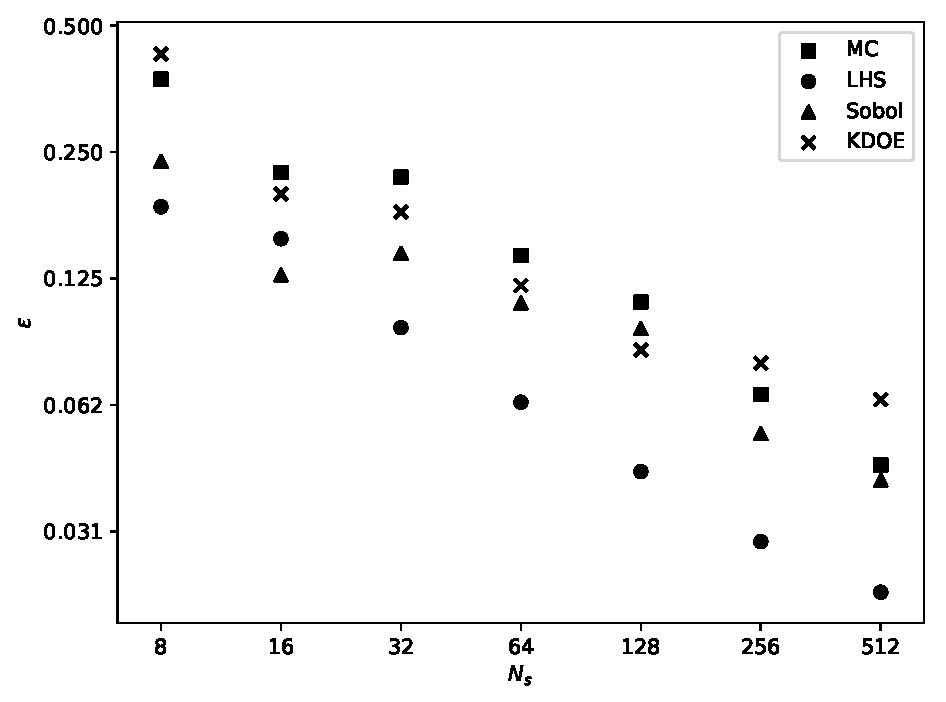
\includegraphics[width=0.6\linewidth,height=\textheight,keepaspectratio]{fig/contributions/doe/kde_int_2A.pdf}}
   
\subfloat[Type B]{
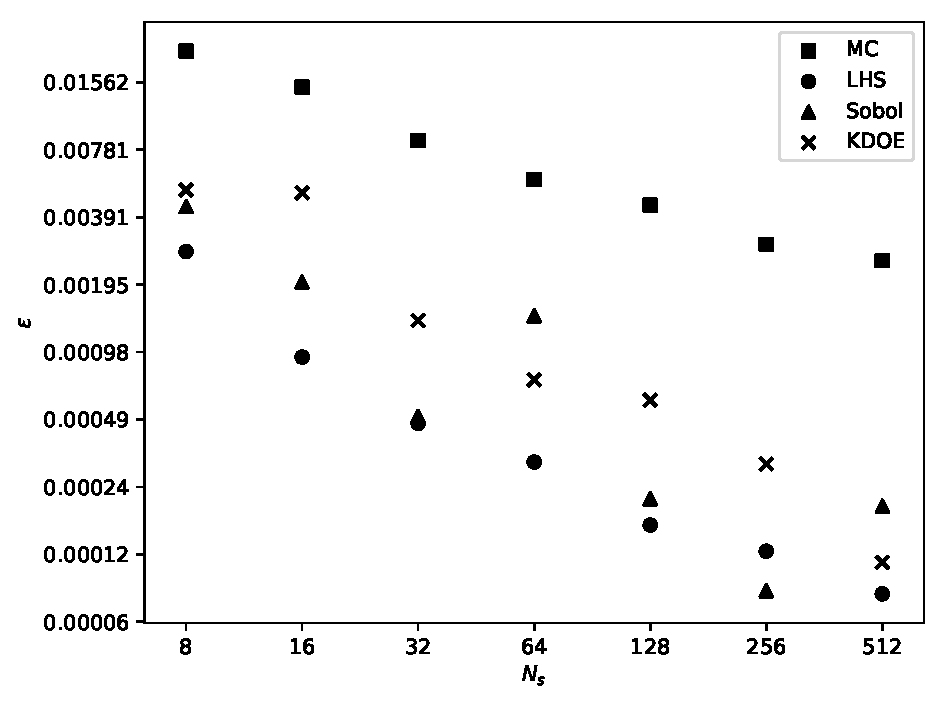
\includegraphics[width=0.6\linewidth,height=\textheight,keepaspectratio]{fig/contributions/doe/kde_int_1B.pdf}}

\subfloat[Type C]{
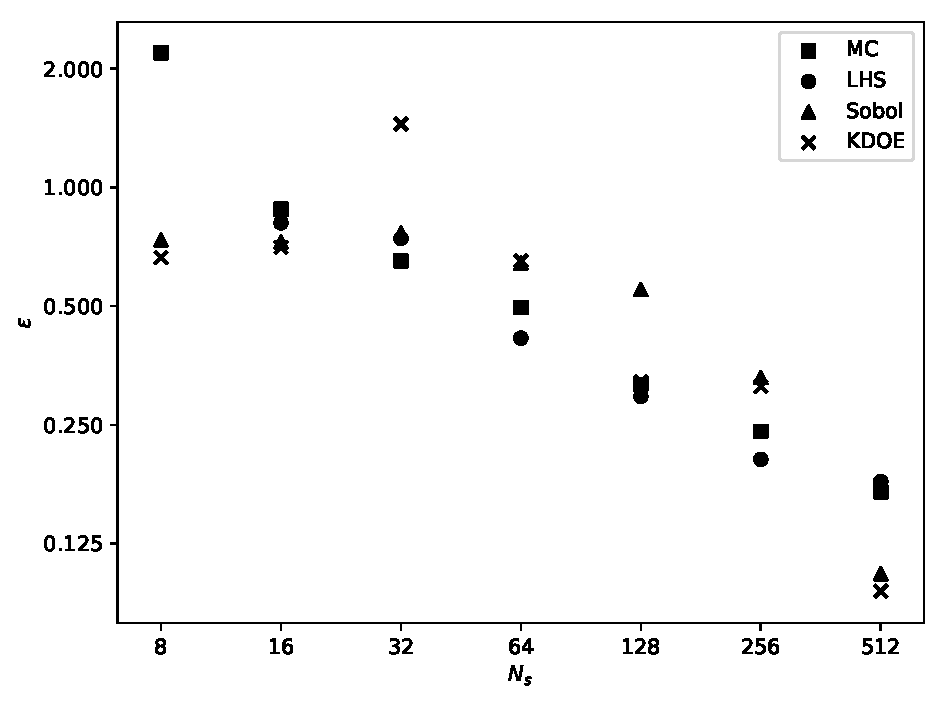
\includegraphics[width=0.6\linewidth,height=\textheight,keepaspectratio]{fig/contributions/doe/kde_int_2C.pdf}}
\caption{RMSE function of the sample size $N_s$ for type A, B and C functions. The trend line corresponds to the RMSE evolution for Monte Carlo's method.}
\label{fig:conv_int}
\end{figure}

\cleardoublepage

\section{Perspectives}

Depending on the property sought, the combination of a Kernel and a metric allows an infinite customization of the method.

Using the Minkowsky distance as a metric, the LHS constrain is not strict which can be useful when dealing with discrete parameters. Indeed, strict LHS would prevent having more than one sample per discreet parameter. In~\cref{fig:lhs_const}(a), an additional constrain is added to strongly limit the probability to 0 when the $L_{-\infty}$-norm is inferior to a threshold. This limitation can be restricted to a domain of influence using an additional $L_2$-norm constrain (\cref{fig:lhs_const}(b)). Hence, this method acts as an iterative LHS strategy.

\begin{figure}[!h]               
\centering
\subfloat[Inverse Mindkowsky distance with LHS properties]{
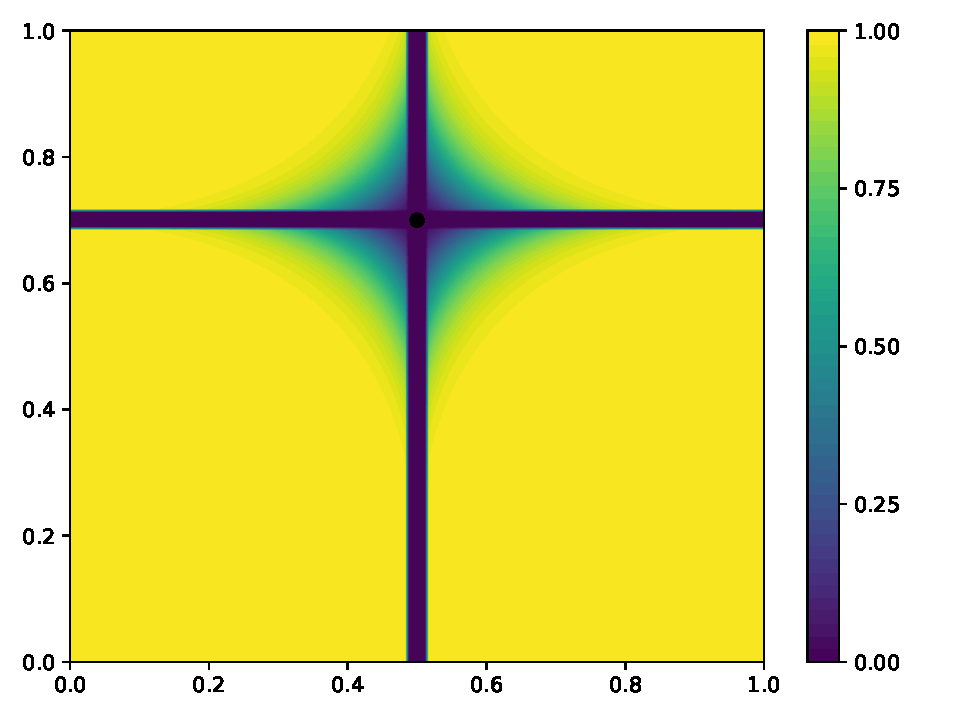
\includegraphics[width=0.49\linewidth,height=\textheight,keepaspectratio]{fig/contributions/doe/kde_minkowsky_LHS.pdf}}
~
\subfloat[Inverse Mindkowsky distance with LHS properties and constrain]{
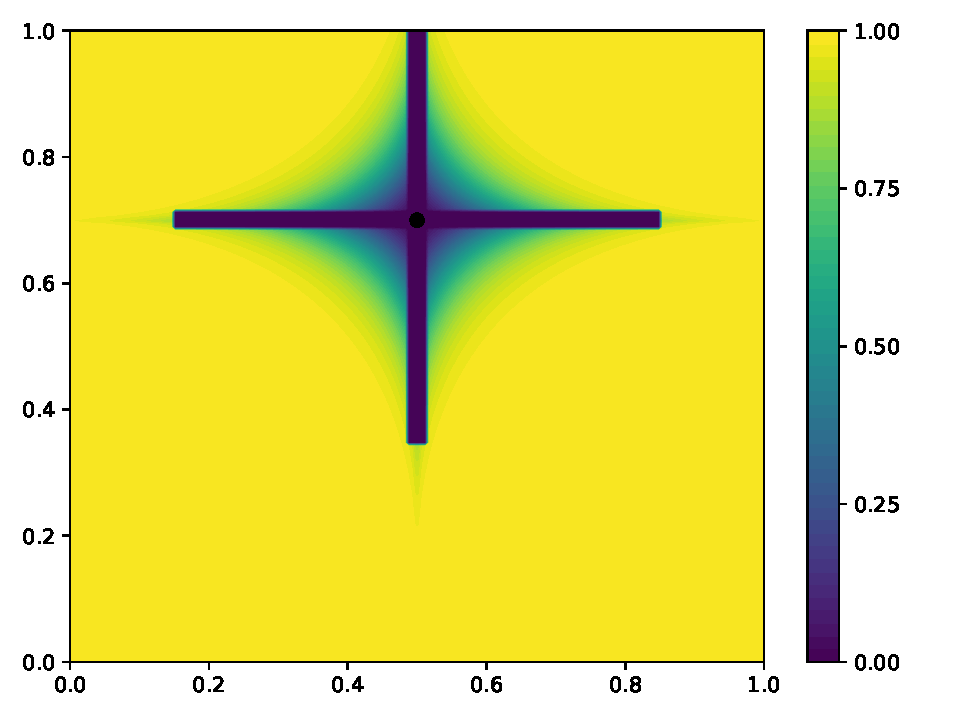
\includegraphics[width=0.49\linewidth,height=\textheight,keepaspectratio]{fig/contributions/doe/kde_minkowsky_LHS-const.pdf}}

\caption{Probability density in a 2-dimensional parameter space. \emph{Dot} represents the sample used to fit the KDE.}
 \label{fig:lhs_const}
\end{figure}

%\begin{figure}[!h]
%\centering
%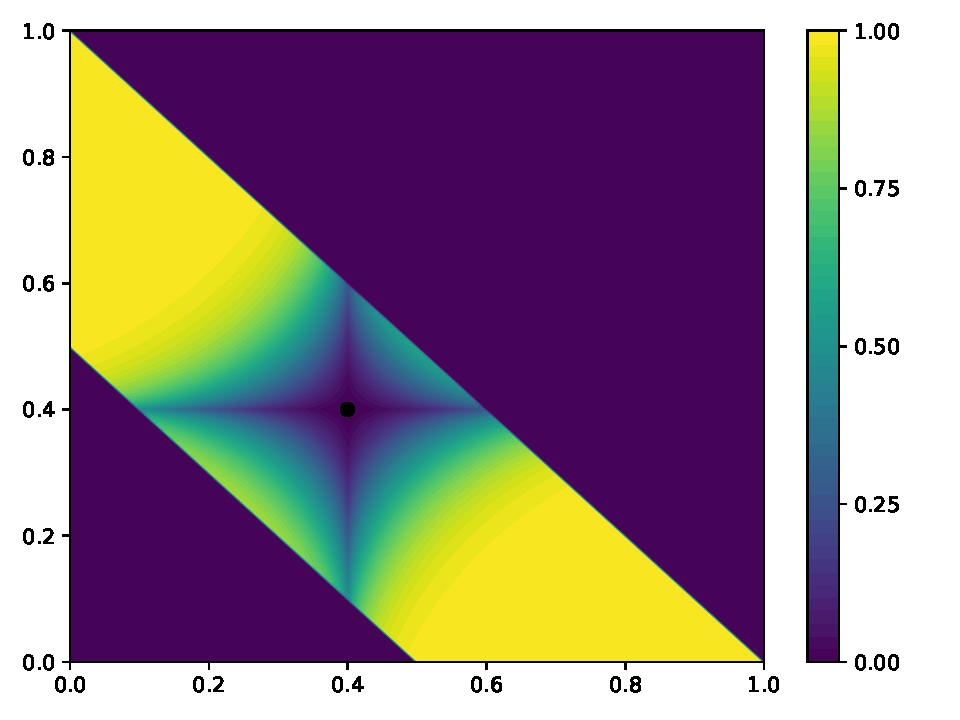
\includegraphics[width=0.9\linewidth,keepaspectratio]{fig/contributions/doe/kde_constrain.pdf}
%\caption{Probability density in a non-rectangular 2-dimensional parameter space. \emph{Dot} represents the sample used to fit the KDE.}
%\label{fig:const_kde}
%\end{figure}


Using this method, it is also possible to consider non-rectangular domains~\citep{Lekivetz2015}. This example presents a 2-dimensional domain with the constrain $0.5 < x_1 \times x_2 < 1$. In this case, the selection of the point criterion has to be changed as the $C^2$-discrepancy assumes rectangular domains. \Cref{fig:constrain} shows a sampling of the aforementioned constrained design using a \emph{maximin} criterion~\citep{Fang2006}. This criterion only considers the points of the sample resulting in an optimal sphere packing problem. The criterion seeks to maximize the minimal distance between the new point and the existing samples. This adaptation is to ensure that the new point is not penalized by existing samples that would be ill positioned in the parameter space.

\begin{figure}[!h]
\centering
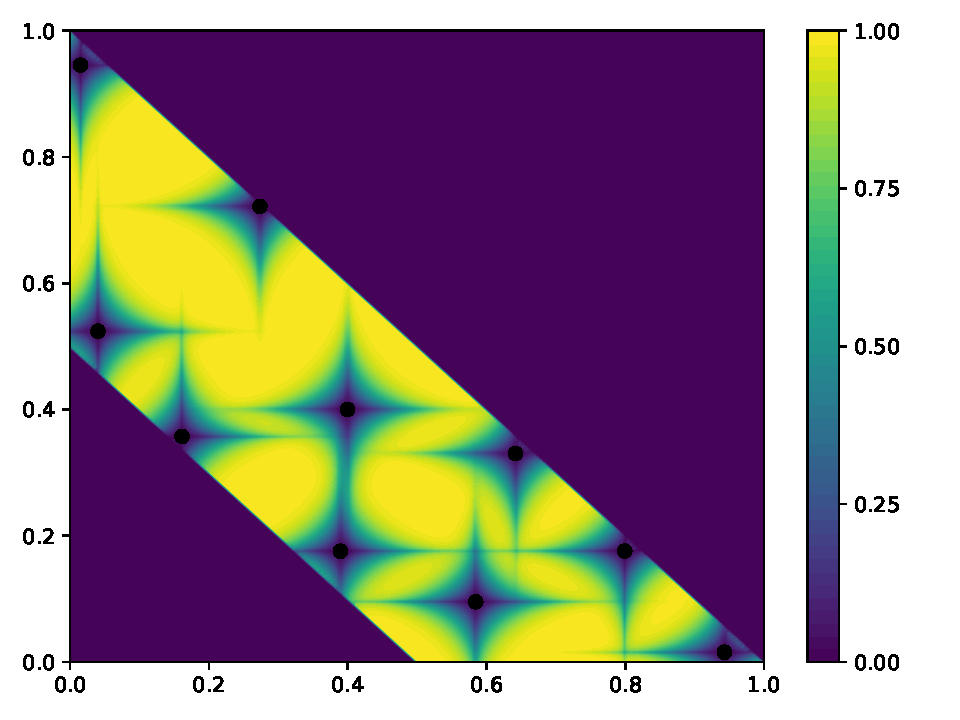
\includegraphics[width=0.9\linewidth,keepaspectratio]{fig/contributions/doe/10_star_constrain.pdf}
\caption{Probability density in a non-rectangular 2-dimensional parameter space. The 10 \emph{dots} represent the samples used to fit the KDE.}
\label{fig:constrain}
\end{figure}

The ability to change the selection criterion is even more useful. With a prior knowledge on the sensitivity of the parameters to the quantity of interest~\citep{Saltelli2007}, it is possible to bias the design. Considering a 2-dimensional space ---\thinspace as the example in~\cref{fig:sensitivity}\thinspace---, if the parameter $x_2$ is known to have a small impact, it might be more interesting to optimize the $C^2$-discrepancy on the parameter $x_1$. More complicated things can be performed if one wants to optimize a particular subprojection as in~\citep{Joseph2015}. This is referred to as \emph{Maximum Projection Design}.

\begin{figure}[!h]
\centering
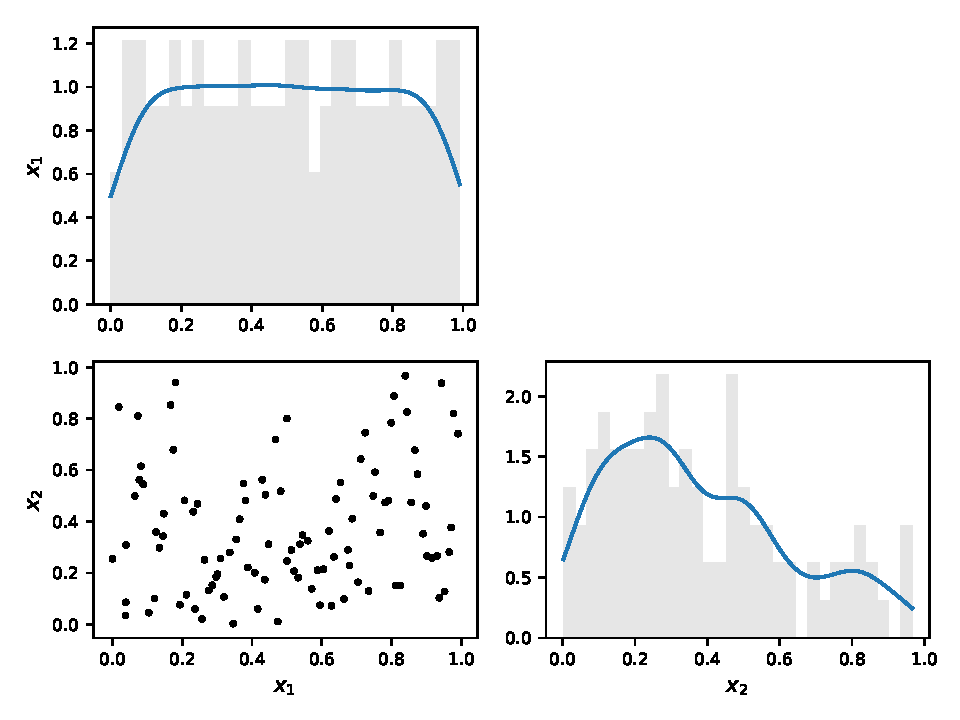
\includegraphics[width=0.9\linewidth,keepaspectratio]{fig/contributions/doe/kde_sensitivity.pdf}
\caption{2-dimensional parameter space with $x_0$ the highest . \emph{Dots} represent the sample. Sample distributions for each parameter are plotted along the diagonal.}
\label{fig:sensitivity}
\end{figure}

Last but not least, this method can be used to generate designs by mixing continuous and discrete variables. The star shape of the kernel does not forbid the presence of a new sample along a given axis, it lower its probability of being sampled up to a certain distance. In this case, a Gaussian kernel might be more appropriate in order to relax some constrains on the axes. Another option would be to modify the kernel to limit the point influence along the discrete axis.

The ability to play both with the kernel and the selection criteria is really powerful as it allows to manage most of the challenges in constrained optimization problems, use sensitivity information, and sample by means of following individual PDFs for each parameter.

\section{Conclusion}
% 1. Novelty of the results
This work proposes a new method to stochastically and iteratively sample a parameter space, referred to as KDOE method. This is a two-step process: \emph{(i)} through a Kernel Density Estimation (KDE) some candidates are generated, then \emph{(ii)} the best candidate is selected based on a criterion. This method does not take into account the physics of the problem of interest as adaptative strategies, but is purely iterative and case independent.

% 2. Local, specific, scientific benefits
Compared to LHS and low discrepancy sequences, KDOE is totally iterative and stochastic. The space-filling properties of the new designs based on the $C^2$-discrepancy are assessed and show good behaviour in high dimensions with small sample sizes. Moreover, it showed similar capabilities for numerical integration compared to classical methods.The KDOE method is versatile in the sense that it can be easily adapted to take into account constrains in the parameter space, both discrete and continuous parameters can be used and sensitivity indices of the parameters can be incorporated. This ability comes from the two-step process which can be independently tuned.

% 3. Global, societal, general benefits
The quality of the design is of prime importance as it determines the quality of the analysis of the experiments. The proposed method provides an alternative to classical one-shot methods to generate initial designs and to continue existing ones. Its versatility and performance allow the analysis of expensive and high-dimensional cases to be within affordable budgets.


\chapter{Resampling the Design of Experiments}
\section{Introduction}

The accuracy of an uncertainty quantification being directly correlated to the quality of the surrogate~\cite{iooss2010}, the present work aims at improving its construction by using two new strategies for resampling the parameter space. The presented techniques show an improvement of the predictive quality of the model with high dimensional analytical input functions. An industrial application is targeted, the aerothermal flow around the \textit{LS89}~\cite{arts1990}. An Uncertainty Quantification study has already been performed using Reynolds Averaged Navier-Stokes (RANS)~\cite{Gourdain2010,emory2016} but the first UQ analysis using Large Eddy Simulation (LES) is here presented (see~\cref{chap:ls89}). LES are high-fidelity full 3D unsteady simulations. This approach comes at a high CPU cost which requires the use of High Performance Computing (HPC) resources.

\section{Presentation of the methods}

Aside from sequence designs that are intrinsically iterative, all designs can be increased step-by-step through several techniques. A natural way is to optimize the discrepancy or some other criteria such as the entropy or the distance between points~\cite{Fang2006}. These kinds of methods only take advantage of the position of the points in the parameter space. The expected quality of such method is, as expected (and from our testing, not presented in this work), at best close to a low discrepancy sequence. A complementary strategy consists in exploring the space using as few points as possible and then refine the exploration around interesting zones. In the work of~\cite{scheidt2006,braconnier2011}, they used detection of optima, nul gradients and also information about the Gaussian processes variance. This method is denoted hereafter $\sigma$ method. One caveat with crude $\sigma$ method is that points are preferentially added at boundaries of the parameter space. This is further described in~\cref{sec:delta-space}. This behaviour motivates the research of new refinement methods that would use this information without being constrained to boundaries.

Aside from this baseline, two novel strategies---LOO-$\sigma$ and LOO-\textit{Sobol'}---have been developed and are presented in this work. The common strategy is detailed in~\cref{alg:refine}.

\begin{algorithm}
  \caption{Refinement strategy}
  \label{alg:refine}
  \begin{algorithmic}[1]
  \Require $N_{max}$, $threshold$, $\mathcal{M}_{gp}$, $N_s$
%  \Ensure $N_c = \frac{C - N_e}{\alpha}$
% \Comment{a test comment}
  \While{$LOO-quality < threshold$ and $N_s < N_{max}$}
    \State $\mathbf{x}_{L} \gets$ least stable point of the design
    \State $\mathcal{H_{L}} \gets$ hypercube around $\mathbf{x}_{L}$
    \State $\mathbf{x}_o \gets \max \mathbb{V}[\mathcal{M}_{gp}]$, within $\mathcal{H_{L}}$
    \State Compute a new snapshot at $\mathbf{x}_o$
    \State Update pGP surrogate $\mathcal{M}_{gp}(\mathbf{x}_*)$
  \EndWhile
  \end{algorithmic}
\end{algorithm}

Starting from an initial parameter space, the quality of the current model gives the most sensitive point of the design. Around this point, a hypercube is constructed. Within this hypercube the model's variance is maximized which gives a new point. Each strategy is described hereafter:

\begin{itemize}
\item Variance ($\sigma$), \hfill\\
As stated in \cref{sec:GP}, one of the main advantages of Gaussian processes over other surrogates is to provide an insight into the variance of the solution. The first method consists in using this data and weight it with the eigenvalues of the POD:
\begin{align}
\sum_{i=1}^k \lambda_i^2 \times \mathbb{V}[\mathcal{M}_{gp}(\mathbf{x}_*)]_{i}.
\end{align}

Global optimization of this indicator gives the new point to simulate~\cite{wales1997}.

\item Leave-One-Out (LOO) and $\sigma$, \hfill\\
A LOO is performed on the model and highlights the point where the model is the most sensitive. The strategy here is to add a new point around it. The creation of the hypercube is described in \cref{sec:hypercube}. Within this hypercube, a global optimization over $\sigma$ is conduced giving the new point.

\item  LOO-\textit{Sobol'}, \hfill\\
Using the same steps as with the LOO-$\sigma$ method, the hypercube around the point is here truncated using prior information about \textit{Sobol'} total indices---see \cref{sec:uq}. For instance, in a 2-dimensional case if $S_{T_{x_1}} = 0.8, S_{T_{x_2}} = 0.2$, the hypercube will be shrunk by 80\% along $x_1$'s axis and by 20\% along $x_2$'s axis. The algorithm ensures indices to be bounded between 0.1 and 1. This prevents some dimensions to be squashed prematurely. The method requires that indices be close to convergence not to bias the result. However, the bias can be intentional depending on the insight we have about the case. 

\item  Hybrid.\hfill\\
This last method consists of a navigator composed by any combination of the previous methods.
\end{itemize}

The evaluation of the latter composite method is not presented in this work. Although the computation of the LOO metric is merely an attempt to characterize the model's global quality, this mainly serves to assess the surrogate model's stability. If the model's response surface is not affected by the removal of a particular point, it is interpreted as stability---or a non-sensitivity---of the model to this action. This technique aims at stabilizing the model.

\section{Construction of the Hypercube}
\label{sec:hypercube}

To resample locally the parameter space, a hypercube is constructed around point $p$ which is the most sensitive in the construction of the surrogate model---LOO point, see \cref{sec:validation}. An optimization problem is defined to construct the largest hypercube bounded by the surrounding points $\mathcal{P}$ as shown in \cref{fig:hypercube}. This allows to only consider the vicinity of the point.

\begin{figure}[h]
\centering
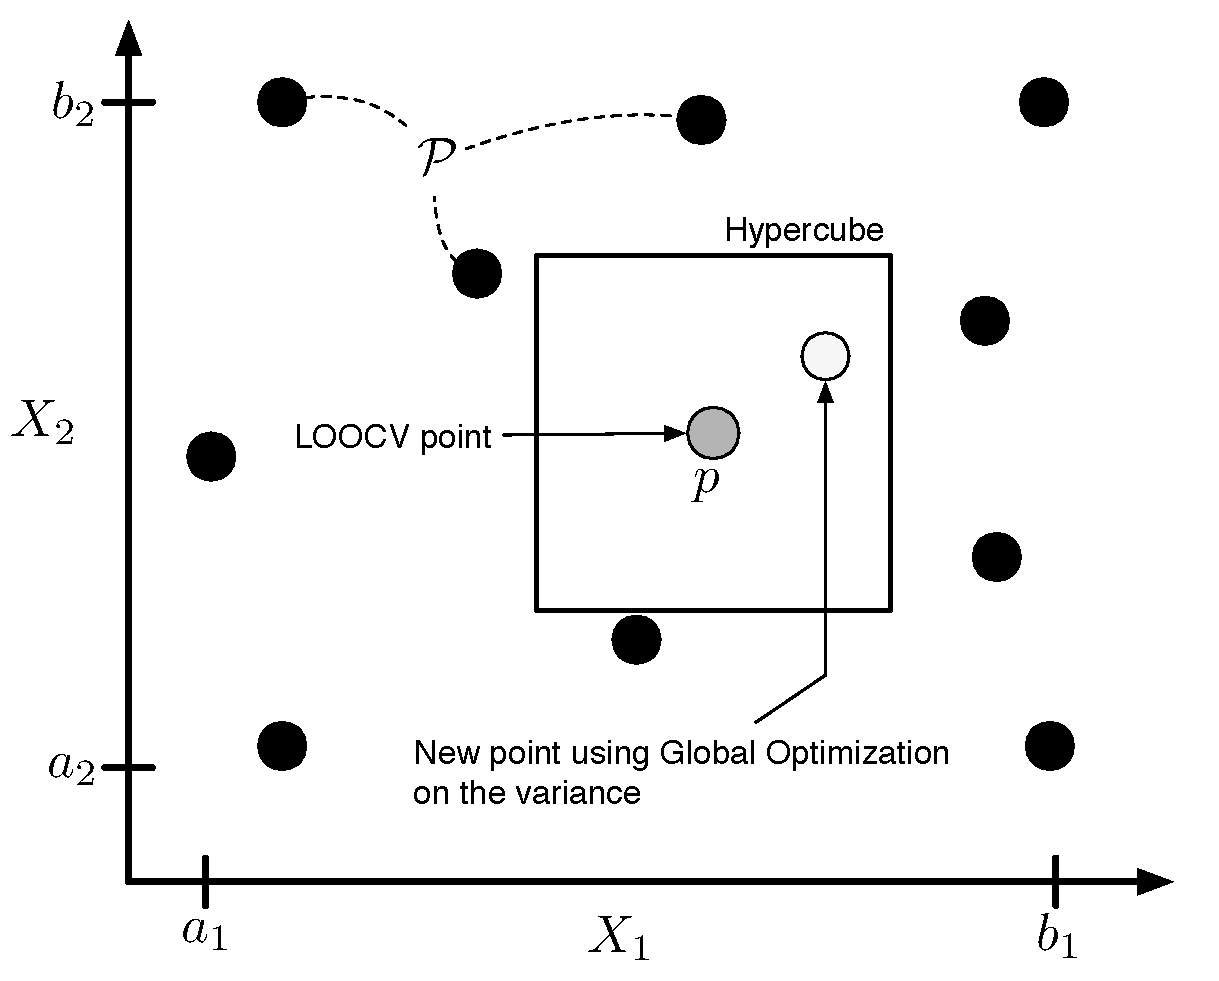
\includegraphics[width=0.8\linewidth,keepaspectratio]{fig/contributions/resample/2_1column_color-online-only_hypercube.pdf}
\caption{Sketch of a hypercube of size $[a_i, b_i]^2$. The grey dot is the LOO point $p$, the black dots are the surrounding points $\mathcal{P}$ and the white dot is the new point to evaluate.}
\label{fig:hypercube}
\end{figure}

The hypercube is defined by the cartesian product of the intervals of the ${n_{dim}}$ parameters \textit{i.e.} $[a_i, b_i]^{n_{dim}}$. The constrained optimization problem consists in finding the coordinates of the hypercube, hence the problem writes
\begin{align}
\left\{\begin{array}{rc} \max  &\parallel (\mathbf{b} - \mathbf{a}) \parallel_{2} \\\mathcal{P} &\notin [a_i, b_i]^{n_{dim}} \\ p &\in [a_i, b_i]^{n_{dim}} \end{array}\right. .
\end{align}
A maximum cube-volume aspect ratio~\cite{smith1998} is also defined in order to preserve the locality. This gives the new constrain
\begin{align}
C : \sqrt[n]{\frac{\max (\mathbf{b} - \mathbf{a})}{\displaystyle\prod_{i = 1}^{n_{dim}} \max (b_i - a_i)}} < \epsilon ,
\end{align}
with $\epsilon = 1.5$, set arbitrarily to prevent too elongated hypercubes. The global optimum is found using a two-step strategy: first, a discrete optimization using $\mathcal{P}$ gives an initial solution; second a basin-hopping algorithm~\cite{wales1997} finds the optimum coordinates of the hypercube.


\section{Results}
\label{sec:results}

The benefits and mechanisms of the methods are first evaluated on complex analytical functions. The chosen functions are defined in~\cref{sec:functions}. Then, the treatment of the parameter space's boundary is presented in~\cref{sec:delta-space}. Taking into account this issue, the analytical functions are tested in~\cref{sec:res-functions}.

\subsection{Analytical functions}
\label{sec:functions}

In order to test the new resampling methods, three analytical functions---see~\cref{tab:functions}---with increasing numbers of input dimensions are presented, namely: \textit{(i)} \textit{Rosenbrock} ; \textit{(ii)} \textit{Ishigami} ; and \textit{(iii)} \textit{g-function}~\cite{molga2005,ishigami1990,Saltelli2007,Legratiet2016}. They are all widely used because they are nonlinear and nonmonotonic. Note that similar results were obtained on other functions. Moreover, two versions of the \emph{g-function} 11-D are assessed. \textit{g-function (i)} 11-D demonstrates the behaviour of the methods whith a small number of input parameters contributing to the QoI, whereas \textit{g-function (ii)} 11-D exhibits more influent input parameters---see~\cref{tab:cv-budget-q2} for \emph{Sobol'} indices.

\begin{table}[h]
\centering
\setcellgapes{5pt}
\makegapedcells
\begin{tabular}{lll}
\toprule
Function&Hypercube & Definition \\
\cmidrule{1-3}
\textit{Rosenbrock} 2-D& $[-2.048, 2.048]^2$ & $
f(X_1, X_2) = \sum_{i = 1}^{d-1}[100(x_{i+1} - x_i^2)^2  +(x_i -1)^2].$\\
\textit{Ishigami} 3-D& $[-\pi, \pi]^3$ & $ f(X_1, X_2, X_3) = \sin X_1 + 7 \sin^2 X_2 + 0.1 X_3^4 \sin X_1. $\\
\textit{g-function} 4-D& $[0, 1]^4$ & $
f(X_1, X_2, X_3, X_4) = \prod_{i=1}^4 \frac{\lvert 4X_i - 2\rvert + a_i}{1 + a_i}, \quad a_{i} = i.$\\
\textit{g-function (i)} 11-D & $[0, 1]^{11}$ & 
$\begin{multlined}[t][0.6\linewidth]
f(X_1, ..., X_{11}) = \prod_{i=1}^{11} \frac{\lvert 4X_i - 2\rvert + a_i}{1 + a_i},\\[-1ex]
\hspace{50pt} \mathbf{a} = [1, 2, 5, 10, 20, 50, 100, 500, 1000, 1000, 1000]\hfill
\end{multlined}$\\
\textit{g-function (ii)} 11-D & $[0, 1]^{11}$ &
$\begin{multlined}[t][0.6\linewidth]
f(X_1, ..., X_{11}) = \prod_{i=1}^{11} \frac{\lvert 4X_i - 2\rvert + a_i}{1 + a_i},\\[-1ex]
\hspace{51pt} \mathbf{a} = [1, 2, 2, 3, 3, 10, 50, 50, 50, 100, 100]\hfill
\end{multlined}$\\
\bottomrule
\end{tabular}
\caption{Analytical functions considered sorted by increasing number of input parameters.}
\label{tab:functions}
\end{table}

\subsection{Restriction of the DoE}
\label{sec:delta-space}

The first step when constructing a model is to define the DoE. This is done by defining the range of each input parameter, the boundaries that describe a hypercube. Then, using a low discrepancy sequence as described in \cref{sec:doe}, an initial pool of snapshots is computed within the hypercube. However, when constructing a model based on Gaussian Process regression, the error is important at the boundaries of the DoE due to the lack of information. The model is thus not able to extrapolate accurately at these locations. If using the variance technique as it is, the algorithm tends to add points around the corners and only after it considers other parts of the domain. When dealing with a low dimensional case---fewer than three parameters as with the \textit{Michalewicz} function which uses two input parameters, see \cref{fig:rs-michalewicz}---, a few iterations are "wasted" in the process.

\begin{figure}[h]
\centering
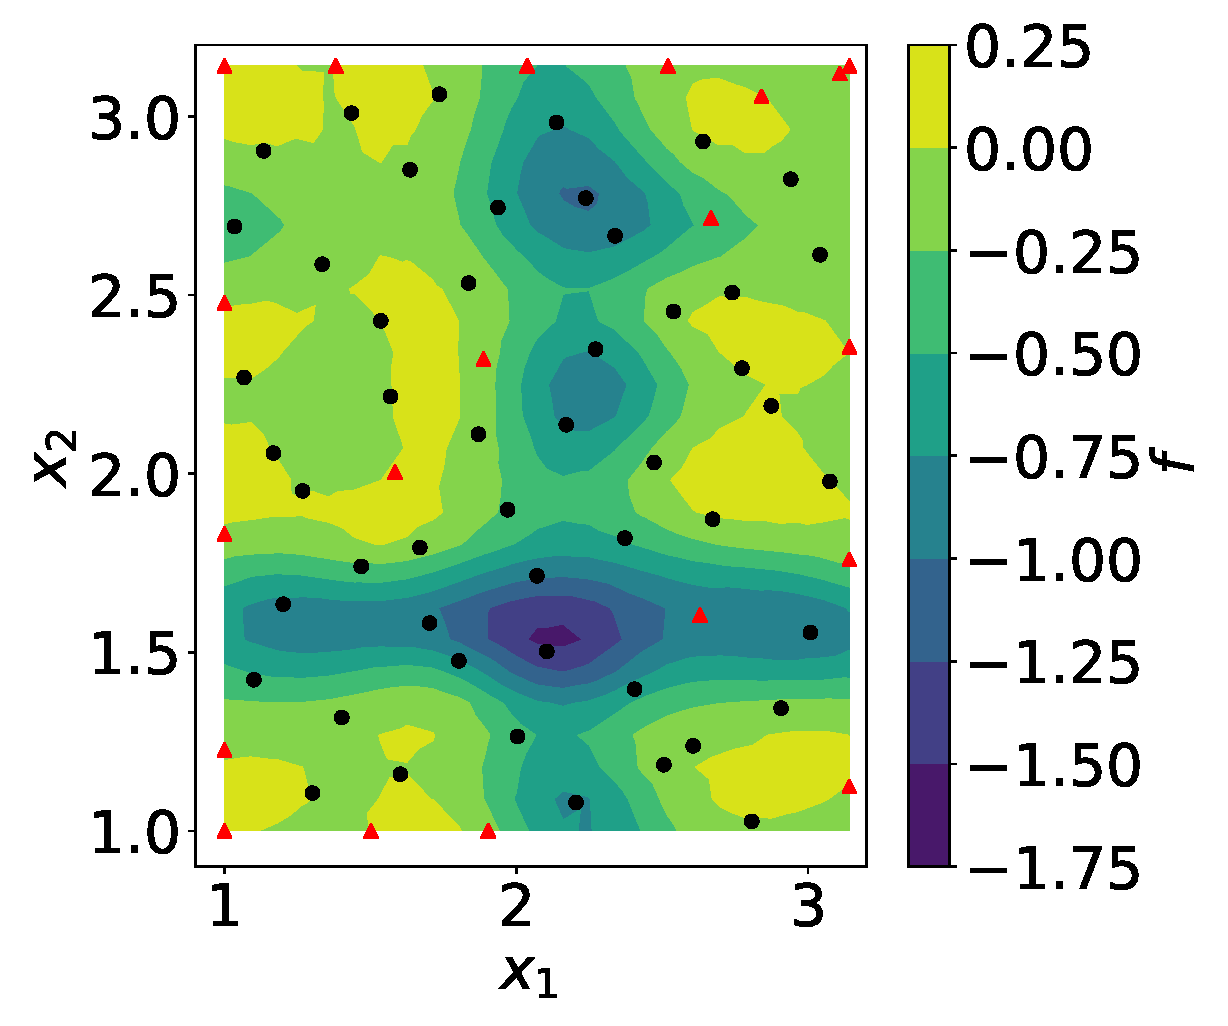
\includegraphics[width=\linewidth,keepaspectratio]{fig/contributions/resample/3_1column_color-online-only_response_Michalewicz_sigma.pdf}
\caption{\textit{Michalewicz} function: dots represent the initial sample of 50 points and diamonds represent the 20 resampled points. The function was evaluated on the hypercube $[1, \pi]^2$}
\label{fig:rs-michalewicz}
\end{figure}

When increasing the number of parameters, there is a larger number of boundaries to cover. This has been confirmed on the \textit{Ishigami} function (3 input parameters) for which the reported $Q_2$ values are even worse. As shown in \cref{tab:size-q2-ishigami}, the optimization process is being over constrained in these regions and the global predictions are degraded. To obtain this Table, the initial sample was increased using a constant number of resampling points (10 points) and the error was measured using a uniform distribution on the domain, confirming the importance of the boundary treatment.

\begin{table}[h]
\centering
\begin{tabular}{lcc}
\toprule
Initial sample&Total size & $Q_2$ \\
\cmidrule{1-3}
30 & 40 & 0.05  \\
35 & 45 & -0.02 \\
40 & 50 & -0.13 \\
45 & 55 & -0.19 \\
50 & 60 & -0.04 \\
55 & 65 & 0.43  \\
60 & 70 & 0.51  \\
65 & 75 & 0.87  \\
70 & 80 & 0.54  \\
75 & 85 & 0.86  \\
\bottomrule
\end{tabular}
\caption{Error $Q_2$ on the \textit{Ishigami} function of the size of the initial sample using a variance strategy with 10 points.}
\label{tab:size-q2-ishigami}
\end{table}

The possibility to widen the space by a delta space has been evaluated to address this question. The objective is to condition the predictor around the boundaries by adding information outside the domain of interest. A Halton sequence has been used to generate a sample of size $N_s =80$ from the space
\begin{align}
N_i\sim\mathcal{U} (20, 80) \quad \Delta_{space}\sim\mathcal{U} (0, 20\%),
\end{align}

with $N_i$ the number of initial snapshots and $\Delta_{space}$ the widening factor, the outer delta space. For each case $N_{i}$, it is only the proportion of the initial sample over the number of resample point that varies (see~\cref{fig:jpod-delta}). A fixed budget of $N_b = 80$ snapshots was considered. Then, the number of resampling points is equal to $N_{rs} = N_b - N_i$. The strategy used here was the $\sigma$ model (see~\cref{sec:doe}). After the resampling phase has been completed, the quality $Q_2$ of the model is computed. Applied to the \textit{Ishigami} function, $N_s$ simulations each performing $N_{b}$ evaluations have been used to construct the response surface. These results were compared to a case without resampling: $N_i = N_S = 80$. The resulting predictivity quality being $Q_2\simeq0.8$.

\begin{figure}[!h]
\centering
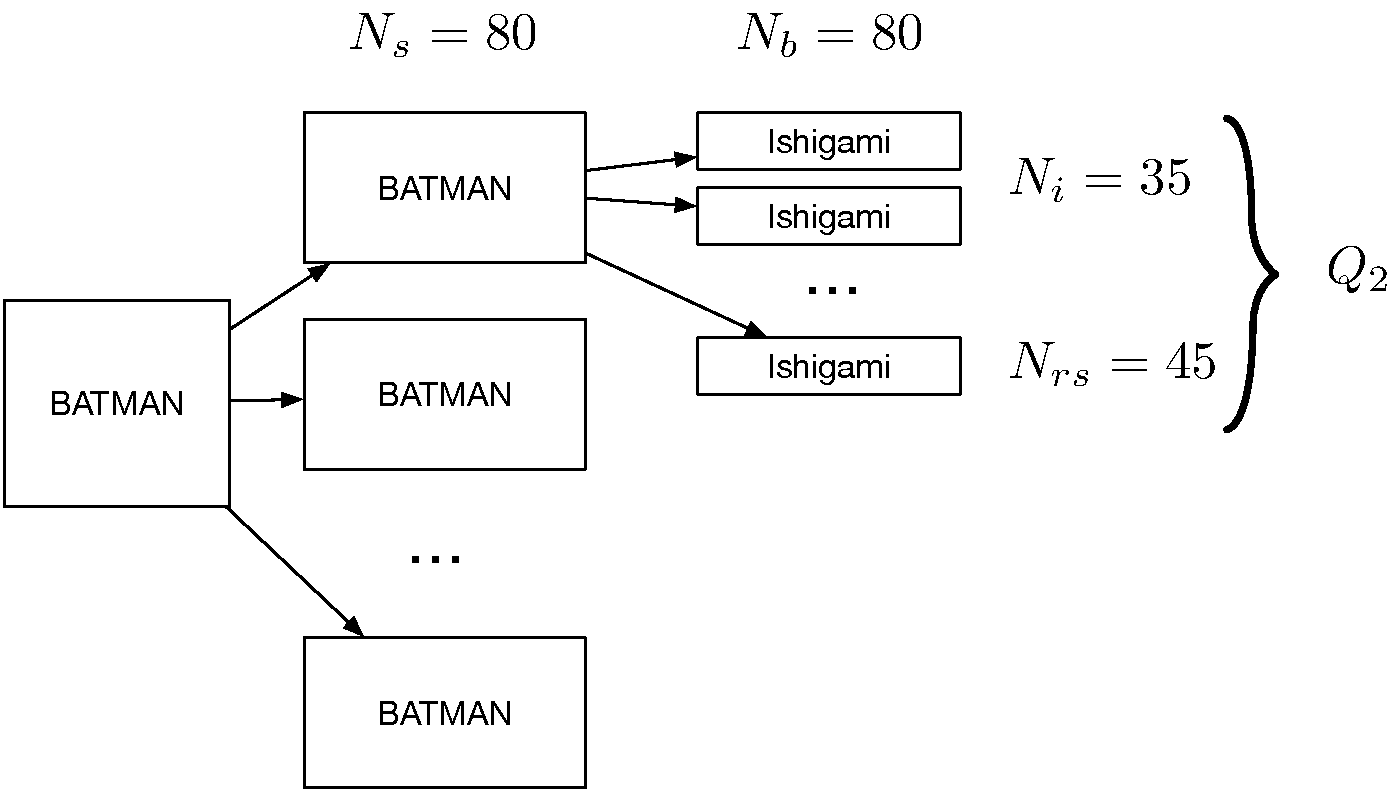
\includegraphics[width=0.8\linewidth,keepaspectratio]{fig/contributions/resample/4_1column_color-online-only_jpod-delta.pdf}
\caption{Example showing a computation of $Q_2$ with $N_i = 35, N_{rs} = 45$.}
\label{fig:jpod-delta}
\end{figure}

As shown in~\cref{fig:outer-delta}, there is no benefit of adding points outside the domain. Aside from the uniform distributions usually employed on this function, a standard arcsine distribution was also tested to assess the quality around boundaries but no enhancement was observed. When the delta space is increased, there is a loss of quality due to the presence of points in non-interesting regions.

\begin{figure*}[h]               
\centering
\subfloat[Uniform distribution]{
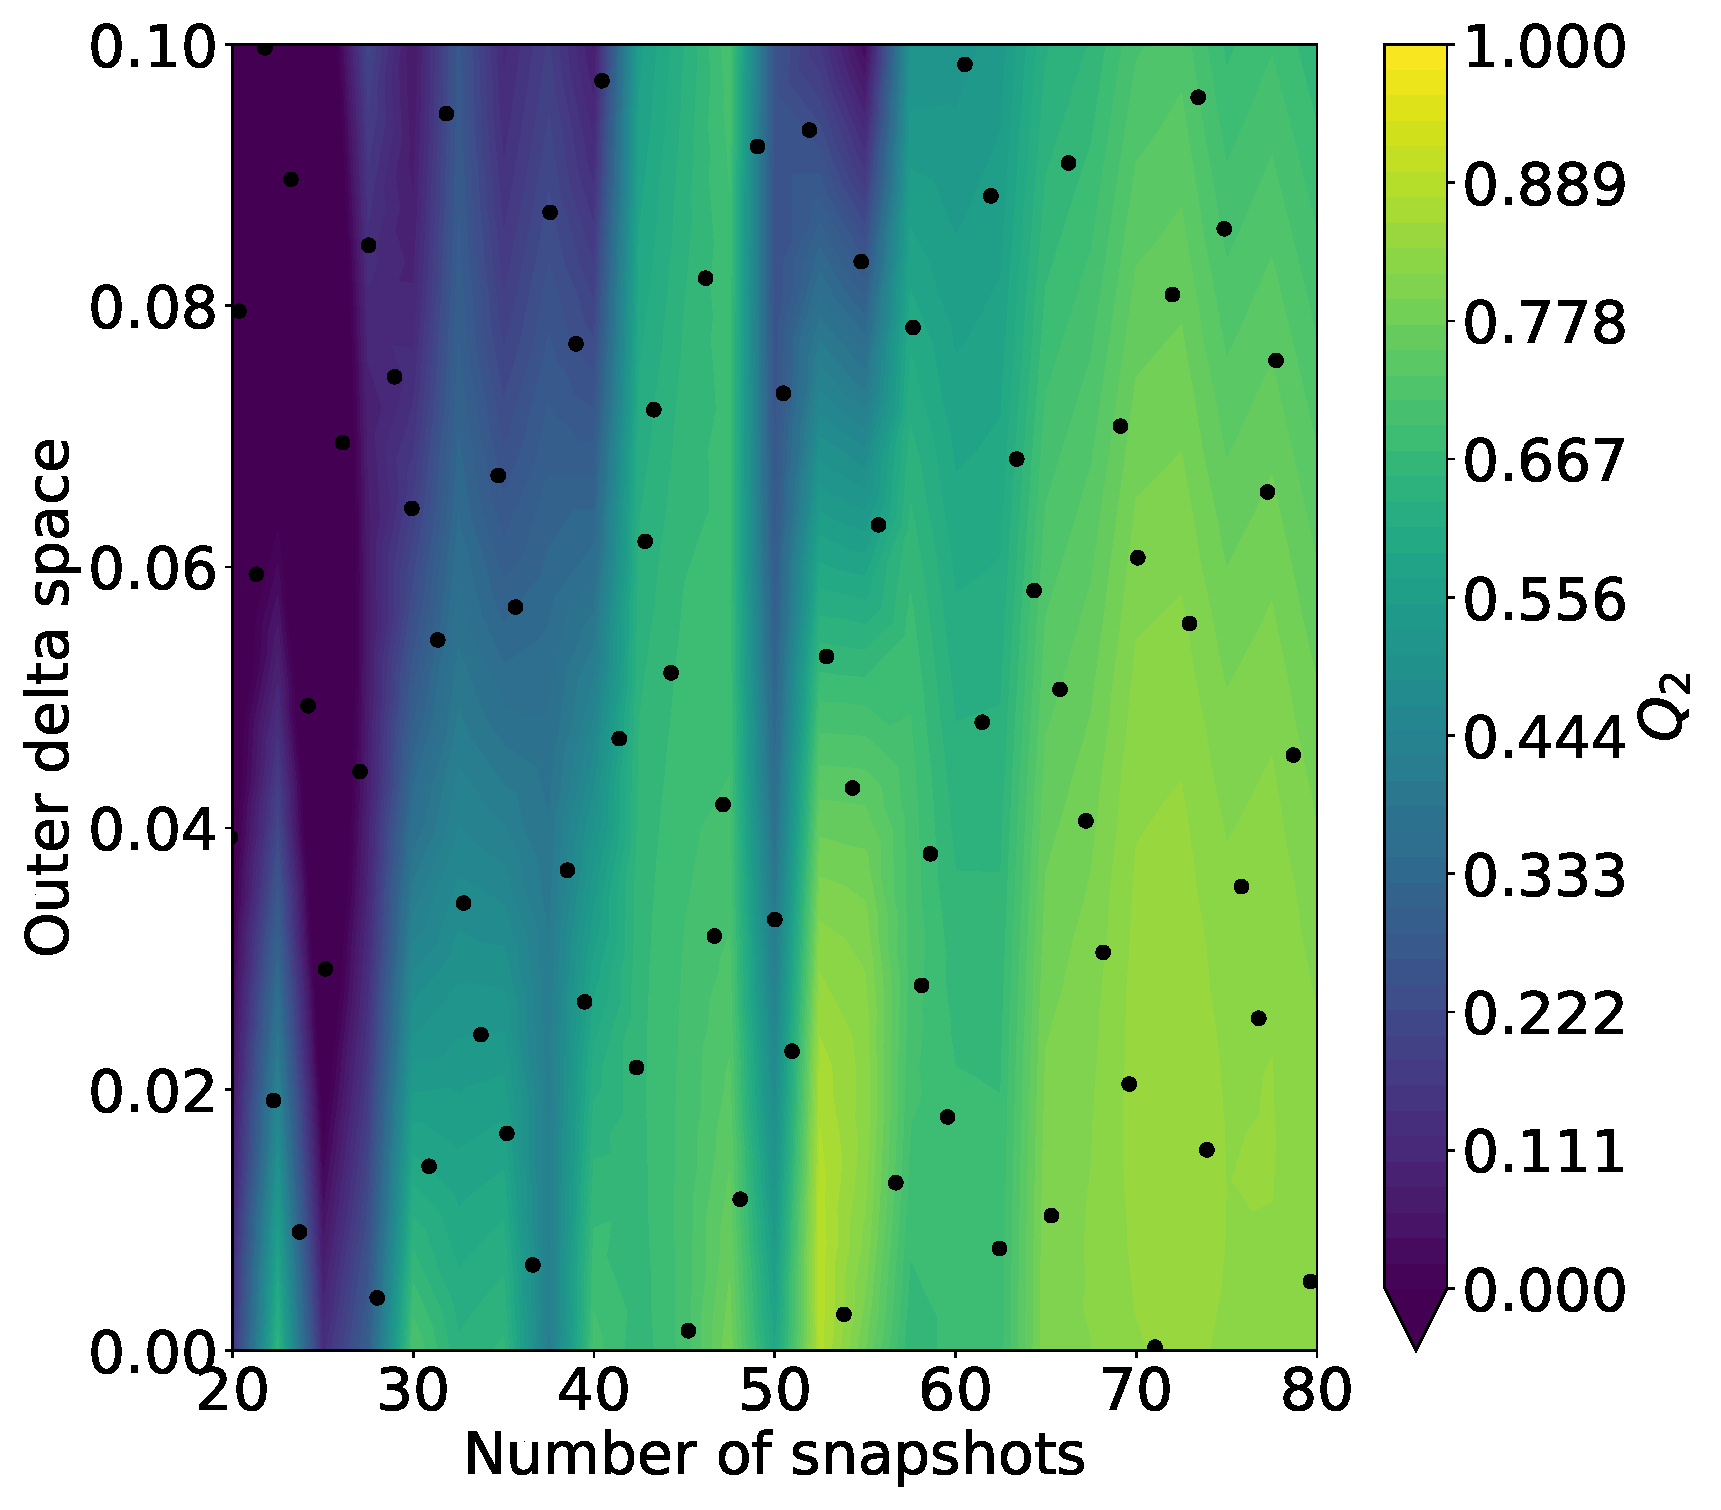
\includegraphics[width=0.47\linewidth,height=\textheight,keepaspectratio]{fig/contributions/resample/5a_2column_color-online-only_response_outer-delta_uniform.pdf}}
 ~       
\subfloat[Arcsine distribution]{
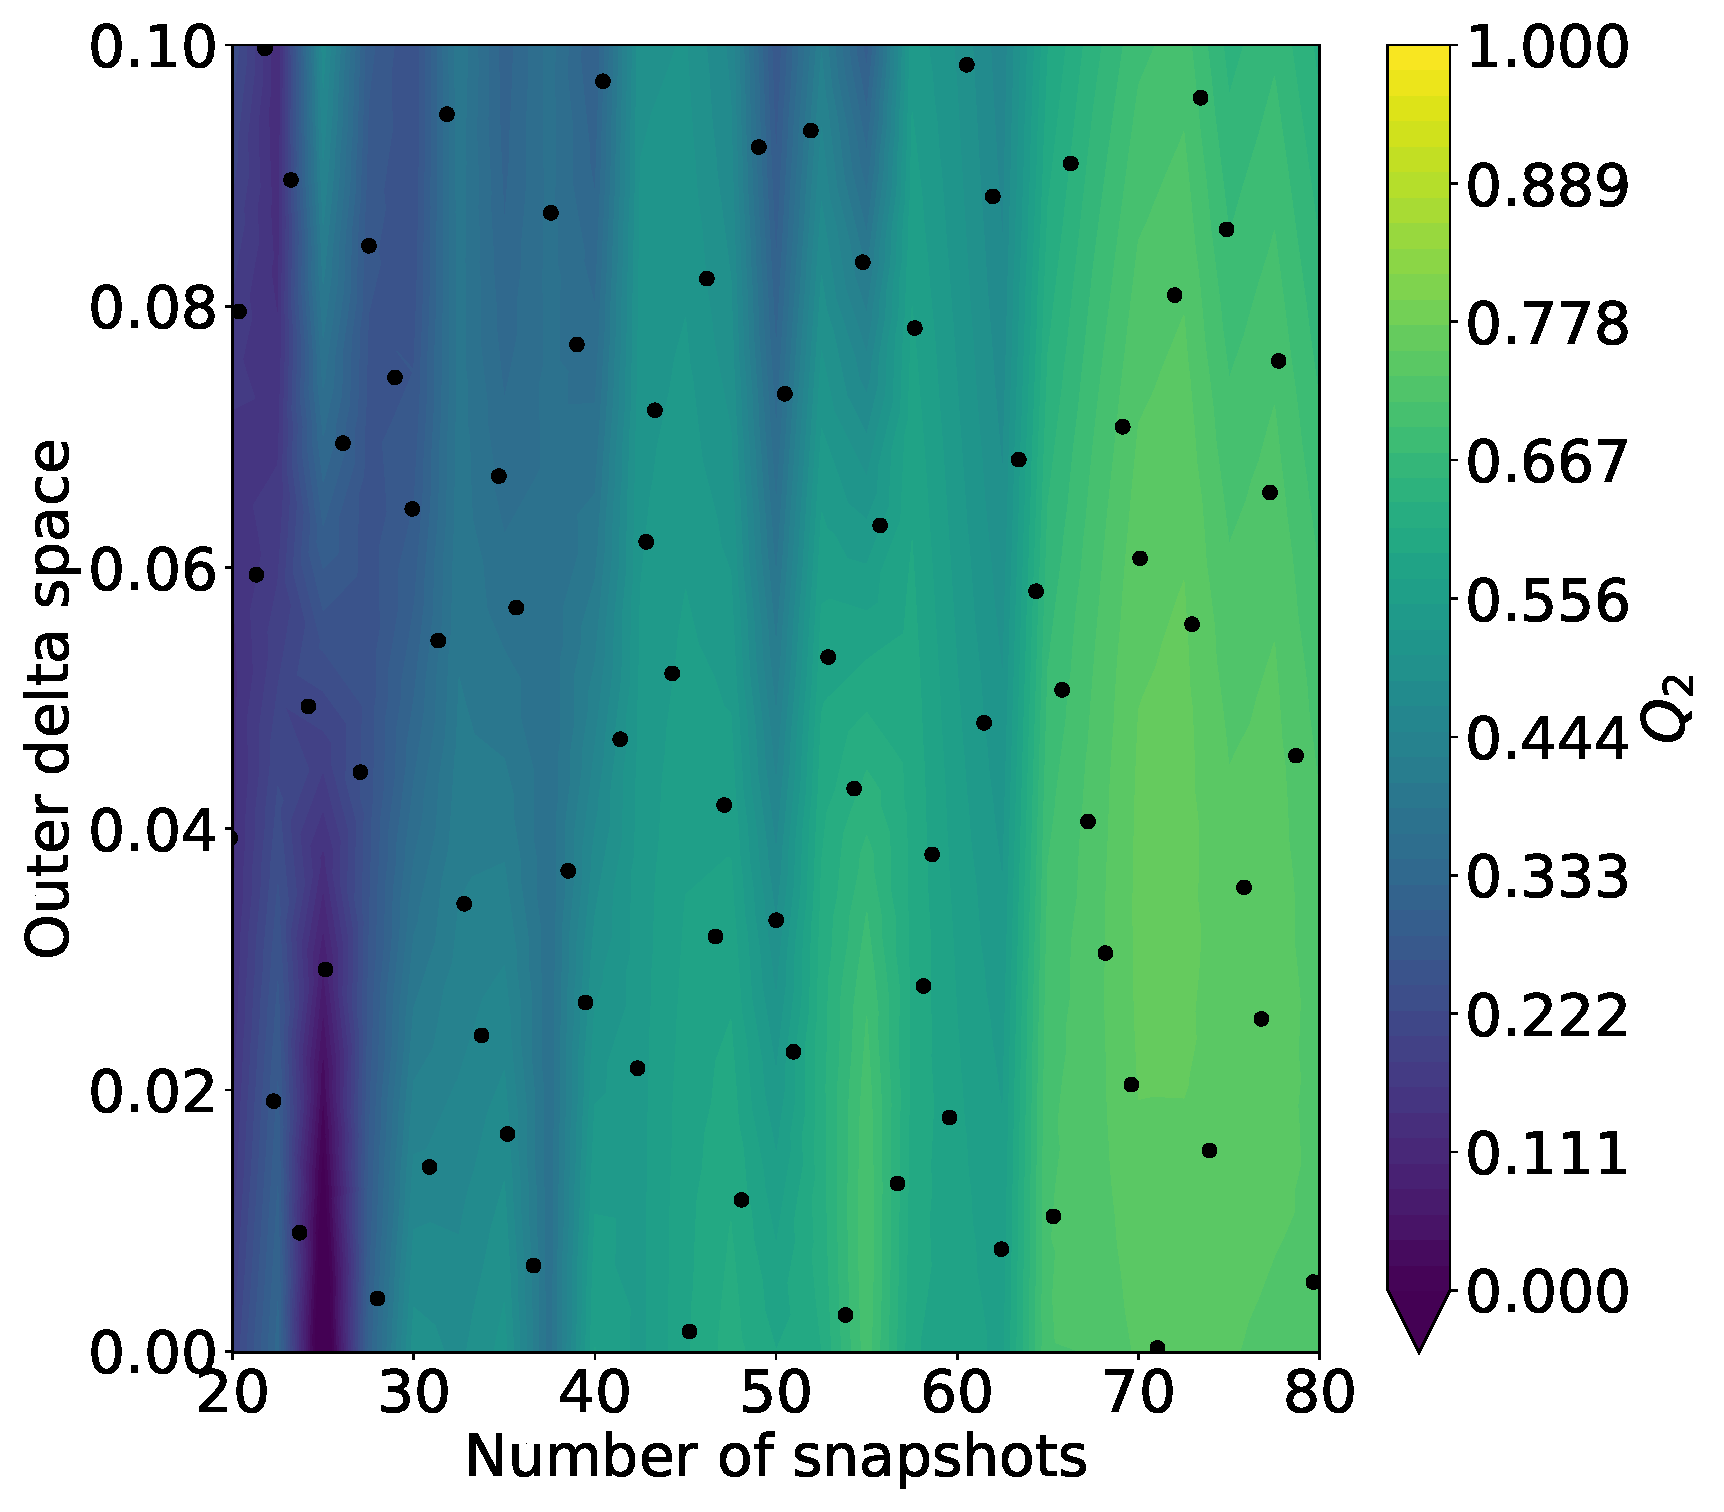
\includegraphics[width=0.47\linewidth,height=\textheight,keepaspectratio]{fig/contributions/resample/5b_2column_color-online-only_response_outer-delta_arcsine.pdf}}
\caption{Response surface of $Q_2$ function of the initial sample and the \textit{outer delta space}. Dots represent the simulations.}
\label{fig:outer-delta}
\end{figure*}

\begin{figure*}[h]               
\centering
\subfloat[Uniform distribution]{
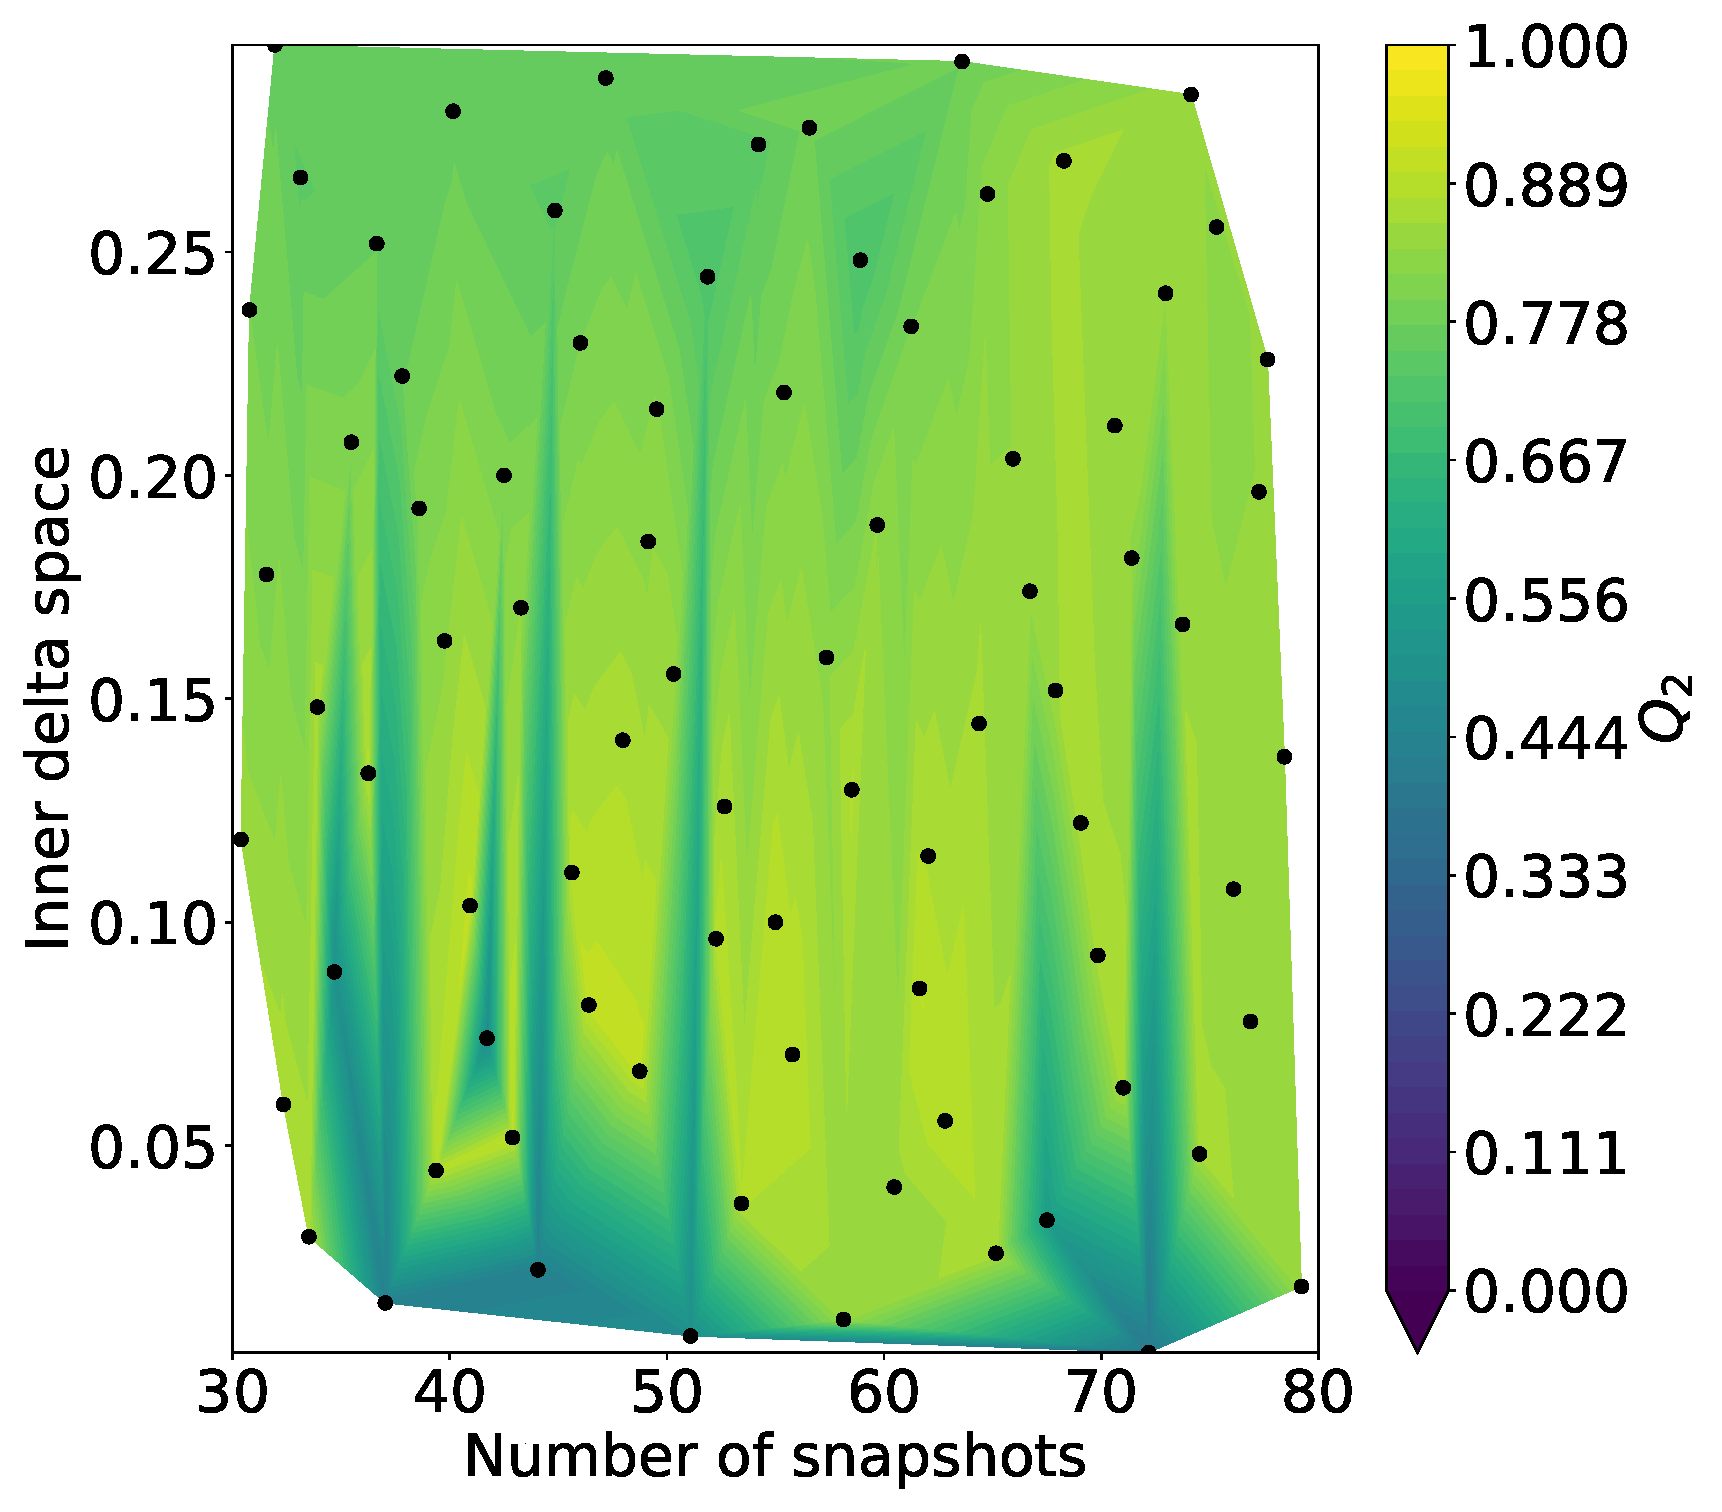
\includegraphics[width=0.47\linewidth,height=\textheight,keepaspectratio]{fig/contributions/resample/6a_2column_color-online-only_response_inner-delta_uniform.pdf}}
 ~       
\subfloat[Arcsine distribution]{
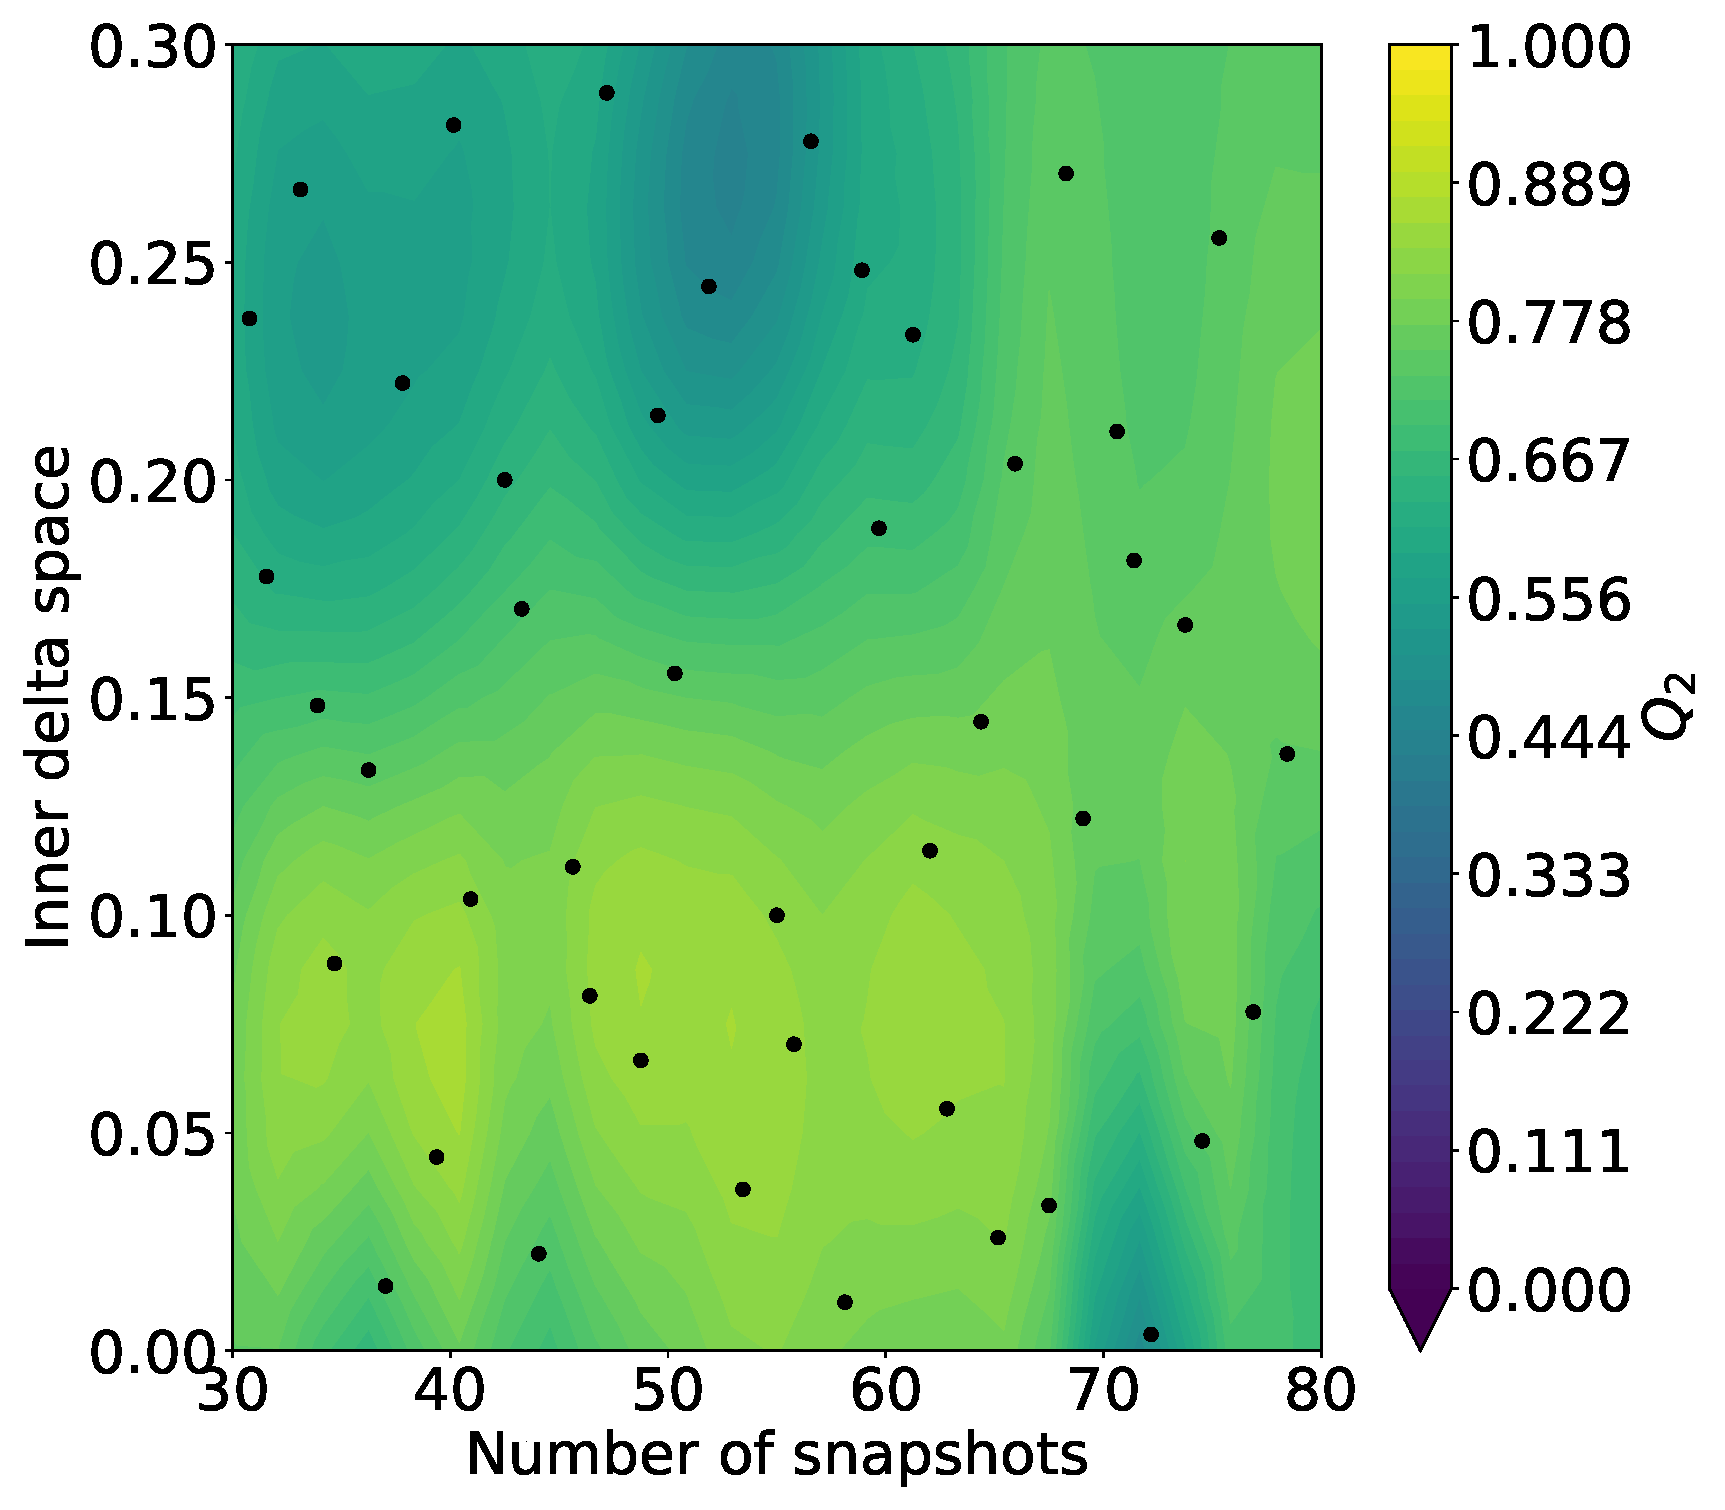
\includegraphics[width=0.47\linewidth,height=\textheight,keepaspectratio]{fig/contributions/resample/6b_2column_color-online-only_response_inner-delta_arcsine.pdf}}
\caption{Response surface of $Q_2$ function of the initial sample and the \textit{inner delta space}. Dots represent the simulations.}
\label{fig:inner-delta}
\end{figure*}

Complementary to this analysis using an outer delta space, an inner delta space factor has also been considered. The same methodology was used. Results are shown in \cref{fig:inner-delta}. On the uniform case, the model was not correctly computed due to high discontinuities caused by the ~0\% inner delta space cases. In~\cite{dette2010}, optimal design that tends to put more points near the boundaries was shown to be more effective. Our results are coherent with their findings as we observed an improvement of the quality when using a low inner delta space. Indeed, a small value of the parameter limits the trend to add points close to the boundaries.

This work has shown that setting an inner delta space comprised between 5 and 10\% is required to ensure the robustness of the model construction. Based on this observation, in the following the inner delta space is set to an arbitrary value of 8\%.

\subsection{Application on analytical functions}
\label{sec:res-functions}

The operating mechanism and catches of the methods can be visualized on the \textit{Rosenbrock} function---see~\cref{fig:methods-rosenbrock}. Starting from the $\sigma$ method: points are first added close to the top boundary despite the inner delta space parameter. However, the lack of surrounding points made this choice fairly legitimate. Other points seem to be located in interesting regions---where there is a gradient and no points. It can be seen as a low discrepancy sequence, which made its use relevant for studying the delta space impact in \cref{sec:delta-space}. On the other hand, the LOO-$\sigma$ method does not seem to exhibit a boundary preference. But, on the bottom left-hand corner, there is an accumulation of points. Indeed, this method relies on the location of the most sensitive point. Considering the surroundings of a strong extremum---as it is the case here---, the method tends to add points first in this zone preventing further exploration of the domain and, in this case, totally misses the second extremum. Lastly, the LOO-\textit{Sobol'} method seems more balanced. Points have been added preferentially on the $X_1$ parameter axis, as it is slightly the most influent parameter ($S_{T_{X_1}} \simeq 0.7$). 

\begin{figure*}[!h]               
\centering
\subfloat[$\sigma$: $Q_2 = 0.75$]{
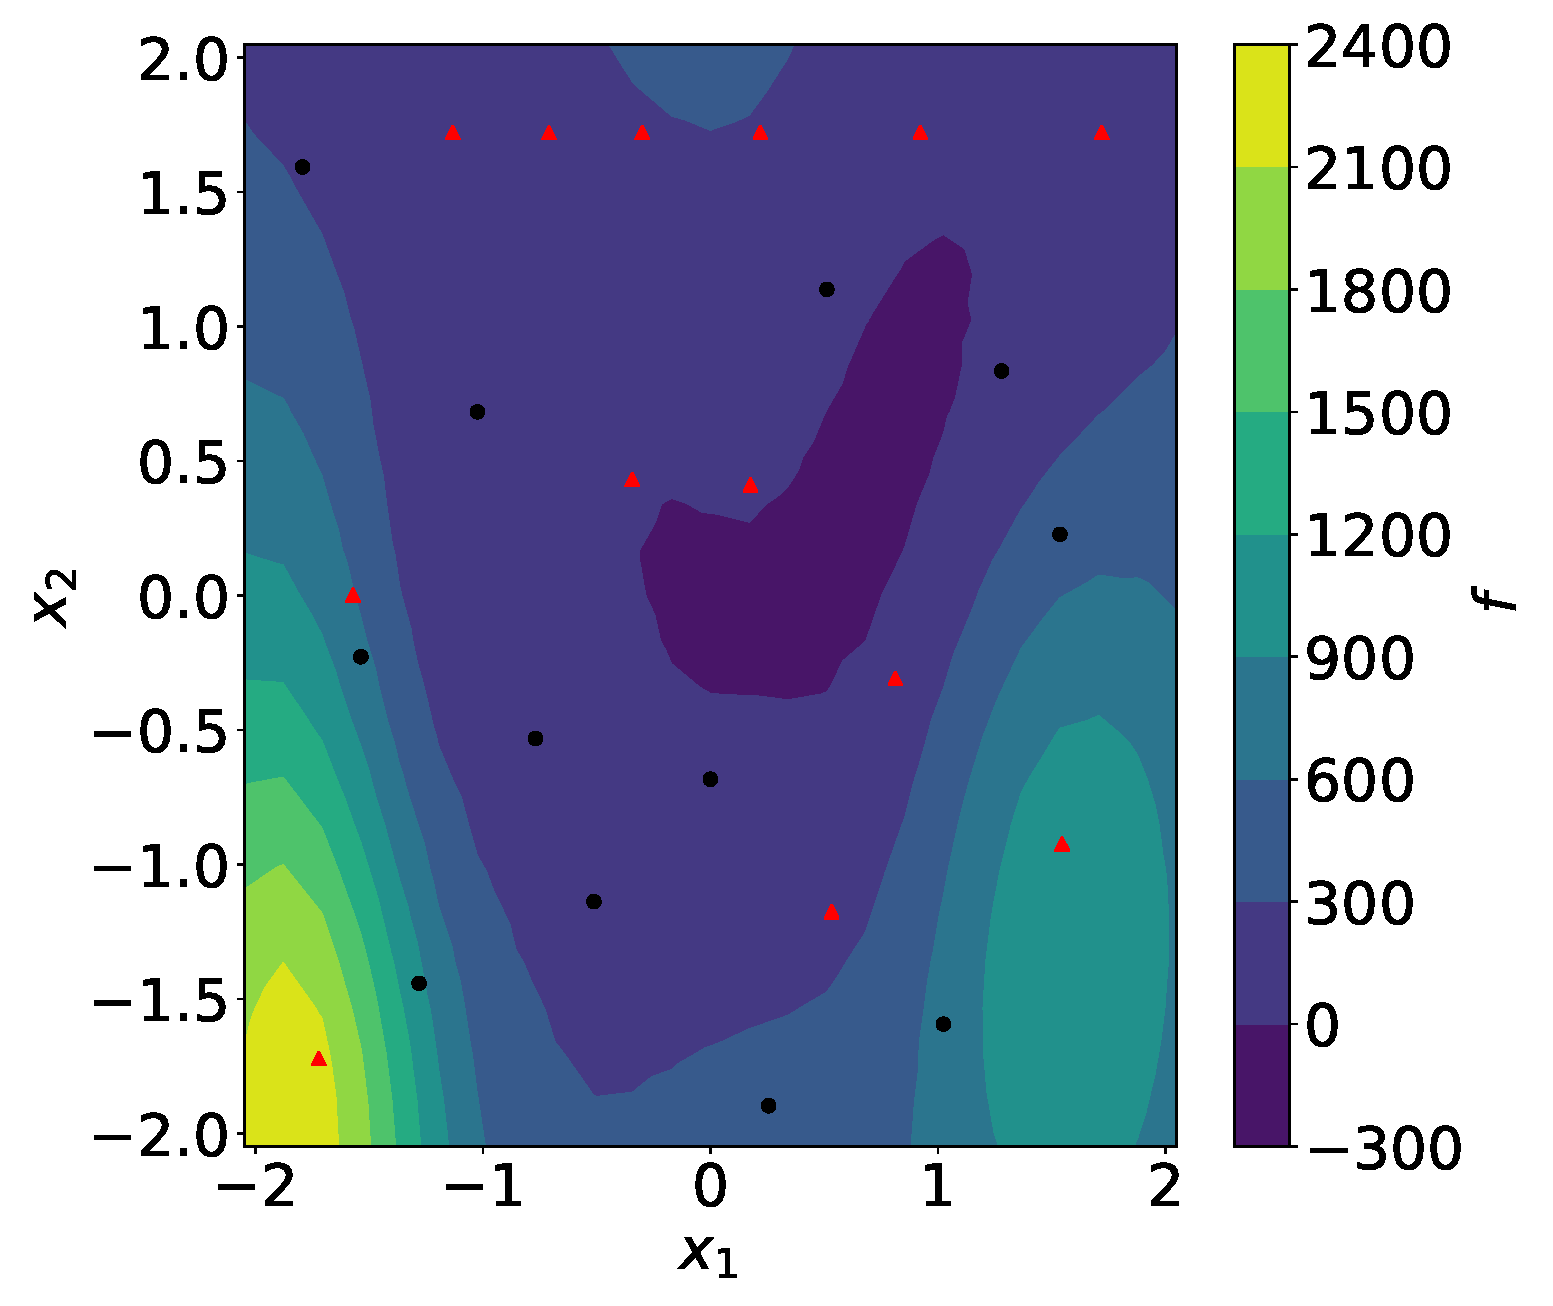
\includegraphics[width=0.47\linewidth,height=\textheight,keepaspectratio]{fig/contributions/resample/7a_2column_color-online-only_response_rosen_Ns12_sigma.pdf}}
 ~       
\subfloat[LOO-$\sigma$: $Q_2 = 0.68$]{
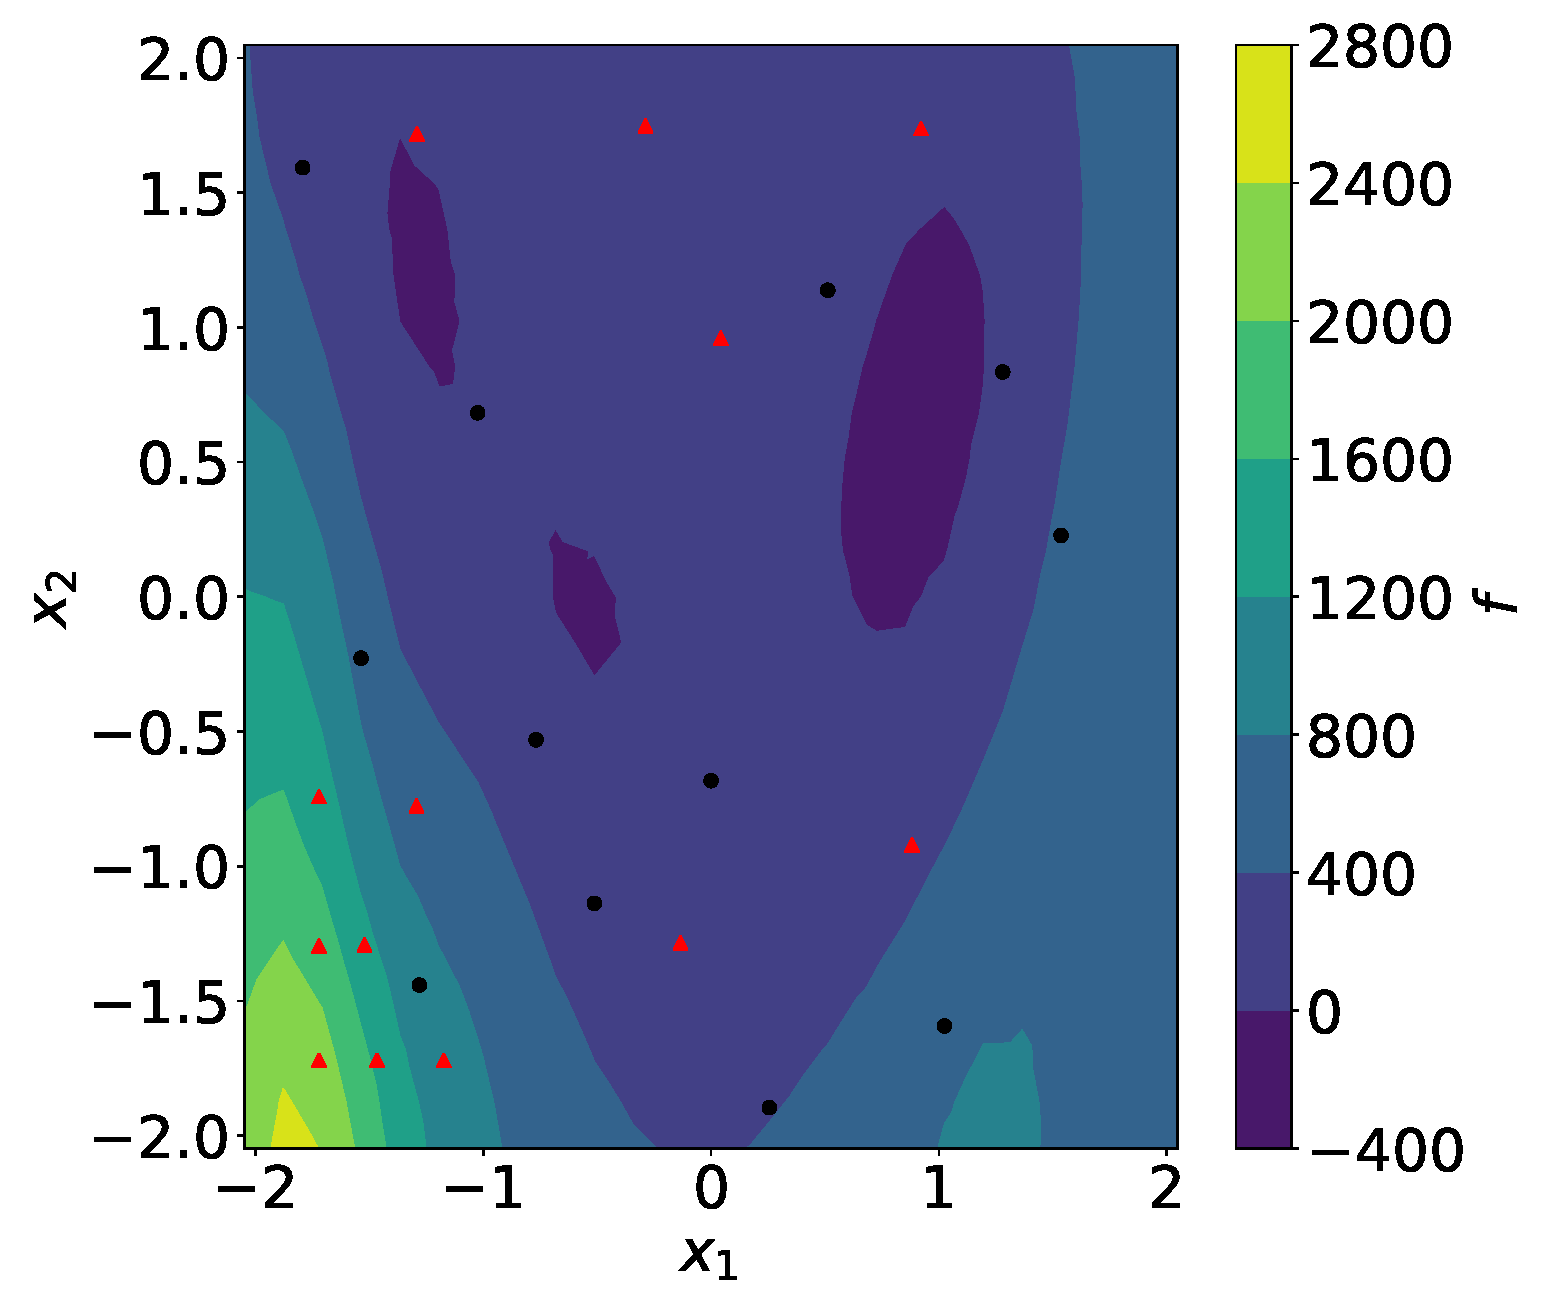
\includegraphics[width=0.47\linewidth,height=\textheight,keepaspectratio]{fig/contributions/resample/7b_2column_color-online-only_response_rosen_Ns12_loo-sigma.pdf}}
      
\subfloat[LOO-\textit{Sobol'}: $Q_2 = 0.86$]{
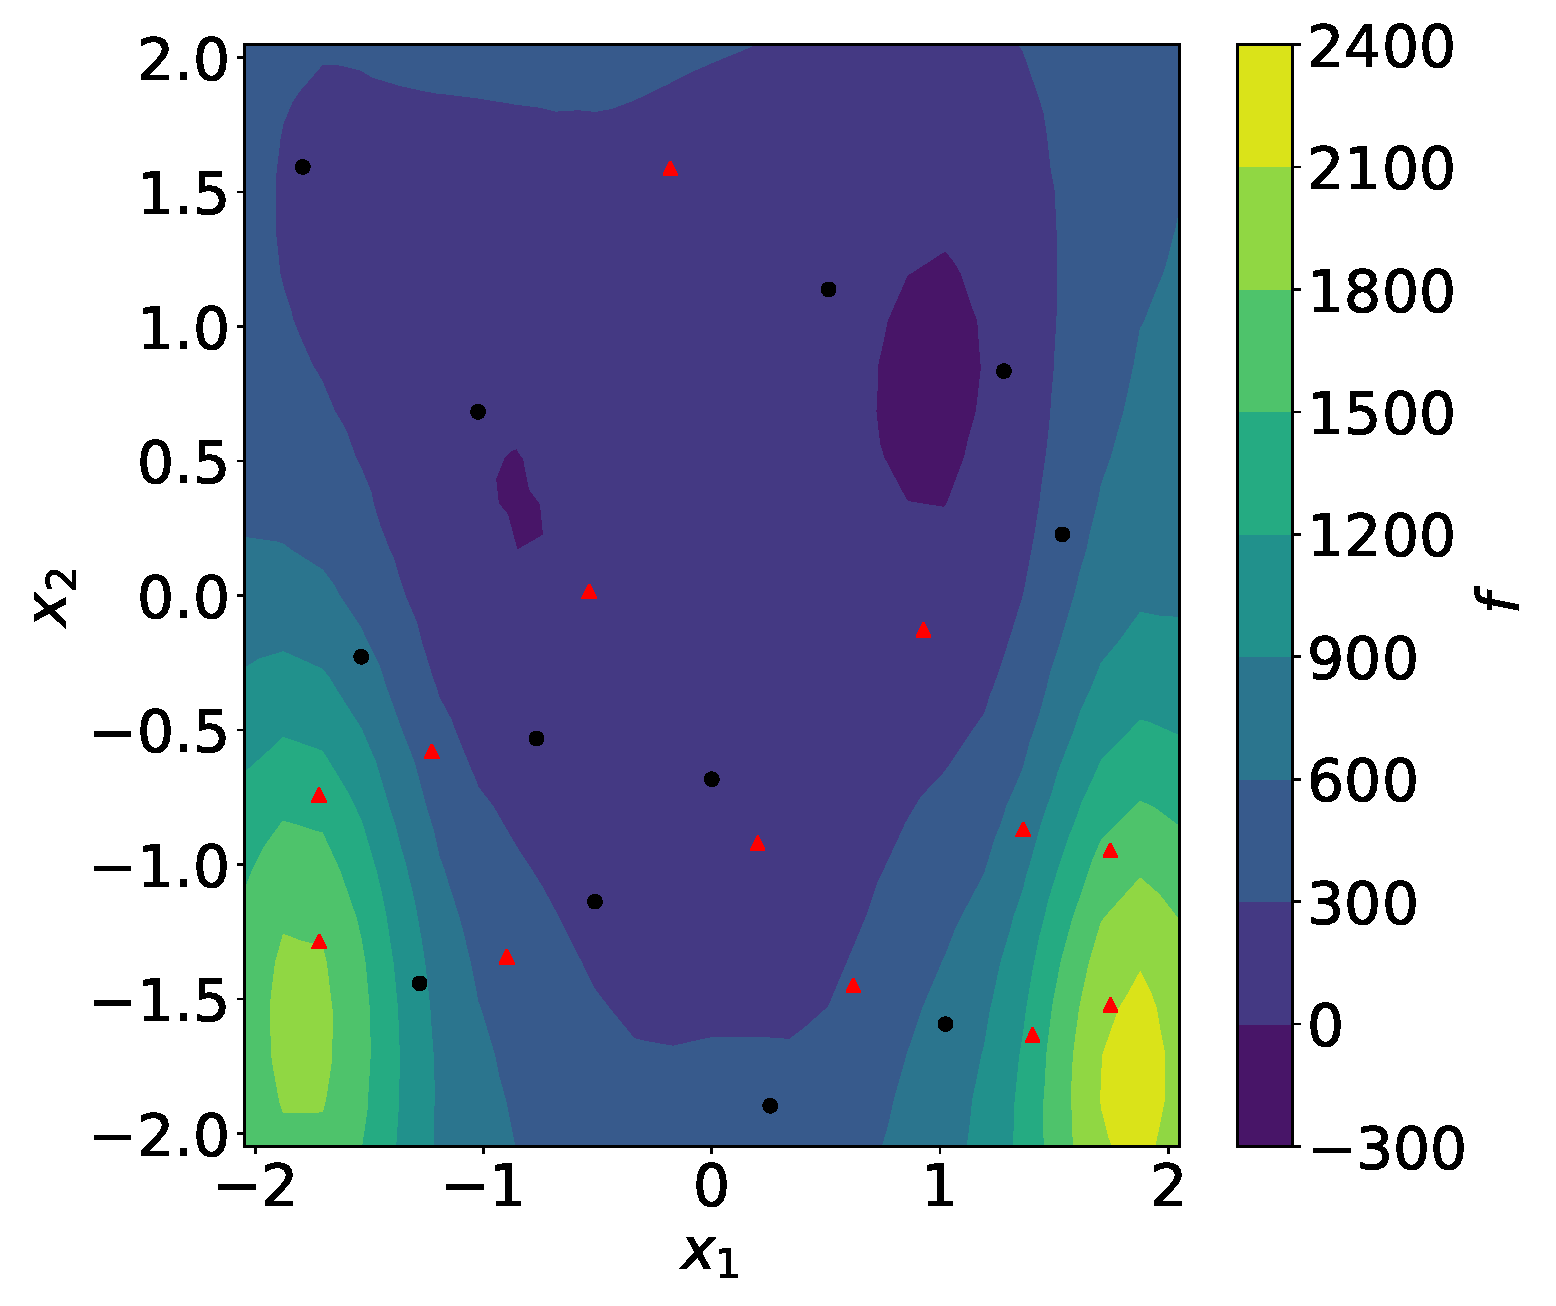
\includegraphics[width=0.47\linewidth,height=\textheight,keepaspectratio]{fig/contributions/resample/7c_2column_color-online-only_response_rosen_Ns12_loo-sobol.pdf}}
\caption{Response surface of the \textit{Rosenbrock} function. In each case, the initial learning sample is composed of 12 simulations and there are 13 resampling points---respectively represented in dots and diamonds.}
\label{fig:methods-rosenbrock}
\end{figure*}

A convergence study has also been performed. With a fixed total number of simulations, the size of the initial learning sample was changed to evaluate the impact of the ratio of the initial sampling over the total number of samples on the quality of the model. As in~\cref{sec:delta-space}, a \textit{Halton} sequence was used. The respective parameters are reported in~\cref{tab:cv-budget-q2}. The \textit{Sobol'} indices: for the \textit{Ishigami} function are found in~\cite{marrel2012}; for the \textit{g-function} function are found in~\cite{kucherenko2016}; while for the \textit{Rosenbrock} function, a stochastic sample of $\numprint{100000}$ evaluations was used.

\begin{table*}
\centering
\begin{tabular}{lccl}
\toprule
Function &Sample Budget & $Q_2$ & Total order \textit{Sobol'} indices \\
\cmidrule{1-3}
\textit{Rosenbrock} 2-D & 25 & 0.82 & [0.71, 0.50]\\
\textit{Ishigami} 3-D & 80 & 0.85 & [0.557, 0.443, 0.244]\\
\textit{g-function} 4-D & 65 & 0.66& [0.60,  0.27,  0.15,  0.10]\\
\textit{g-function} 11-D (i)& 80 & 0.84& [0.69, 0.31, 0, ..., 0]\\
\textit{g-function} 11-D (ii)& 80 & 0.66 & [0.47, 0.21, 0.21, 0.12, 0.12, 0.02, 0, ..., 0]\\
\bottomrule
\end{tabular}
\caption{Reference $Q_2$ and Total order \textit{Sobol'} indices. Theoretical values for both \emph{Ishigami} and \emph{g-function} and computed for \emph{Rosenbrock}.}
\label{tab:cv-budget-q2}
\end{table*}

\begin{figure*}[!h]
\centering
\subfloat[\textit{Rosenbrock}]{
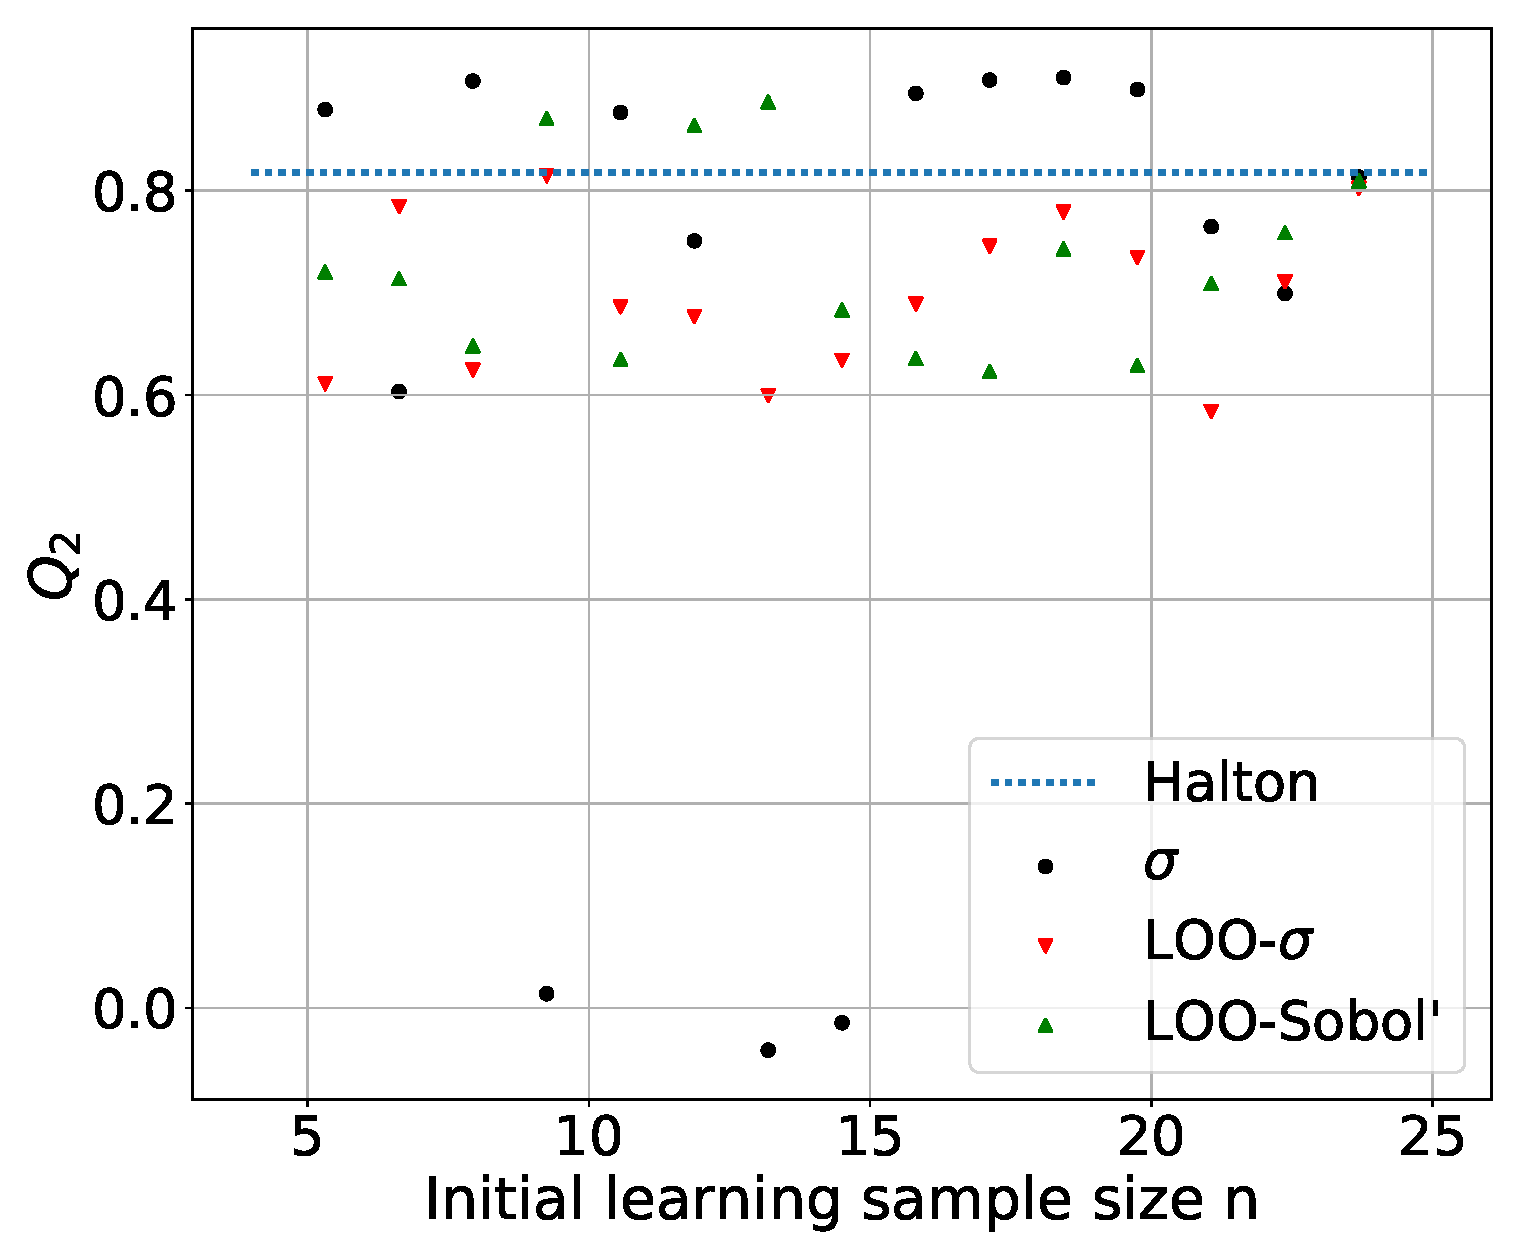
\includegraphics[width=0.47\linewidth,height=\textheight,keepaspectratio]{fig/contributions/resample/8a_2column_color-online-only_conv_q2_Rosenbrock.pdf}}
 ~       
\subfloat[\textit{Ishigami}]{
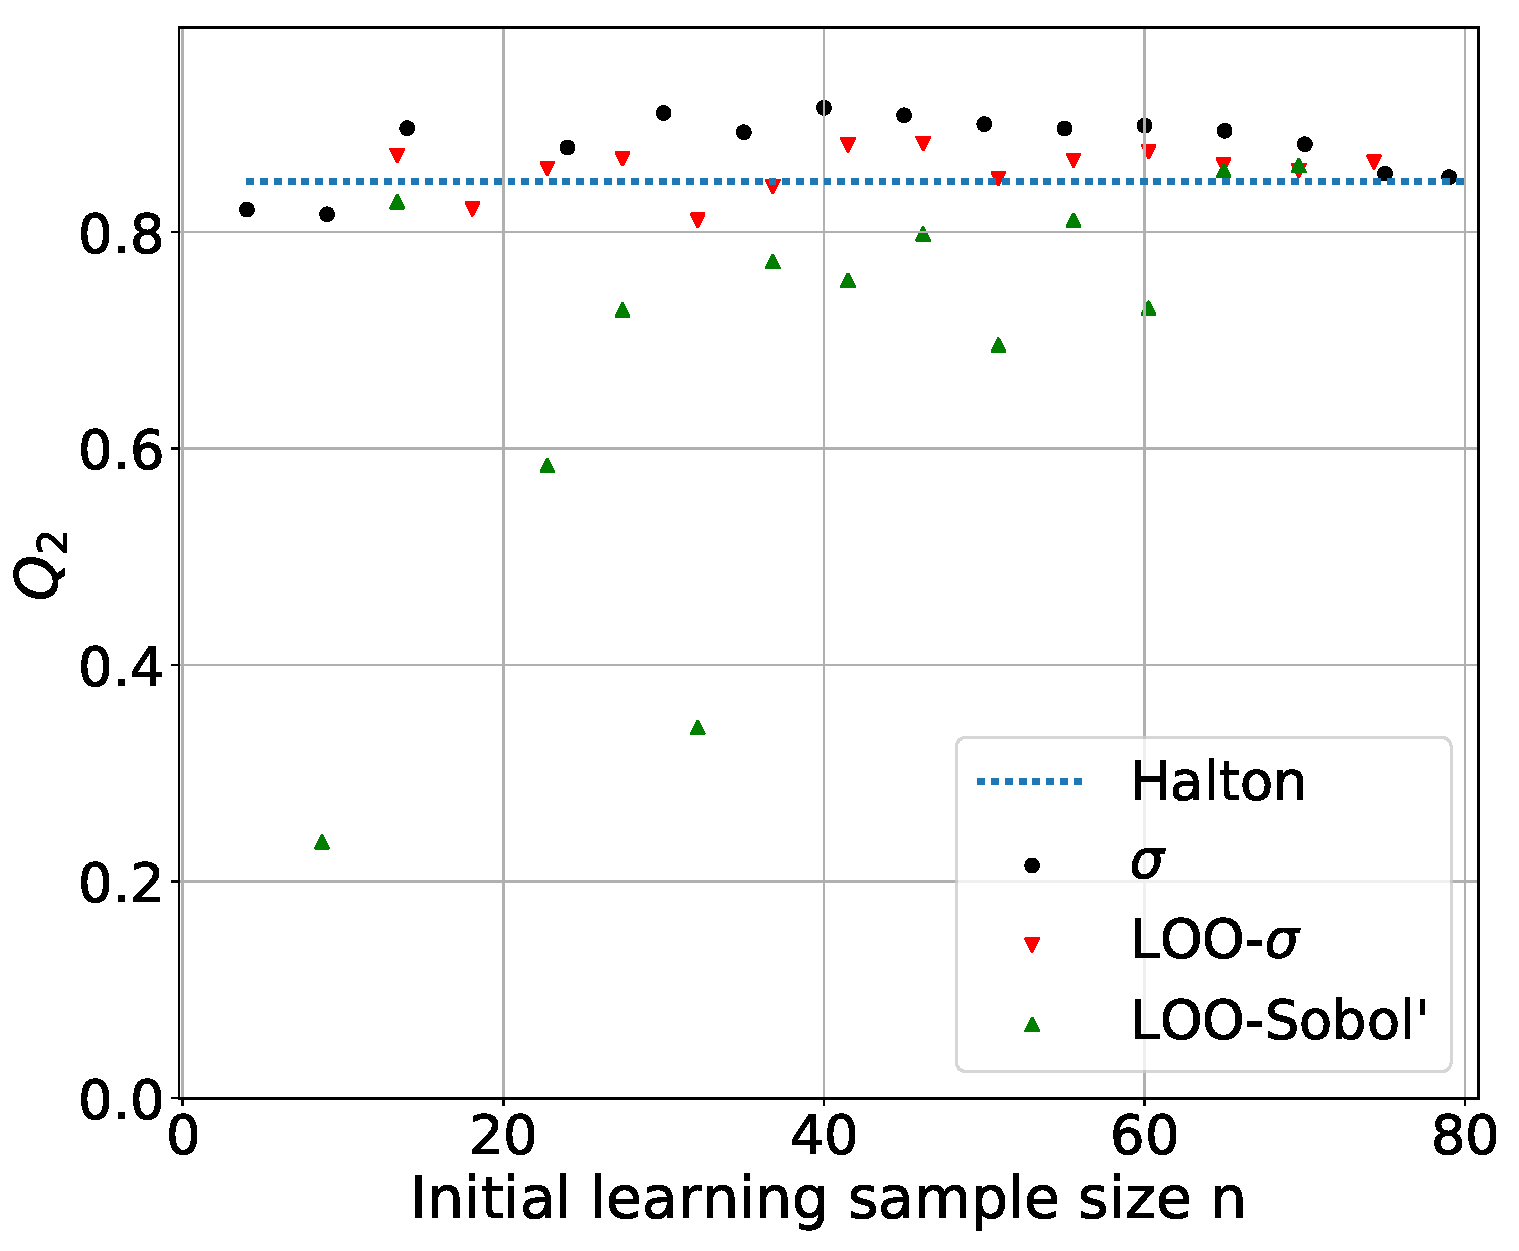
\includegraphics[width=0.47\linewidth,height=\textheight,keepaspectratio]{fig/contributions/resample/8b_2column_color-online-only_conv_q2_Ishigami.pdf}}
        
\subfloat[\textit{4-D g-function}]{
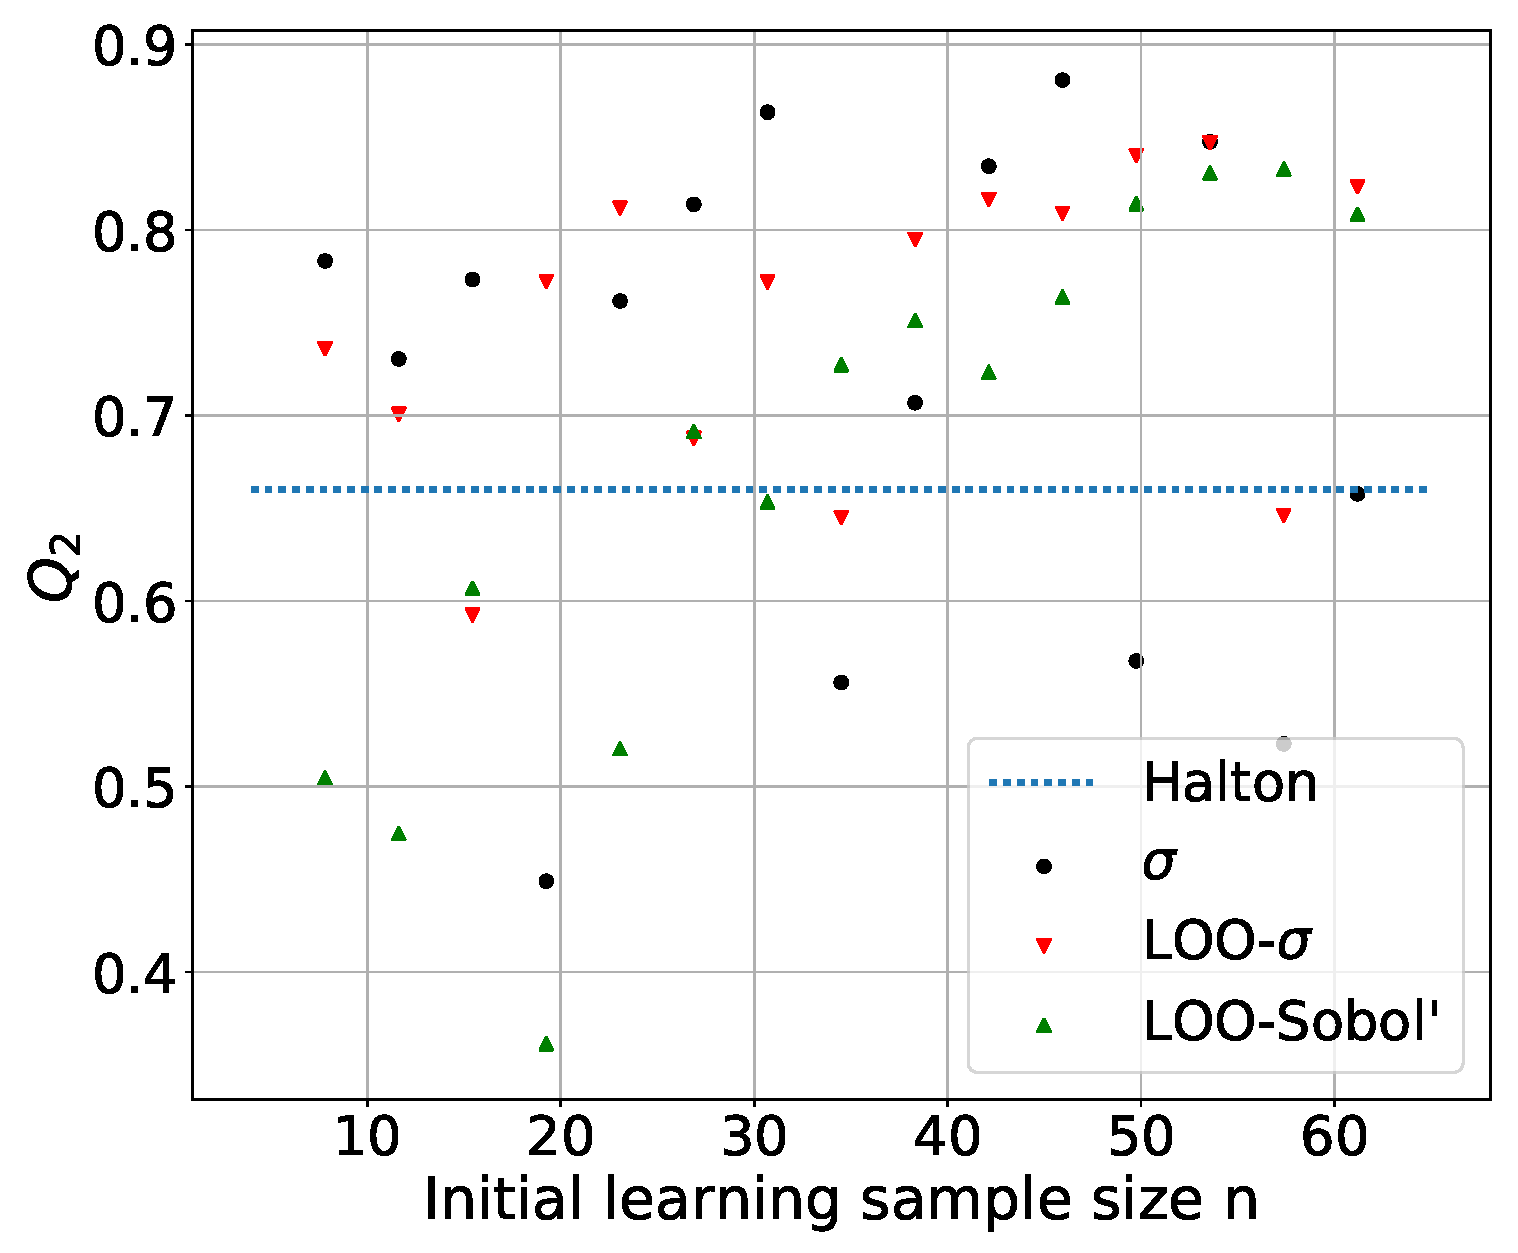
\includegraphics[width=0.46\linewidth,height=\textheight,keepaspectratio]{fig/contributions/resample/8c_2column_color-online-only_conv_q2_Gfunction.pdf}}

\subfloat[\textit{11-D g-function (i)}]{
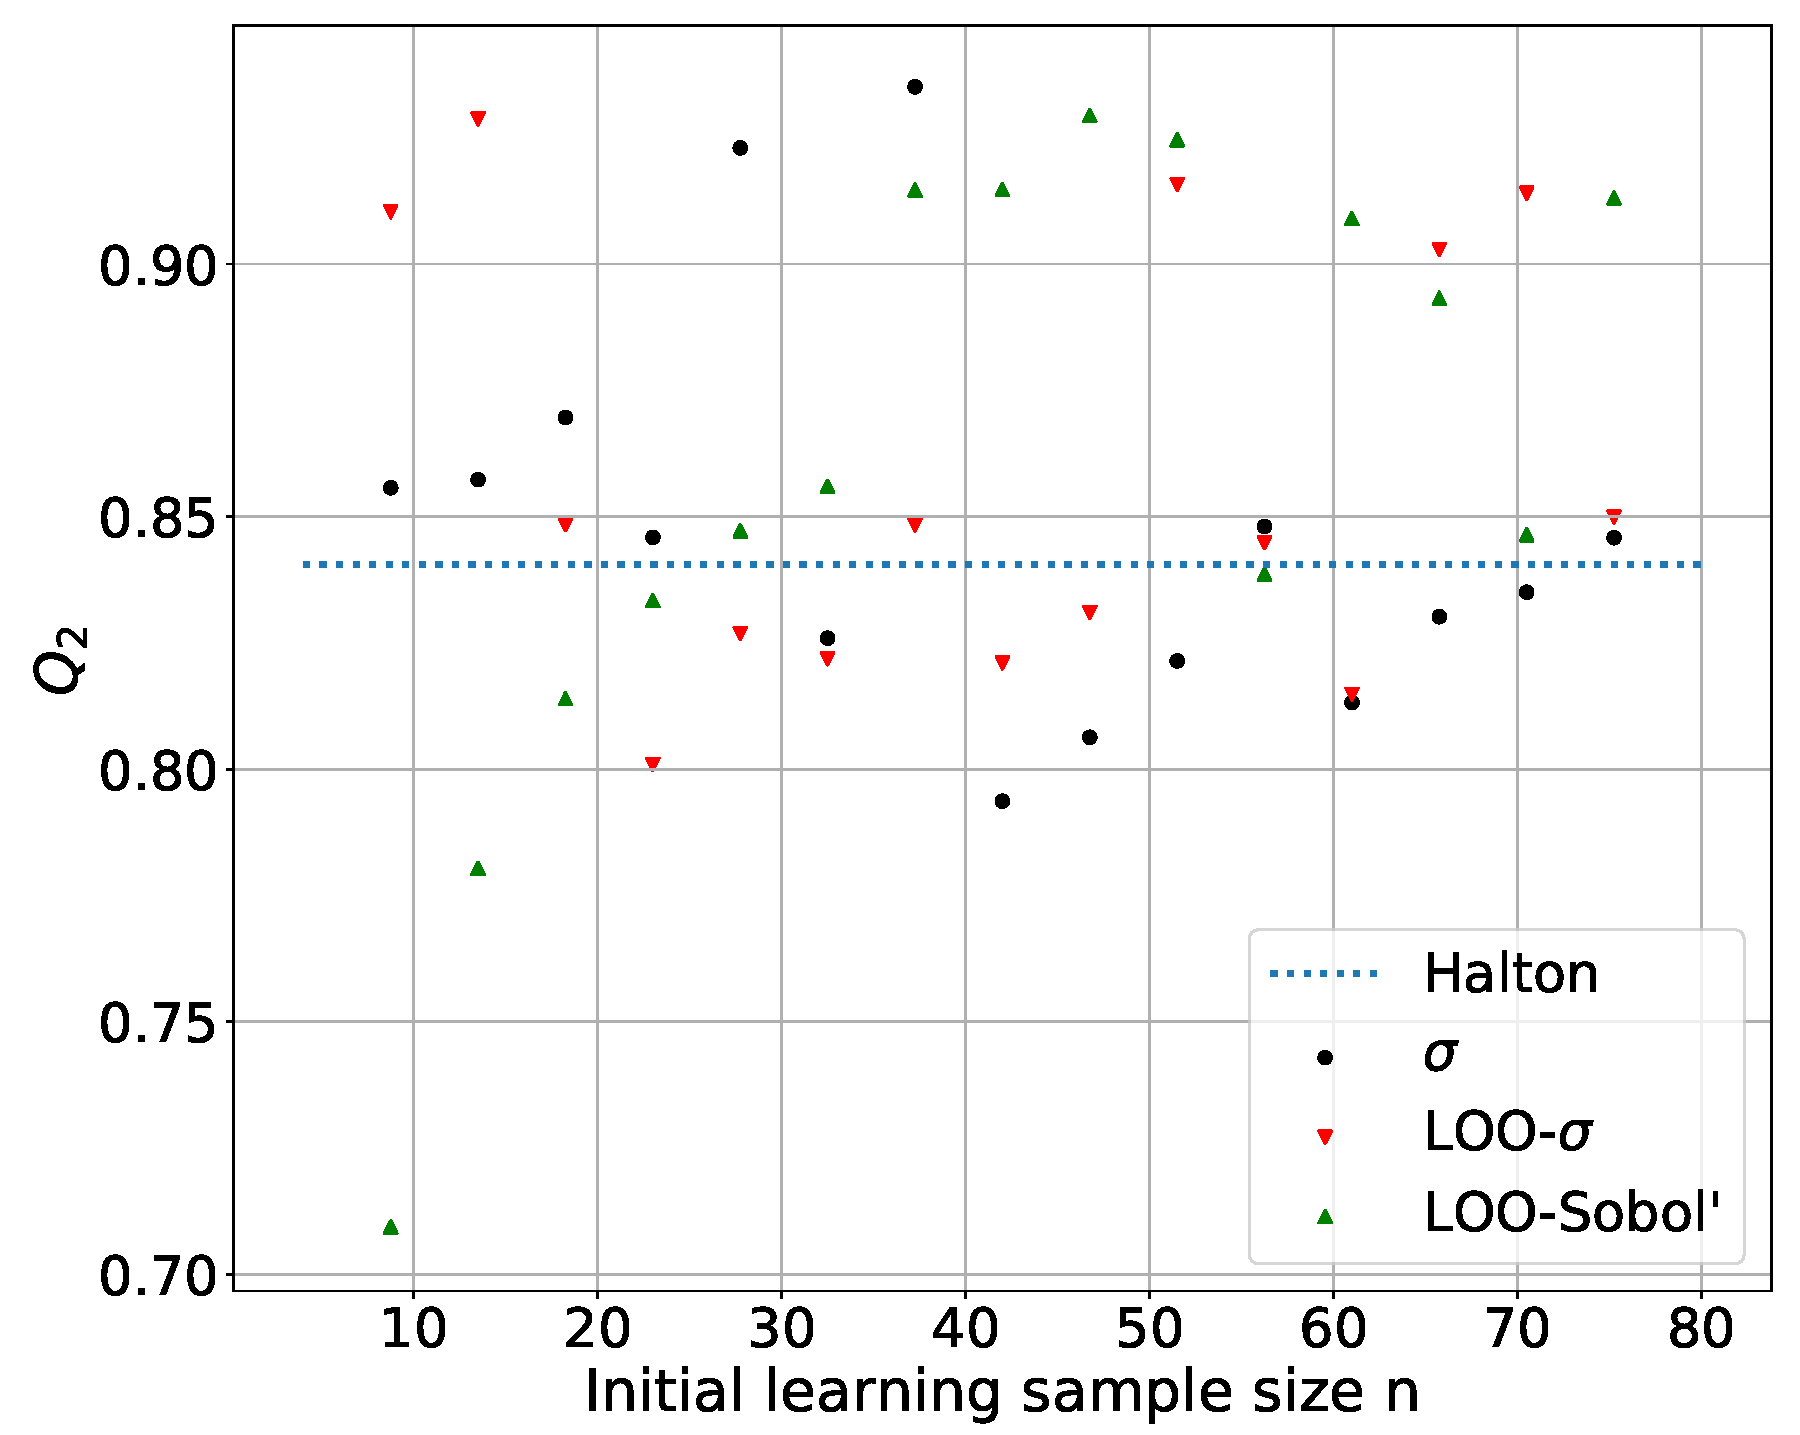
\includegraphics[width=0.47\linewidth,height=\textheight,keepaspectratio]{fig/contributions/resample/8d_2column_color-online-only_conv_q2_Gfunction11.pdf}}
~
\subfloat[\textit{11-D g-function (ii)}]{
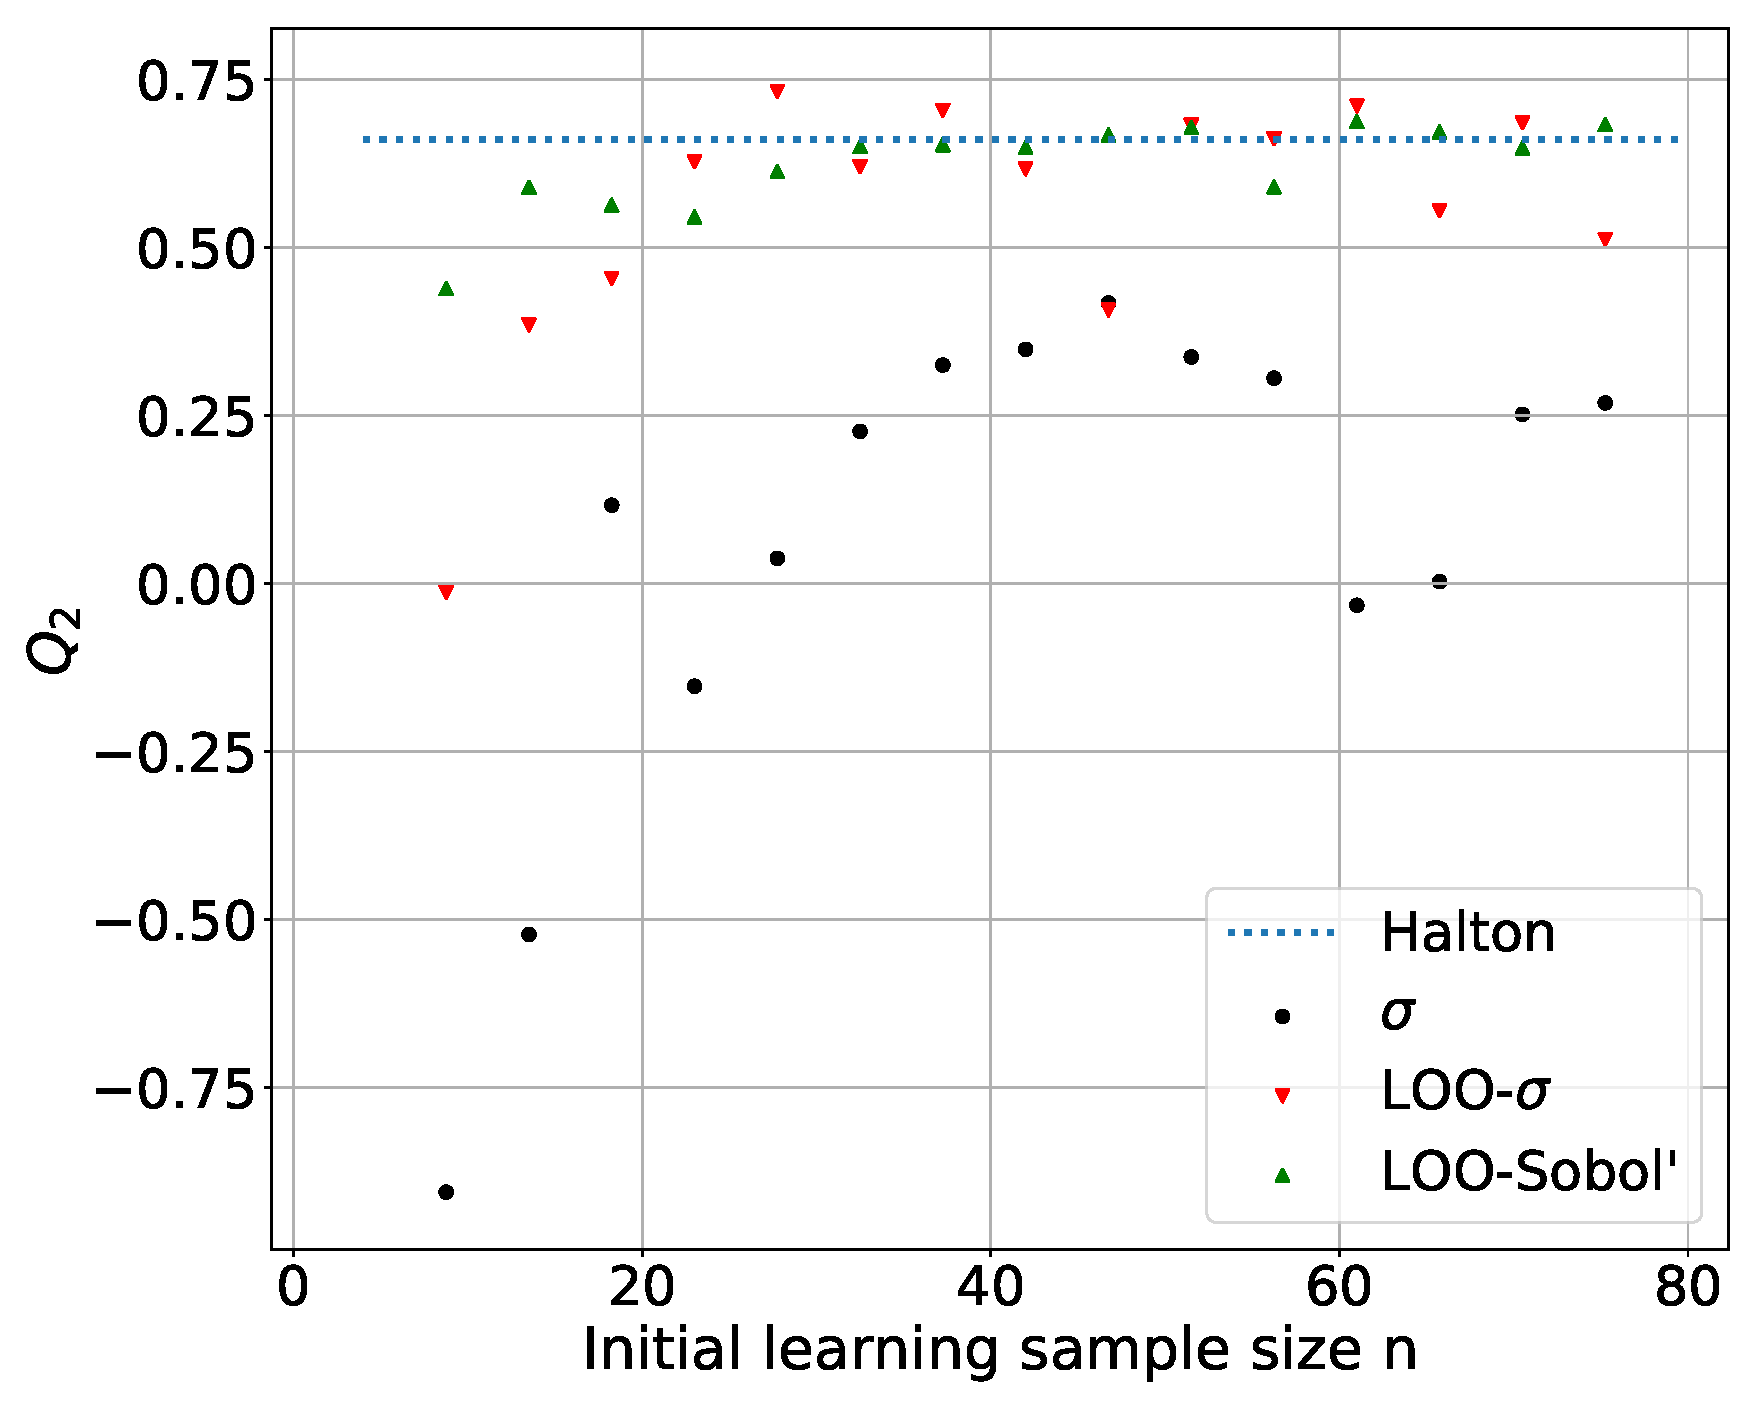
\includegraphics[width=0.47\linewidth,height=\textheight,keepaspectratio]{fig/contributions/resample/8e_2column_color-online-only_conv_q2_Gfunction11.pdf}}
\caption{Convergence of $Q_2$ of the different methods on each function by varying the initial learning sample size with a fixed budget.}
\label{fig:methods-cv}
\end{figure*}

Results are shown in~\cref{fig:methods-cv}. The $\sigma$ method appears to be one of the most, in some cases the most, effective method but it also exhibits more variability. Increasing dimensionality seems only to improve slightly this behaviour. There are multiple explanations to this phenomenon. The method relies on the use of an inference about the variance of the model. Starting from a given sample, if the fitting process does not converge, the prediction of the variance will be far from correct leading to a wrong resampling. Of course, there is a chance for this new point location to be relevant. This can lead to an even worse model or an overfitting where the model is too closely linked to the outputs, so the model has memorized only the feature but not learned the underlining correlation between the data. Lastly, looking at~\cref{fig:methods-rosenbrock-nofit}, even if the points look well distributed over the parameter space, the pGP model is absolutely wrong. The Gaussian Process reconstruction failed to recover the response surface of the function whereas a Radial Basis Function Networks model successfully did it.

\begin{figure*}[!h]               
\centering
\subfloat[Gaussian Process: $Q_2 = 0$]{
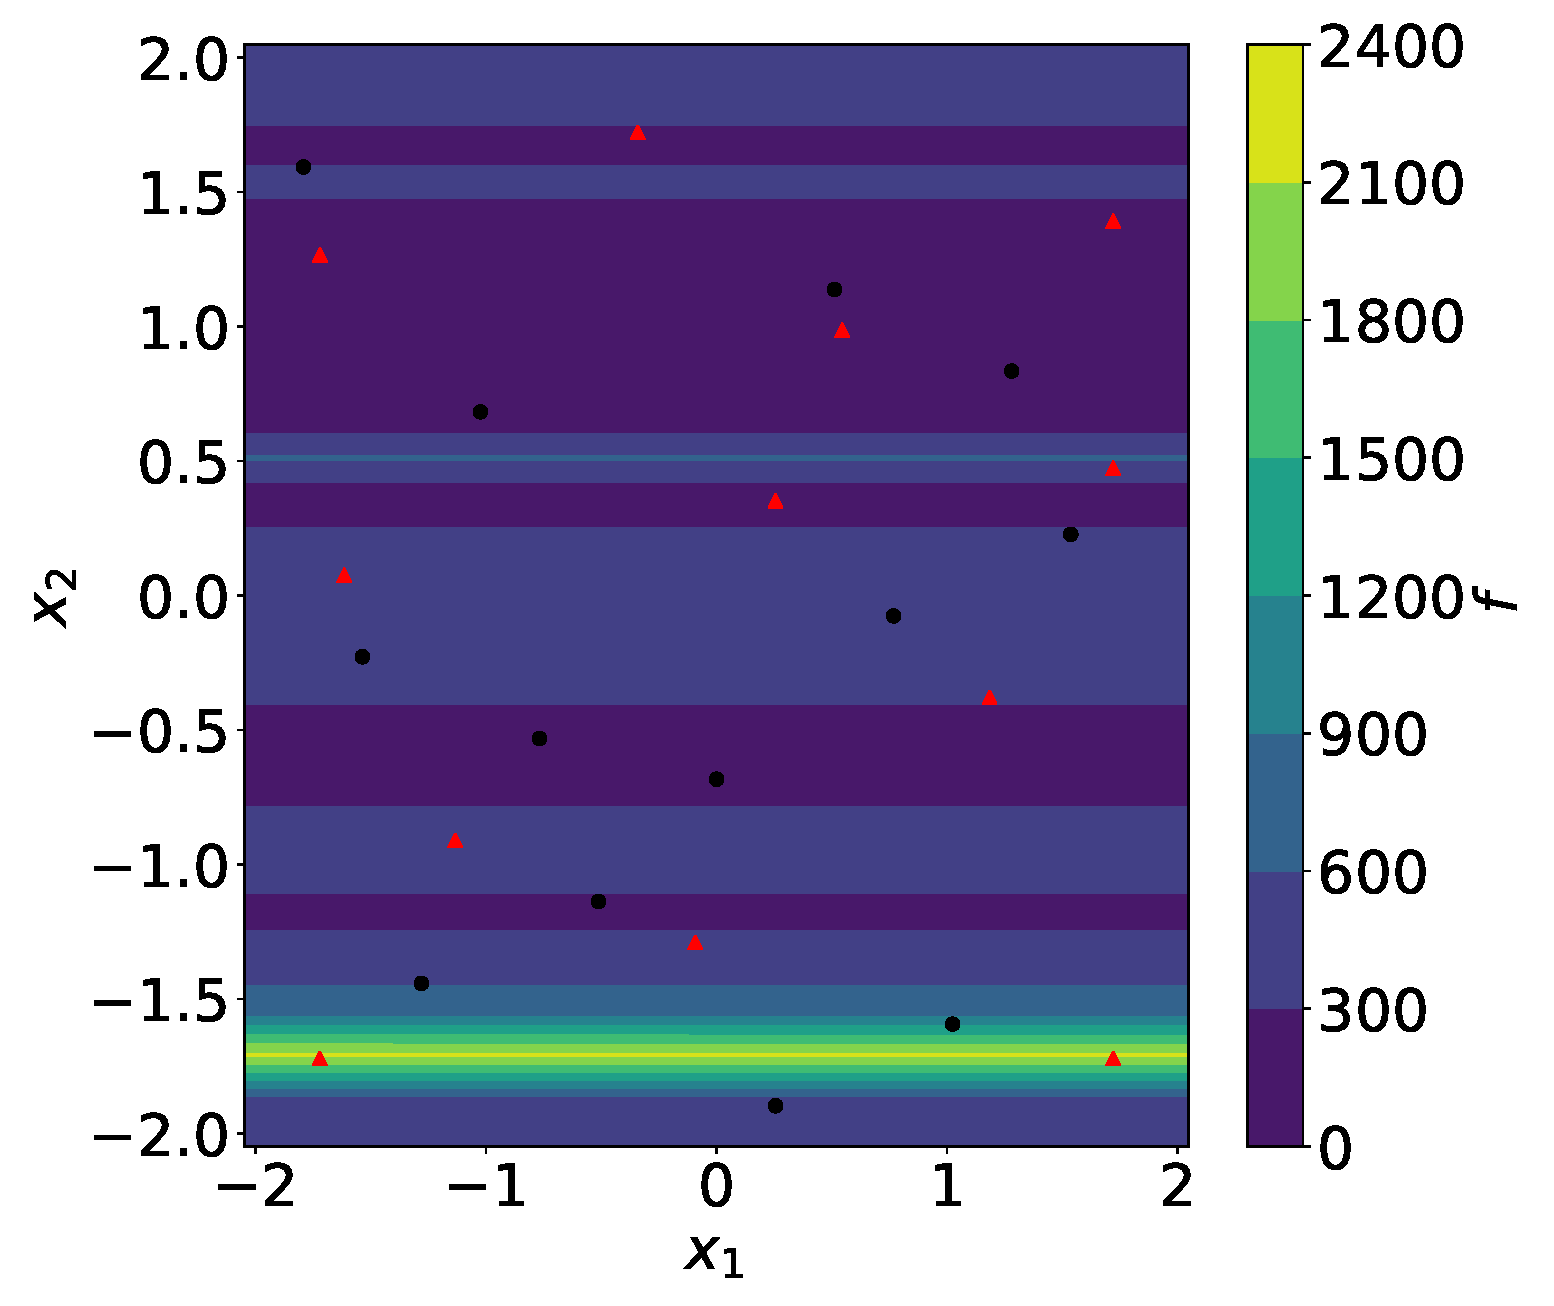
\includegraphics[width=0.47\linewidth,height=\textheight,keepaspectratio]{fig/contributions/resample/9a_2column_color-online-only_response_rosen_Ns13_sigma.pdf}}
 ~       
\subfloat[RBF: $Q_2 = 0.83$]{
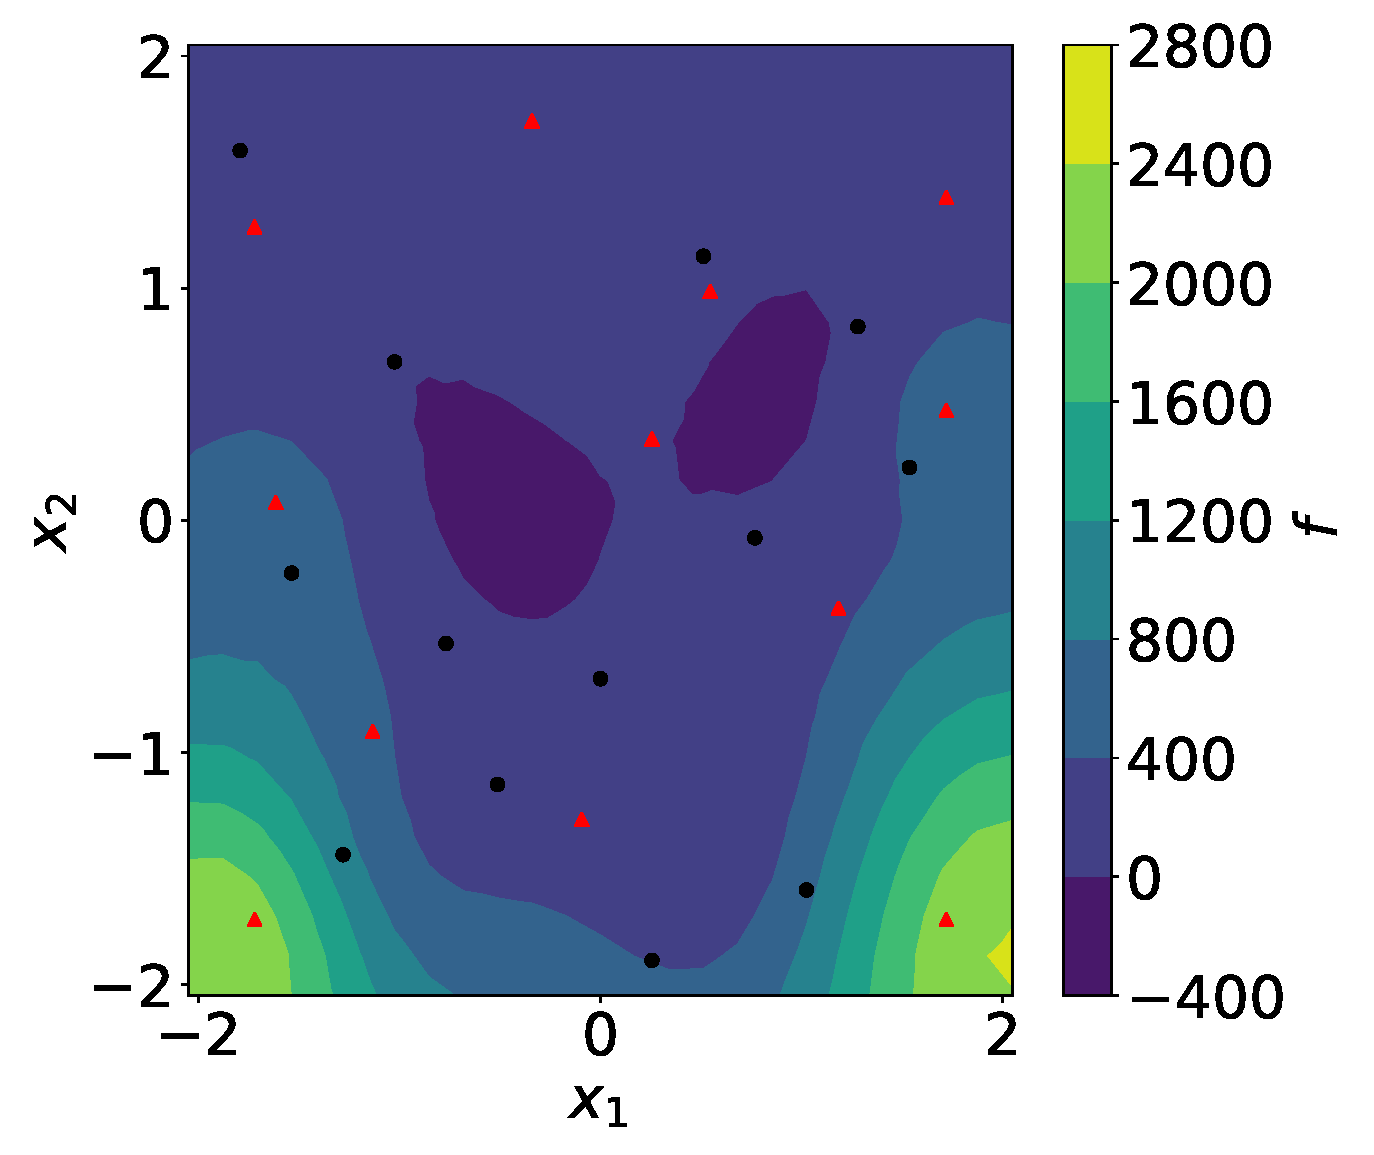
\includegraphics[width=0.47\linewidth,height=\textheight,keepaspectratio]{fig/contributions/resample/9b_2column_color-online-only_response_rosen_Ns13_sigma-RBF.pdf}}
\caption{Response surface of the \textit{Rosenbrock} function. Comparison between two models. The initial sample is composed of 13 simulations and 12 resampling points---respectively represented in dots and diamonds.}
\label{fig:methods-rosenbrock-nofit}
\end{figure*}

The other two methods share the $\sigma$ strategy, but the variability is conditioned by the LOO point. Indeed, the former only uses inference about the predictive variance whereas LOO's methods take into account the observed quality of the model.
LOO-\textit{Sobol'} is even more stable especially when the contribution of the parameters to the QoI is not even. The quality evolves quasi-linearly with the initial sample size. This is due to the initial guess on the indices. The closer the indices are converged, the better the sizing of the hypercube used by the $\sigma$ strategy. Indeed, some dimension of the hypercube could be neglected due to the indices. In the \textit{Rosenbrock} case the method behaves like LOO-$\sigma$, the importance factors are close enough so that this collapse of dimension does not occur. On the other hand, with the \textit{g-function} 4-D and \textit{g-function (i)} 11-D, the total order \textit{Sobol'} indices of the last input parameters are so small that the algorithm tends not to take into account these dimensions. Finally, for the \textit{g-function (ii)} 11-D case, more input parameters are active---meaning that their total order \textit{Sobol'} indices are greater than 0.1---, so that the improvement is not as important as with the \textit{g-function (i)} 11-D case. Still, better results are found compared to the $\sigma$ strategy. These results are comparable to the \textit{Rosenbrock} case where LOO-\textit{Sobol'} perform similarly to LOO-$\sigma$. Indeed, as the number of active parameters grows, improving the $Q_2$ would imply a better coverage of the parameter space. Thus, as the number of active dimension increases, it is expected that the optimal $Q_2$, for a given number of samples, would converge to the $Q_2$ given by the use of a low discrepancy sampling. At worst the low discrepancy sampling's $Q_2$ will be a lower bound for these methods. In realistic engineering applications, the importance of the relative contributions of the input parameters being most of the time unknown, these methods seem promising.
For each function, as the initial sample gets close to the budget, the expected improvement is reduced. This is clear with the \textit{Ishigami} function. When the initial sample is too small, the model is so poor that the points are not added efficiently. On the contrary, if we add an insufficient number of points, the impact is close to none but still there is an improvement. From the other cases, the effect of the ratio of the initial learning sample size over the total budget is not so clear. In 2-D the impact is null and after that, a ratio $>0.5$ seems appropriate.

Thus, setting aside the possible non-fitting of the data, improving the quality of the surrogate model by resampling the parameter space appears to be guaranteed in high dimensional cases and using no more than half of the budget.


\section{Conclusion}

Two new methods have been introduced in this work for resampling the parameter space in order to improve the predictivity coefficient of a surrogate model: namely LOO-$\sigma$ and LOO-\textit{Sobol'} methods. These methods do not only take advantage of the capability of Gaussian Process models to infer a prediction variance, but they use information about the observed quality of the model. It was shown that an improvement of the quality of the model is guaranteed in high dimensional cases. Compared to a resampling method based on the predicted variance only, the proposed methods behaviour appears to be more stable and reliable. We also found that the ratio of the initial learning sample space over the total budget of function evaluation should remain greater than $\numprint{0.5}$. Which is to say that no more than half of the budget should be allocated to resampling the parameter space. In any case, the initial quality of the model should be reasonable when considering these techniques.

By taking into account the physics in this process, the proposed methods will help build better models at lower costs. This will also allow Uncertainty Quantification of high-dimensional or expensive cases to be within reach.

\chapter{Uncertainty Visualization}



\section{Uncertainty Visualization of Functional Output Data}
\label{sec:uqvisu}
%In the following, the focus is put on the dimensionality of the response variable. The dimensionality of the parameter space is not taken into account as it will be treated in~\cref{sec:input}. When dealing with functional response variable, we are interested in finding the median outcome as well as to have some sort of measure of how the data spreads. 

\subsection{Dynamic Visualization of Functional Outputs' Statistics}
\label{subsec:fhop}

%A good visualization system should be expressive and effective which is to say be able:
%
%\begin{itemize}
%\item To lead a natural and accurate interpretation,
%\item Not to interfere with the data values reading.
%\end{itemize}

%Area, gradient and opacity are less effective channels as opposed to position (scatter plot) or .

%Hypothetical Outcome Plots (HOPs)~\citep{Hullman2015} is a dynamic visualization technique which consists in presenting hypothetical outcomes, sampled from the data distribution. From each outcome a plot is made and the result is presented as an animation or as several static plots. Compared to traditional static representations such as error bars, violin plots or boxplot, they showed that people make better judgment about plot containing two or three response variables.

The HOPs dynamic visualization can be applied to functional outputs~\citep{Kale2018} as in~\cref{fig:f-hops} animating successive realizations of the data (for the El Ni\~no dataset), it is noted f-HOPs. When combined to HDR criteria, each realization is discriminated taking into account the functional characteristics of the output and outliers are easily detected. This solution is complementary to the classical PDF plot for functional outputs shown in~\cref{fig:pdf} that displays the probability of monthly sea surface temperature. The median and standard deviation curves are shown but these statistics are computed point by point independently and the outliers cannot be represented. Yet, f-HOPs does not allow to exhibit multiple modes statistics that are shown by the PDF at a given location. For instance, \Cref{fig:pdf_MASCARET} shows both the functional PDF and a PDF at a precise location of the Hydrodynamics dataset. It can be noted that there are multiple modes.

%This method is to be compared with the common way of looking at such data, by mean of a PDF. \Cref{fig:pdf} shows a common static functional PDF from the same dataset. The information that can be extracted from this last figure is not as complete as the f-HOPs method in the sense that spatial correlation is not present. Indeed, the outliers as the one shown in~\cref{fig:f-hops}(b) cannot be seen in the PDF. All moments are computed without taking into account the spatial and temporal correlation. But they are computed per element of the functional output vector. In this case, the PDF does not provide additional information as it only exhibit one mode. But if looking at a more complex case as Hydrodynamics---see~\cref{sec:dataset} and ~\cref{fig:pdf_MASCARET}(a)---, the PDF plot contains a multi-modale structure---as seen in~\cref{fig:pdf_MASCARET}(b)---that is shadowed by an HDR visualization. Thus both technique are complementary.

\begin{figure*}[!h]               
\centering
\subfloat[Frame \#$n$]{
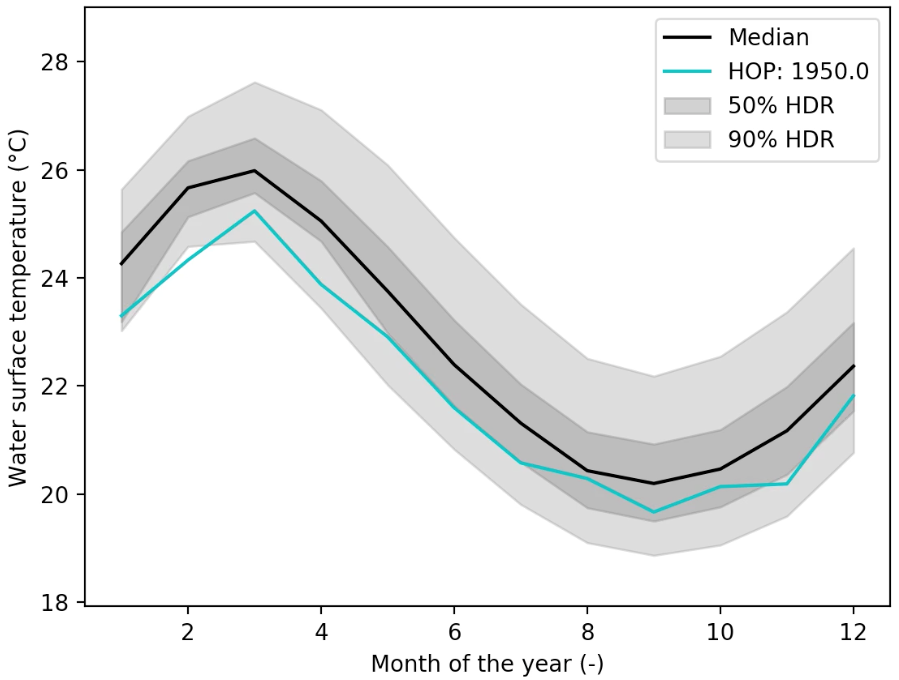
\includegraphics[width=0.45\linewidth,height=\textheight,keepaspectratio]{fig/contributions/visu/f-hops_nominal.png}}
\subfloat[Frame \#$n+1$]{
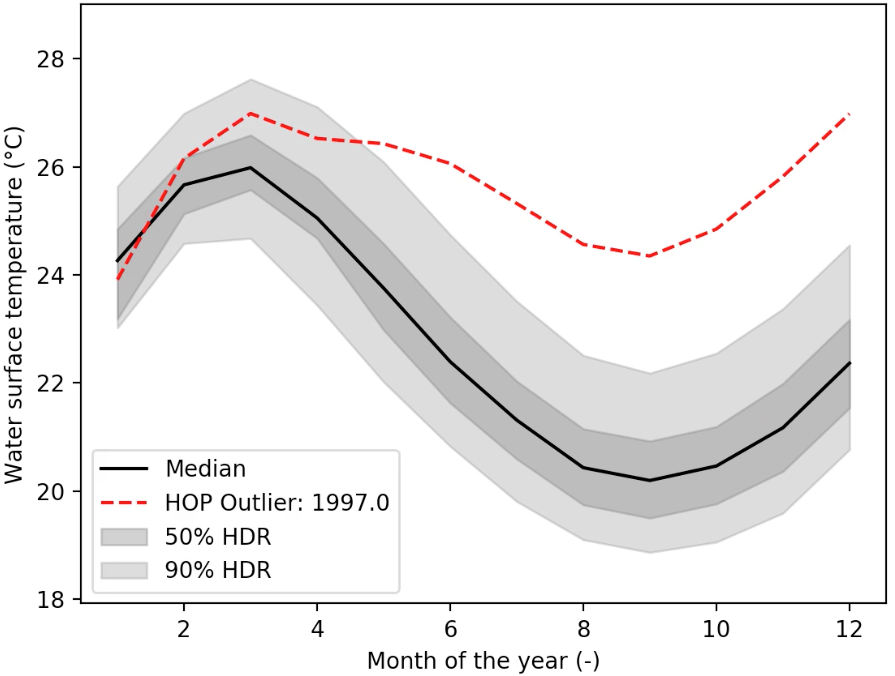
\includegraphics[width=0.45\linewidth,height=\textheight,keepaspectratio]{fig/contributions/visu/f-hops_outlier.png}} 
\caption{Functional-HOPs. \textbf{a} close to median realization. \textbf{b} outlier realization. An animated version of this figure is available as supplementary material (\hyperref[S1]{S1}).}
\label{fig:f-hops}
\end{figure*}

\begin{figure}[!h]
\centering
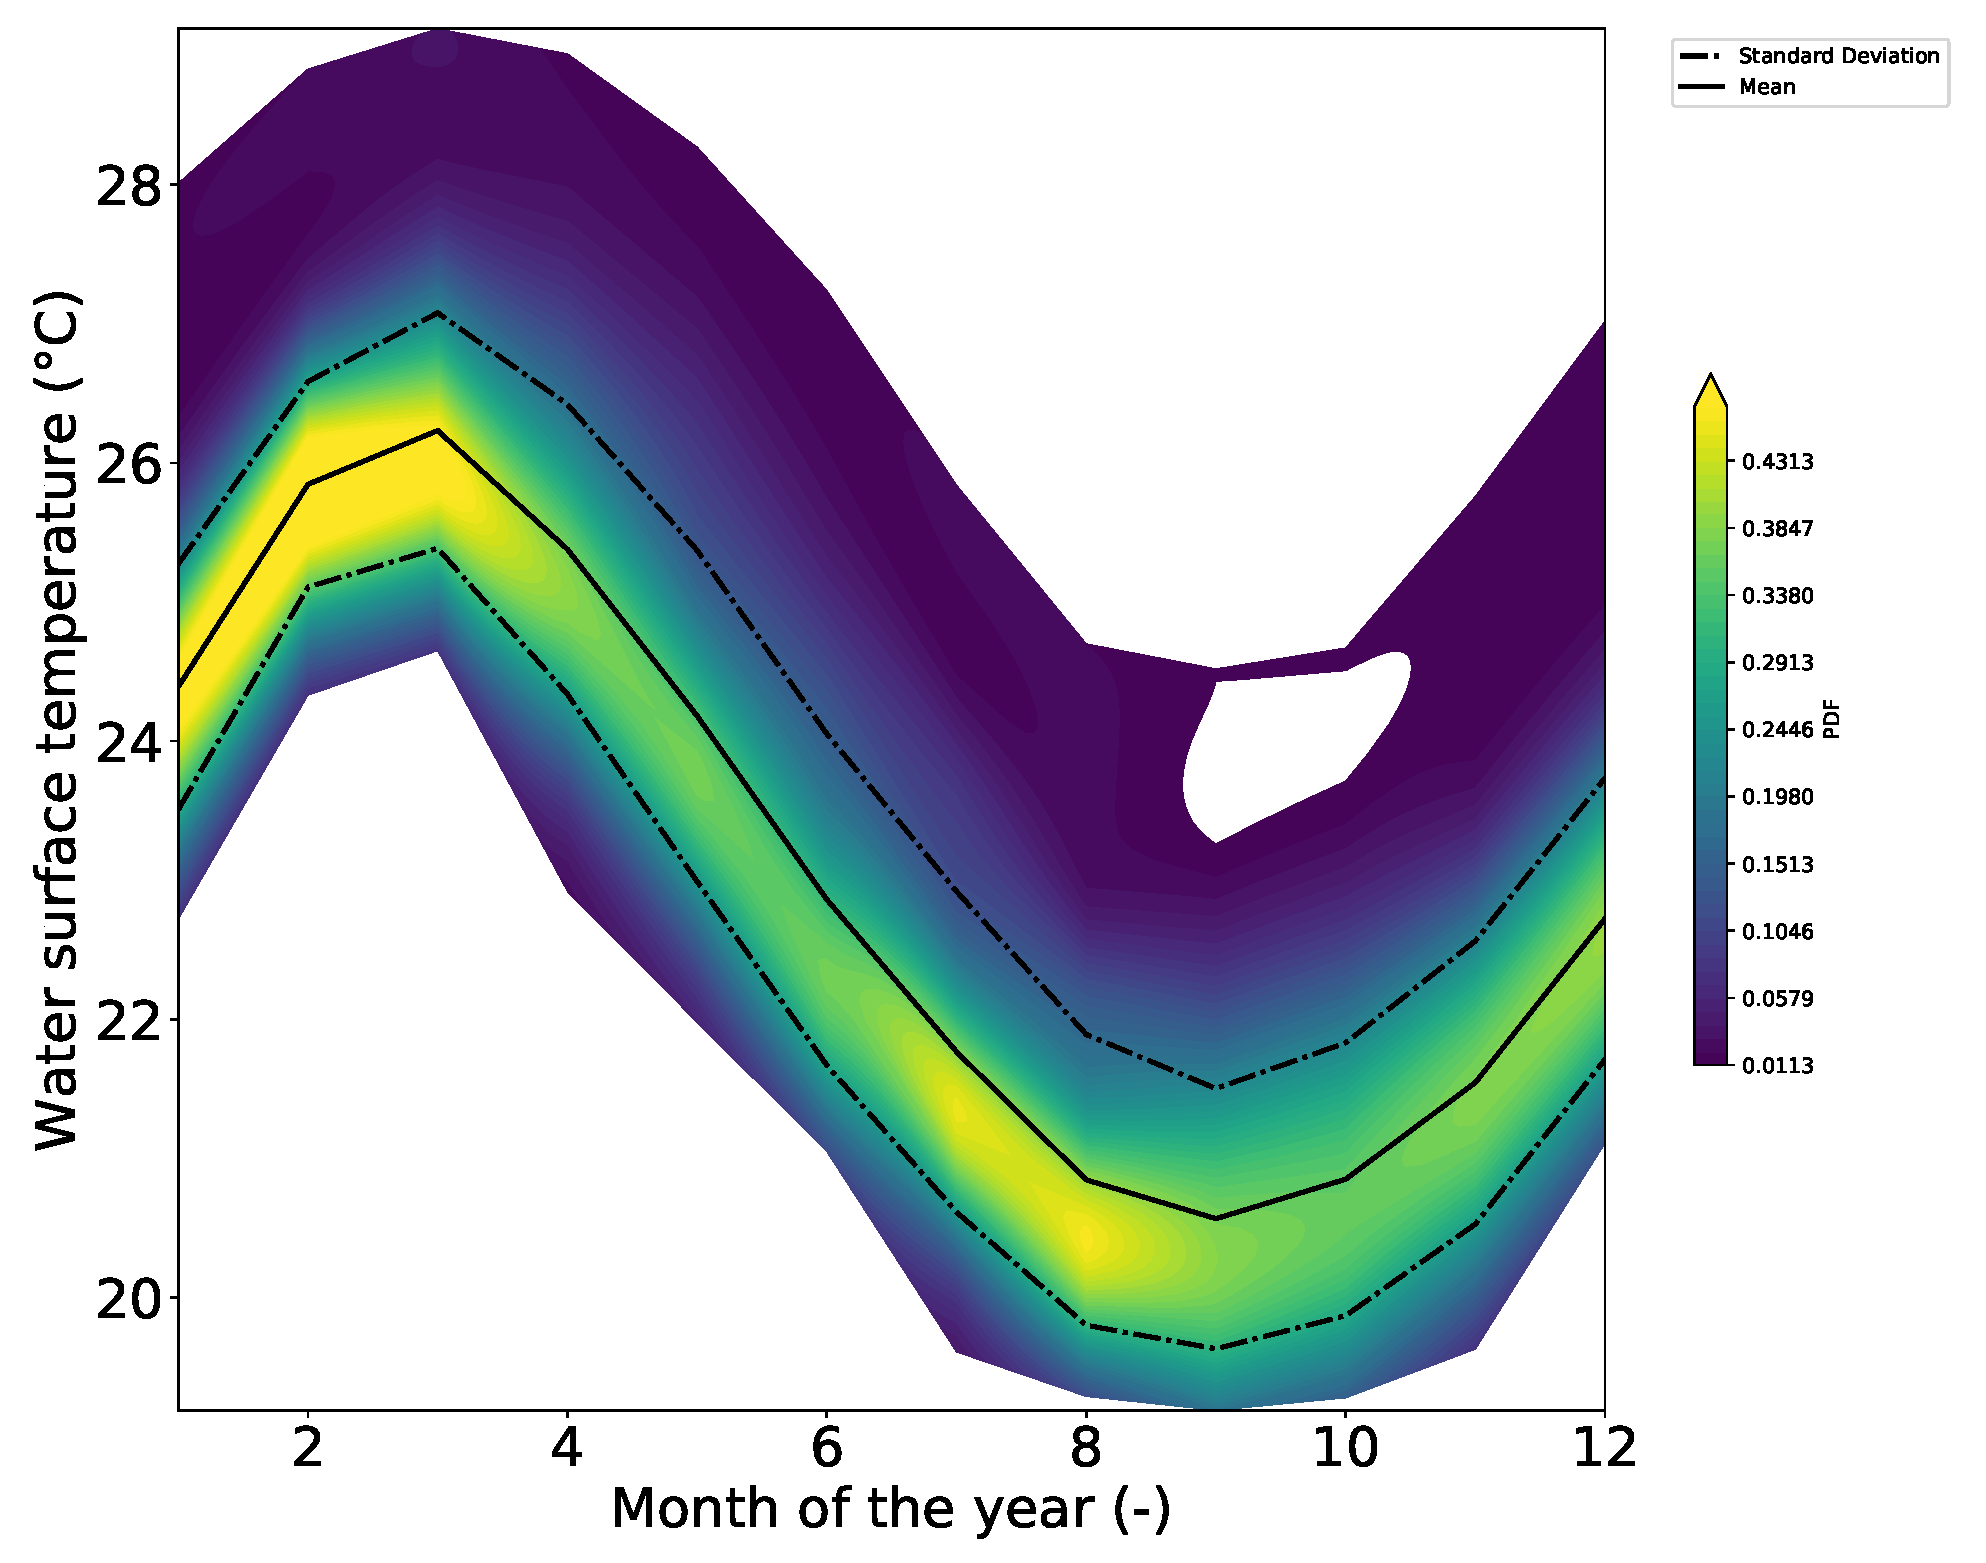
\includegraphics[width=0.8\linewidth,keepaspectratio]{fig/contributions/visu/pdf.pdf}
\caption{Functional PDF of monthly sea surface temperature. Moments are computed with respect to the 58 realizations per month of the year.}
\label{fig:pdf}
\end{figure}

\begin{figure*}[!h]               
\centering
\subfloat[]{
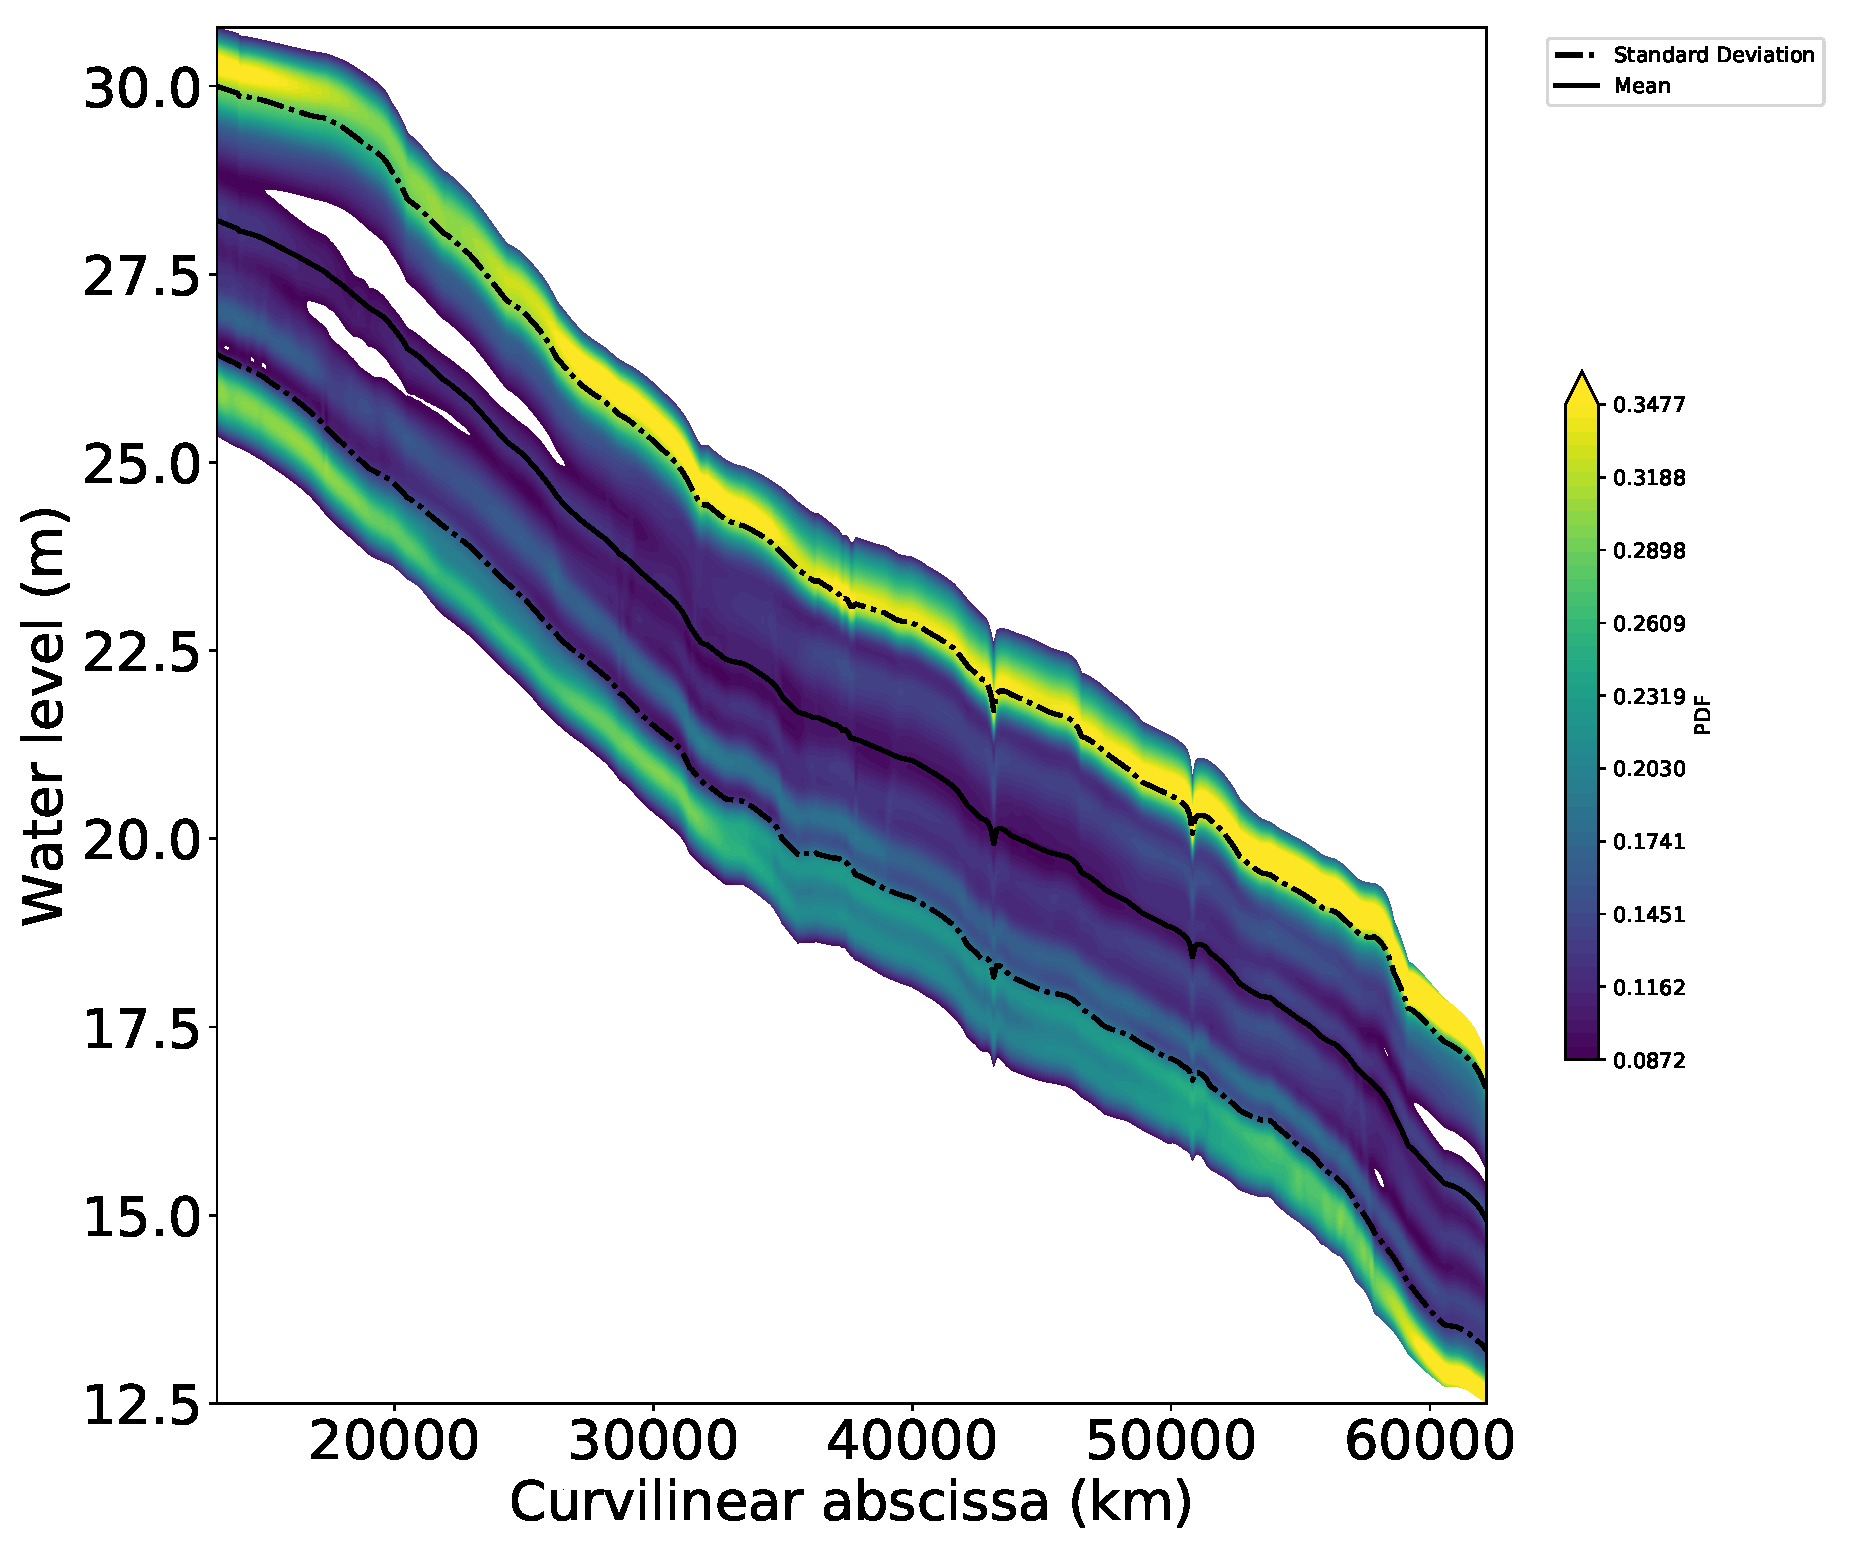
\includegraphics[width=0.45\linewidth,height=\textheight,keepaspectratio]{fig/contributions/visu/mascaret_pdf.pdf}}
\subfloat[]{
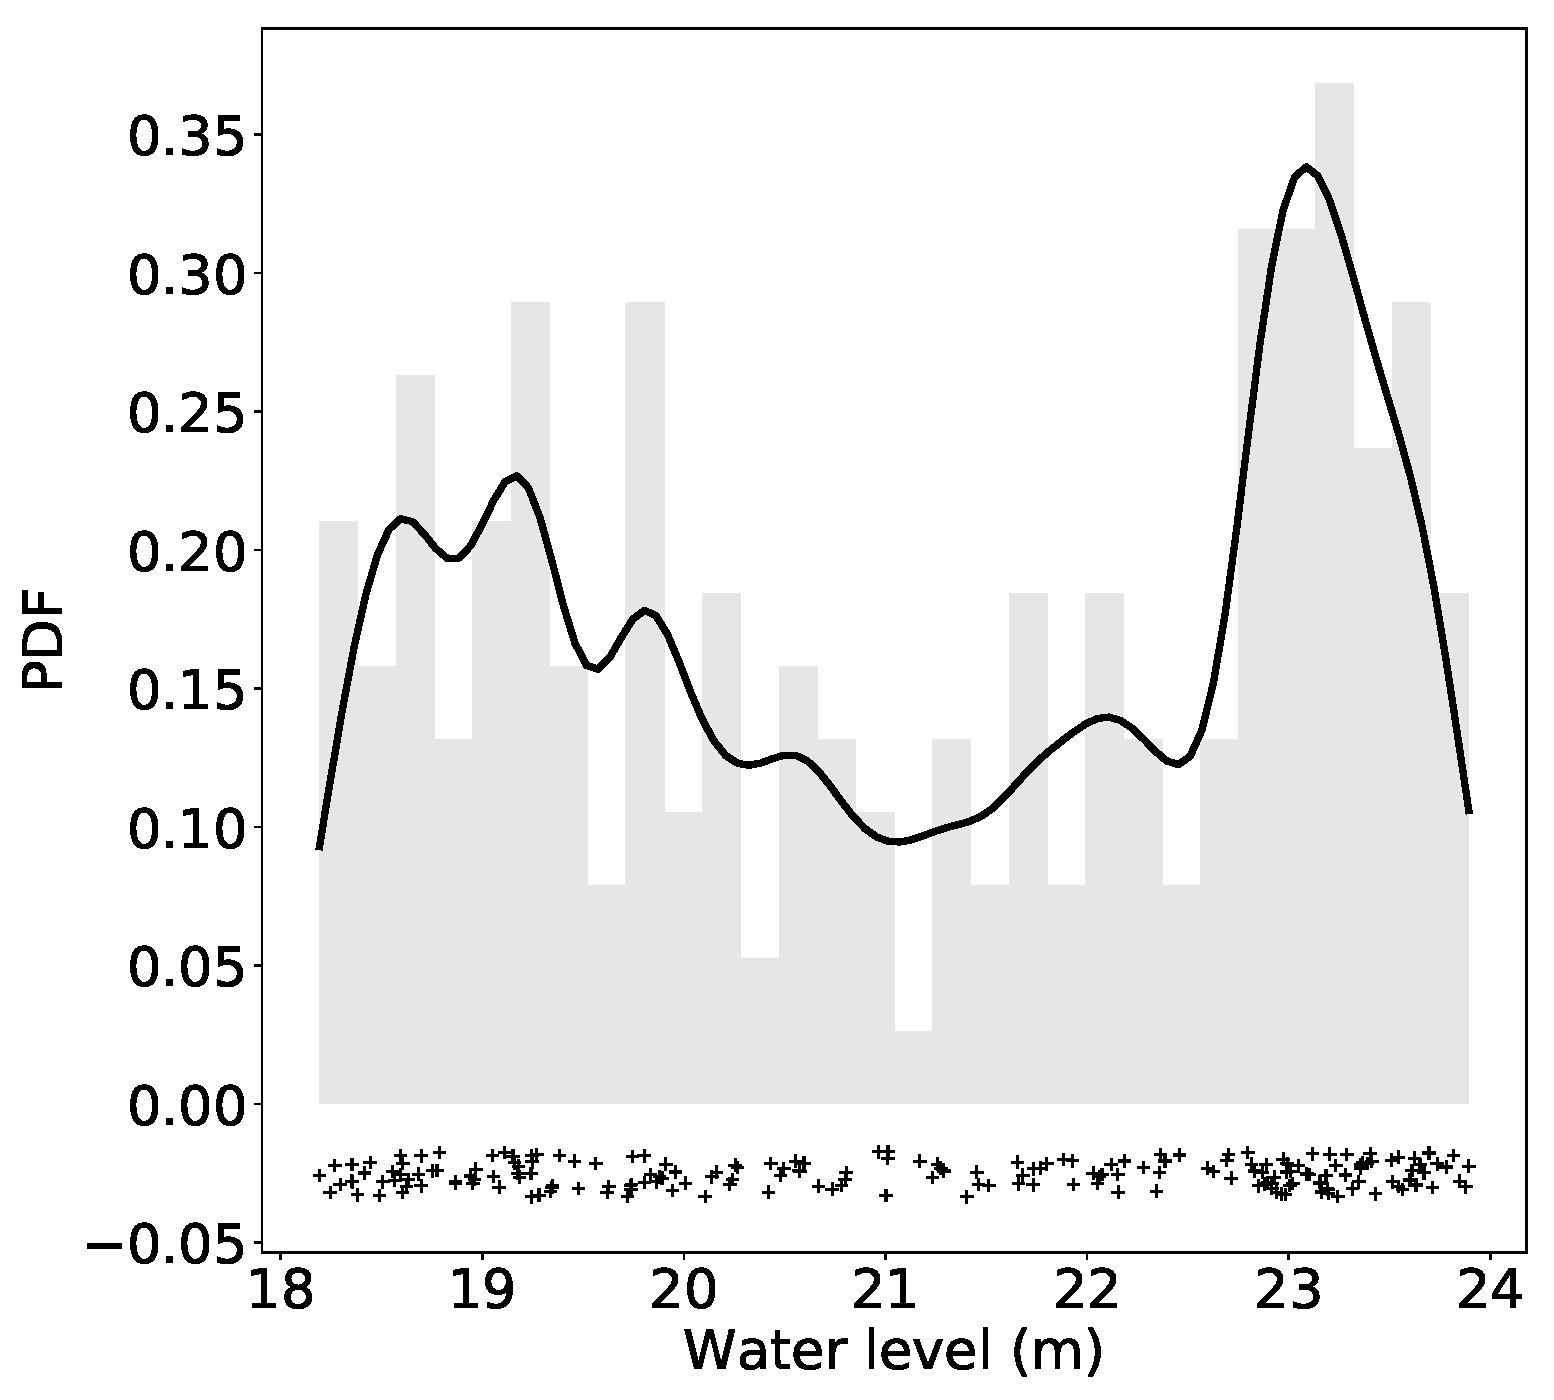
\includegraphics[width=0.45\linewidth,height=\textheight,keepaspectratio]{fig/contributions/visu/mascaret_pdf_marmande.pdf}} 
\caption{Functional PDF of the water elevation, \textbf{a} along the 463 nodes along the river reach; \textbf{b} at Marmande station (36~km) revealing a bimodal PDF.}
\label{fig:pdf_MASCARET}
\end{figure*}

\subsection{Sonification of Functional Outputs' Statistics}
\label{subsec:sound}

When the number of realizations in the dataset is limited, a static or an animated visualization, using f-HOPs and HDR metrics, allow to depict the most significant characteristics of the ensemble members. When this number increases, the animation time increases and the analysis becomes harder. Sonification comes as an alternative for meaningful analysis of the dataset: it conveniently allows to draw the attention on specific realization discriminated by the HDR metric. We propose to compute the $L_2$-norm between each realization and a reference realization within the reduced modal space.  The reference realization is here chosen as the median and is mapped into a base sound. The frequency associated with each realization increases, and the sound becomes higher as the distance between each realization and the reference increases. Evidently, the reference can differ from the median. 
\citep{Alexander2014} presents that sonification allows for well-informed understanding of a large dataset and that practitioners usually develop a physics-dependent vocabulary that is adapted to specific need as in~\citep{Hughes2003} where sound is used to discriminate the types of gravitational waves. In this context, sonification serves data exploration. It  can also be an alert system: f-HOPs augmented with HDR metric sonification allows to get a fairly monotonous sound for realizations that are close to the median, while outliers are clearly spotted as proposed in~\hyperref[S1]{S1} for the El Ni\~no dataset.

\section{Uncertainty Visualization of Large Number of Input Variables}
\label{sec:input}

\begin{figure}[!h]
\centering
\includegraphics[width=0.8\linewidth,keepaspectratio]{fig/contributions/visu/mascaret_2D.pdf}
\caption{Kiviat plot on the Hydrodynamics dataset: 2-dimensional Kiviat plane represents one sample of the data set. Colour maps the water level response variable value at Marmande (one location and one time).}
\label{fig:Kiviat_color}
\end{figure}

In the previous section, the focus was made on visualizing the response variable, not taking into account the relation between inputs and outputs. As visualizing the input alone, especially in case of small input dimension, is classical, the dual representation of input and output data remains challenging especially for large dimension functional outputs. The response surface plot is adapted when the input space is 2D or 3D. When the input space dimensions further increases, other solutions should be preferred such as parallel coordinates plot~\cite{Inselberg1985,Inselberg2009} or 3D-\emph{Kiviat} proposed by~\citep{Hackstadt1994}. In the literature, \emph{Kiviat} plot were used to map uncertainties with density criteria~\citep{VanSomeren2016} and confidence intervals are represented on a 2D plot.

In this paper, we propose to adapt the 3D-\emph{Kiviat} plot to the visualization of both input and response variable spaces. Each plane of the Kiviat represents a realization within the dataset with as many directions as the input dimensions as shown in~\cref{fig:Kiviat_color} for the hydrodynamics dataset. The input variables here correspond to the friction coefficients ($Ks1$, $Ks2$, $Ks3$) and the constant inflow $Q$; the output variable is the water level at Marmande, it is colour-coded onto the Kiviat plane. For the 3D-Kiviat, planes are stacked into a 3D object with respect to the response variable (scalar or functional) related value that is colour-coded. It should be noted that each plane is filled with only one colour to preserve readability. The benefit of 3D-Kiviat stands in the choice of both the stacking and the colouring strategies as shown in~\cref{fig:Kiviat_order} for the hydrodynamics dataset. Additionally, the 3D-Kiviat can be augmented with sound---as described in~\cref{subsec:sound}.

When representing functional output data, different stacking and colouring strategies allow to highlight different information in the dataset. Four choices of stacking and colouring are illustrated in~\cref{fig:Kiviat_order}; the stacking and colouring choices are indicated in the legend, they are achieved with respect to the response variable at a given location and time, with respect to the HDR metric or with respect to one of the input variables. In~\cref{fig:Kiviat_order}(a), stacking is done with respect to the response variable at a given location and time while the colouring is done with respect to the difference to the median realization computed with the HDR metric. This allows to get a sense of the spatial PDF represented in~\cref{fig:pdf_MASCARET} augmented with the input parameter mapping. Another possibility in~\cref{fig:Kiviat_order}(b) consists in stacking with respect to the HDR metric and colouring with respect to the response variable value. In~\cref{fig:Kiviat_order}(c), stacking is done with respect to one of the input variable (in the present case $Q$) and the colouring is done with respect to the HDR metrics. Finally, \cref{fig:Kiviat_order}(d) displays both stacking and colouring with respect to the response variable value. It should be noted that an animated version of~\cref{fig:Kiviat_order}(a) is provided in supplementary material~\cref{S2} with sounding for the HDR metric that represents the distance to the median realization and allows for a convenient analysis of the data set especially when its dimension increases.

From~\cref{fig:Kiviat_order}(a, c, d), the impact of $Q$ on the water level is easily readable; water level increases with $Q$. High water level values are also obtained for low $Ks3$ values while other parameters seem to have no significant impact on the response variable. $Ks1$ and $Ks2$ have barely any impact on the response variable. The manipulation of the animated 3D-Kiviat (\cref{S2}) is even more adapted to data analysis. The coloured HDR in~\cref{fig:Kiviat_order}(a, c) indicates how each realization differs from the median realization. It appears that stacking for colouring with respect to response variable or HDR serves different purposes. Ordering by response variable allows to discriminate which input lead to specific response variable value while ordering by HDR illustrated the dispersion of the dataset with respect to a reference realization. Sounding is a supplementary way to emphasis the information, especially for large datasets.
%To introduce its use, the Hydrodynamics dataset is used---see~\cref{sec:dataset}. Considering a sample $\mathbf{x}_{*}$ of the parameter space in $\mathcal{R}^4$, \cref{fig:Kiviat_color} shows its representation as a Kiviat plot. Nodes of the surface are positioned at values of the sample, while color maps a particular value of the model at the sample. \Cref{fig:Kiviat_order} shows 200 samples as a stack of 200 individual 2-dimensional Kiviat plot. Different stacking strategies are explored. 

%When representing functional data, the information can be conveyed by both sound and coloring sound or using particular stacking and coloring strategies. For instance, stacking can be colored by their difference to the median realization computed by HDR. Indeed, to preserve usability, the surface can only be filled using one color. Using this stacking scheme could add this functional information. }


%Thus, each sample is treated as a 2-dimensional planar Kiviat plot, with as many direction as the number of inputs. The surface is uniformly colored to transmit extra information. \Cref{fig:Kiviat_color} presents the extension of the 2-dimensional Kiviat plot colored by the response variable. Finally, all Kiviats from the samples are stacked together forming a 3-dimensional object.}

%Visualizing the input parameter space itself is classically done by looking at 2-dimensional subprojections which is not specially challenging. But, if we are interested in both the response variable and the sample, this can be challenging. And the problem is even worse when considering functional response variable.

%In this case, there are 5 axis (one per parameter and one for the response variable) and each line corresponds to a realization. By filtering out the response variable, one can arrive to the same conclusion that highest values of the response variable are conditioned by lowest values of $Ks3$, no matter the values of $Ks1$ and $Ks2$. However, the monotonous relationship found on $Q$ is difficult to grasp as well as the structure on $Ks3$. Thus, both methods are able to observe some clustering but particular behaviours---as the monotonous relationship on $Q$---are harder if not impossible to get.

\begin{figure*}[!h]               
\centering
\subfloat[Stacking: response variable - Colouring: HDR]{
\includegraphics[width=0.47\linewidth,height=\textheight,keepaspectratio]{fig/contributions/visu/mascaret_kiviat_qoi_hdr.pdf}}
 ~       
\subfloat[Stacking: HDR - Colouring: response variable]{
\includegraphics[width=0.47\linewidth,height=\textheight,keepaspectratio]{fig/contributions/visu/mascaret_kiviat_hdr_qoi.pdf}}

\subfloat[Stacking: $Q$ - Colouring: HDR]{
\includegraphics[width=0.47\linewidth,height=\textheight,keepaspectratio]{fig/contributions/visu/mascaret_kiviat_q_hdr.pdf}}
~
\subfloat[Stacking: response variable - Colouring: response variable]{
\includegraphics[width=0.42\linewidth,height=\textheight,keepaspectratio]{fig/contributions/visu/mascaret_kiviat_qoi_qoi.pdf}}
\caption{Kiviat plot on the Hydrodynamics dataset: comparison of different stacking orders and colour map strategies. \textbf{a} samples stacked by response variable and coloured by HDR. \textbf{b} samples stacked by HDR and coloured by response variable. \textbf{c} samples stacked by $Q$ and coloured by HDR. \textbf{d samples} stacked by response variable and coloured by response variable. An animated version of \textbf{a} is available (\hyperref[S2]{S2}).}
\label{fig:Kiviat_order}
\end{figure*}

3D-Kiviat comes as a complementary tool to classical sensitivity analysis criteria such as \emph{Sobol'} indices~\citep{Saltelli2007}. When computed on a large dataset (100 000 members) for the hydrodynamics example and averaged over space, these indices show that most of the variance of the water level is explained by $Q$ with $S_Q=0.98$. A small part of the variance is explained by $Ks3$ as $S_{Ks3} = 0.14$ and even smaller by $Ks1$ and $Ks2$ with $S_{Ks1}=0.01$ and $S_{Ks2} = 0.07$.

While the \emph{Sobol'} indices quantify the importance of each parameter on the response variable's variance, they do not indicate the nature of these contributions. Indeed, it is stated that $Q$ has a significant impact but from~\cref{fig:Kiviat_order}(a, c, d), we can also add that the contribution is monotonous. Additionally, the weak impact of $Ks1$ and $Ks2$ is confirmed by the lack of a pattern in the 3D-Kiviat along these axes. Finally, while the $Ks3$ Sobol index is weak, the 3D-Kiviat indicates that small $Ks3$ values lead to high-water level values.

It appears that 3D-Kiviat plot becomes difficult to manipulate when the dimension of the input parameter increases ($>10$). To overcome this caveat, we have designed a method to generate a surface mesh of the Kiviat plot as shown in~\cref{fig:mesh}. This allows the use of regular CAD viewers and thus facilitates the manipulation of the 3D object as well as the comprehension of the data structure. The construction is based on a vertex-vertex representation using quadrilateral elements. An animated version of~\cref{fig:mesh} is provided in~\cref{S3} with stacking with respect to the response variable value, colouring with respect to the HDR metric, then colouring with respect to the input parameters in~\cref{S4}. 

%\pamphile{OK on peut enlever si tu veux}
%\sophie{JE NE PENSE PAS QUE CES 2 PHRASES AIENT UN INTERET  : As it can be seen in~\cref{fig:mesh}, this technique is not only convenient but it allows different kind of post-treatment. Another thing to notice is that as the number of parameter increases, the order in which the parameters are arranged can help. Correlations between parameters are more likely to exists with parameters linked with each other.}

\begin{figure}[!h]
\centering
\includegraphics[width=0.6\linewidth,keepaspectratio]{fig/contributions/visu/mascaret_mesh_points.pdf}
\caption{3-dimensional Kiviat in point representation stacking with respect to the response variable and colouring with respect to the input parameter. An animated version of this figure is available with stacking with respect to the response variable and colouring with respect to the HDR metric in~\hyperref[S3]{S3} and with respect to the input parameter in ~\hyperref[S4]{S4}.}
\label{fig:mesh}
\end{figure}

The analysis from 3D-Kiviat is similar to that drawn from the parallel coordinates plot in~\Cref{fig:cobweb-Kiviat}. The latter consists of $n+1$ parallel axes, with $n=4$ the number of input parameters for the hydrodynamics dataset. The last axis is dedicated to the output value, here water level at Marmande. Each grey line corresponds to one realization in the dataset; the red lines are discriminated for high-water level values resulting from high $Q$ and small $Ks3$, independently of $Ks1$ and $Ks2$. It should be noted that parallel coordinate plot is not adapted to simultaneous representation of response variable and HDR metrics contrary to 3D-Kiviat. Finally, the linear relationship between water level and $Q$ that was clear on the 3D-Kiviat in not readable on the parallel coordinate plot that is more adapted to clustering with the possibility of advanced strategies proposed by~\citep{Claessen2011,Raidou2016}.

\begin{figure}[!h]
\centering
\includegraphics[width=0.8\linewidth,keepaspectratio]{fig/contributions/visu/mascaret_cobweb.pdf}
\caption{Parallel coordinates plot for the hydrodynamics dataset with 80\% of the lowest values of response variable filtered out (in grey) and high values in red.}
\label{fig:cobweb-Kiviat}
\end{figure}

The specific case of a 2D input space is treated with a \emph{Tree plot} solution where Kiviat coloured planes are replaced by coloured segments that are stacked and coloured regarding to response variable related value. The vertical stacking and colouring are achieved with respect to the response variable value. The HDR metric is encoded as an azimutal component: the angle is null if the realization corresponds to the median and the angle increases as the realization differs to the median. \Cref{fig:tree} displays a tree plot for the hydrodynamics dataset where $Ks1$ and $Ks2$ are not accounted for (since they were previously shown to have barely any impact on the response variable) and the response variable is the water level at Marmande. Here again, stacking, colouring, angle and eventually sounding strategies can be adapted to convey information on a dataset and efficiently enhance meaningful information.

%** To overcome this issue, we derived from the 3-dimensional Kiviat plot to only show a succession of segments instead of plane. Appart from showing only existing dimensions, the third dimension is used to encode the functional information of the response variable otherwise encoded with sound. This information is encoded as an azimutal component. This visualization method is hereafter referred to as the Tree plot. \Cref{fig:tree} shows the same data as~\cref{fig:Kiviat_order} but here only $Ks3$ and $Q$ are considered. $Q$ can still be seen as the most impacting parameter on the response variable but this visualization allows to also perceive at the same time the functional information of the case. 
%By playing with the stacking order, the coloring scheme and selecting only a subset of parameters, one can introduce repetition to encode the same information. This can help to convey a particular information and even help people with disabilities.
%Hence, for 2-dimensional cases, it allows to return to a static visualization technique.
%This technique can also be applied to lower dimensional cases. But 3-dimensions being required to create a surface, dummy dimensions set to constant values are added to have at least 3-dimensions. This approach works but can be misleading as it shows dimensions that does not exists.

\begin{figure}[!h]
\centering
\includegraphics[width=0.6\linewidth,keepaspectratio]{fig/contributions/visu/mascaret_tree.pdf}
\caption{Tree plot for the hydrodynamics dataset considering the most significant parameters $Ks3$ and $Q$. Here the response variable (water level at Marmande) is represented by stacked and coloured segments and HDR metric is represented by the azimutal component.}
\label{fig:tree}
\end{figure}




